\documentclass[]{report}
\usepackage{lmodern}
\usepackage{amssymb,amsmath}
\usepackage{ifxetex,ifluatex}
\usepackage{fixltx2e} % provides \textsubscript
\ifnum 0\ifxetex 1\fi\ifluatex 1\fi=0 % if pdftex
  \usepackage[T1]{fontenc}
  \usepackage[utf8]{inputenc}
\else % if luatex or xelatex
  \ifxetex
    \usepackage{mathspec}
  \else
    \usepackage{fontspec}
  \fi
  \defaultfontfeatures{Ligatures=TeX,Scale=MatchLowercase}
\fi
% use upquote if available, for straight quotes in verbatim environments
\IfFileExists{upquote.sty}{\usepackage{upquote}}{}
% use microtype if available
\IfFileExists{microtype.sty}{%
\usepackage{microtype}
\UseMicrotypeSet[protrusion]{basicmath} % disable protrusion for tt fonts
}{}
\usepackage[margin=1in]{geometry}
\usepackage{hyperref}
\hypersetup{unicode=true,
            pdftitle={Homework Part 2},
            pdfauthor={Vinicio Haro; Sang Yoon (Andy) Hwang; Julian McEachern; Jeremy O'Brien; Bethany Poulin},
            pdfborder={0 0 0},
            breaklinks=true}
\urlstyle{same}  % don't use monospace font for urls
\usepackage{color}
\usepackage{fancyvrb}
\newcommand{\VerbBar}{|}
\newcommand{\VERB}{\Verb[commandchars=\\\{\}]}
\DefineVerbatimEnvironment{Highlighting}{Verbatim}{commandchars=\\\{\}}
% Add ',fontsize=\small' for more characters per line
\usepackage{framed}
\definecolor{shadecolor}{RGB}{248,248,248}
\newenvironment{Shaded}{\begin{snugshade}}{\end{snugshade}}
\newcommand{\KeywordTok}[1]{\textcolor[rgb]{0.13,0.29,0.53}{\textbf{#1}}}
\newcommand{\DataTypeTok}[1]{\textcolor[rgb]{0.13,0.29,0.53}{#1}}
\newcommand{\DecValTok}[1]{\textcolor[rgb]{0.00,0.00,0.81}{#1}}
\newcommand{\BaseNTok}[1]{\textcolor[rgb]{0.00,0.00,0.81}{#1}}
\newcommand{\FloatTok}[1]{\textcolor[rgb]{0.00,0.00,0.81}{#1}}
\newcommand{\ConstantTok}[1]{\textcolor[rgb]{0.00,0.00,0.00}{#1}}
\newcommand{\CharTok}[1]{\textcolor[rgb]{0.31,0.60,0.02}{#1}}
\newcommand{\SpecialCharTok}[1]{\textcolor[rgb]{0.00,0.00,0.00}{#1}}
\newcommand{\StringTok}[1]{\textcolor[rgb]{0.31,0.60,0.02}{#1}}
\newcommand{\VerbatimStringTok}[1]{\textcolor[rgb]{0.31,0.60,0.02}{#1}}
\newcommand{\SpecialStringTok}[1]{\textcolor[rgb]{0.31,0.60,0.02}{#1}}
\newcommand{\ImportTok}[1]{#1}
\newcommand{\CommentTok}[1]{\textcolor[rgb]{0.56,0.35,0.01}{\textit{#1}}}
\newcommand{\DocumentationTok}[1]{\textcolor[rgb]{0.56,0.35,0.01}{\textbf{\textit{#1}}}}
\newcommand{\AnnotationTok}[1]{\textcolor[rgb]{0.56,0.35,0.01}{\textbf{\textit{#1}}}}
\newcommand{\CommentVarTok}[1]{\textcolor[rgb]{0.56,0.35,0.01}{\textbf{\textit{#1}}}}
\newcommand{\OtherTok}[1]{\textcolor[rgb]{0.56,0.35,0.01}{#1}}
\newcommand{\FunctionTok}[1]{\textcolor[rgb]{0.00,0.00,0.00}{#1}}
\newcommand{\VariableTok}[1]{\textcolor[rgb]{0.00,0.00,0.00}{#1}}
\newcommand{\ControlFlowTok}[1]{\textcolor[rgb]{0.13,0.29,0.53}{\textbf{#1}}}
\newcommand{\OperatorTok}[1]{\textcolor[rgb]{0.81,0.36,0.00}{\textbf{#1}}}
\newcommand{\BuiltInTok}[1]{#1}
\newcommand{\ExtensionTok}[1]{#1}
\newcommand{\PreprocessorTok}[1]{\textcolor[rgb]{0.56,0.35,0.01}{\textit{#1}}}
\newcommand{\AttributeTok}[1]{\textcolor[rgb]{0.77,0.63,0.00}{#1}}
\newcommand{\RegionMarkerTok}[1]{#1}
\newcommand{\InformationTok}[1]{\textcolor[rgb]{0.56,0.35,0.01}{\textbf{\textit{#1}}}}
\newcommand{\WarningTok}[1]{\textcolor[rgb]{0.56,0.35,0.01}{\textbf{\textit{#1}}}}
\newcommand{\AlertTok}[1]{\textcolor[rgb]{0.94,0.16,0.16}{#1}}
\newcommand{\ErrorTok}[1]{\textcolor[rgb]{0.64,0.00,0.00}{\textbf{#1}}}
\newcommand{\NormalTok}[1]{#1}
\usepackage{graphicx,grffile}
\makeatletter
\def\maxwidth{\ifdim\Gin@nat@width>\linewidth\linewidth\else\Gin@nat@width\fi}
\def\maxheight{\ifdim\Gin@nat@height>\textheight\textheight\else\Gin@nat@height\fi}
\makeatother
% Scale images if necessary, so that they will not overflow the page
% margins by default, and it is still possible to overwrite the defaults
% using explicit options in \includegraphics[width, height, ...]{}
\setkeys{Gin}{width=\maxwidth,height=\maxheight,keepaspectratio}
\IfFileExists{parskip.sty}{%
\usepackage{parskip}
}{% else
\setlength{\parindent}{0pt}
\setlength{\parskip}{6pt plus 2pt minus 1pt}
}
\setlength{\emergencystretch}{3em}  % prevent overfull lines
\providecommand{\tightlist}{%
  \setlength{\itemsep}{0pt}\setlength{\parskip}{0pt}}
\setcounter{secnumdepth}{0}

%%% Use protect on footnotes to avoid problems with footnotes in titles
\let\rmarkdownfootnote\footnote%
\def\footnote{\protect\rmarkdownfootnote}

%%% Change title format to be more compact
\usepackage{titling}

% Create subtitle command for use in maketitle
\newcommand{\subtitle}[1]{
  \posttitle{
    \begin{center}\large#1\end{center}
    }
}

\setlength{\droptitle}{-2em}

  \title{Homework Part 2}
    \pretitle{\vspace{\droptitle}\centering\huge}
  \posttitle{\par}
    \author{Vinicio Haro \\ Sang Yoon (Andy) Hwang \\ Julian McEachern \\ Jeremy O'Brien \\ Bethany Poulin}
    \preauthor{\centering\large\emph}
  \postauthor{\par}
    \date{}
    \predate{}\postdate{}
  
% set plain style for page numbers
\pagestyle{plain}
\raggedbottom

% change font
\usepackage{fontspec}
\setmainfont{Arial}

% create color block quotes
\usepackage[dvipsnames]{xcolor}
\definecolor{navyblue}{RGB}{16, 52, 166}
\definecolor{stealblue}{RGB}{72, 90, 122}
\usepackage{tcolorbox}     
\newtcolorbox{question}[1]{colback=white, colframe=navyblue ,fonttitle=\bfseries, title=#1}

\newtcolorbox{subquestion}[1]{colback=white,colframe=white, coltitle=navyblue!75!black, detach title, before upper={\tcbtitle\quad\hangindent7mm}, title={#1},fonttitle=\bfseries, fontupper=\bfseries}


\usepackage{xcolor}
\usepackage{sectsty}
\usepackage{etoolbox}
\usepackage{titling}

\usepackage{titling}
\pretitle{\begin{flushright}\Huge\color{navyblue}\textbf}
\posttitle{\par\Large\color{gray}Data 624 - Predictive Analytics\linebreak 16 December 2019\end{flushright}}
\preauthor{\begin{flushright}\large \lineskip 0.5em\textbf{Group Members:}\linebreak\textit}
\postauthor{\par\end{flushright}}
\predate{\begin{flushright}\large}
\postdate{\par\end{flushright}}




% remove "chapter" from chapter title
\usepackage{titlesec}
\titleformat{\chapter}
  {\normalfont\color{navyblue}\LARGE\bfseries}{\thechapter}{1em}{}
\titlespacing*{\chapter}{0pt}{3.5ex plus 1ex minus .2ex}{2.3ex plus .2ex}


% margins
\usepackage[margin=1in]{geometry}

% kable 
\usepackage{tabu}
\usepackage{float} 
\usepackage{booktabs}
\usepackage[font={color=navyblue,bf}]{caption}

% multicolumn
\usepackage{multicol}
\usepackage{booktabs}
\usepackage{longtable}
\usepackage{array}
\usepackage{multirow}
\usepackage{wrapfig}
\usepackage{float}
\usepackage{colortbl}
\usepackage{pdflscape}
\usepackage{tabu}
\usepackage{threeparttable}
\usepackage{threeparttablex}
\usepackage[normalem]{ulem}
\usepackage{makecell}
\usepackage{xcolor}

\begin{document}
\maketitle

{
\setcounter{tocdepth}{2}
\tableofcontents
}
\chapter*{Getting Started}\label{Overview}
\addcontentsline{toc}{chapter}{Getting Started}

\section{Dependencies}\label{dependencies}

\begin{Shaded}
\begin{Highlighting}[]
\CommentTok{# Predicitve Modeling}
\KeywordTok{libraries}\NormalTok{(}\StringTok{"AppliedPredictiveModeling"}\NormalTok{, }\StringTok{"mice"}\NormalTok{, }\StringTok{"caret"}\NormalTok{, }\StringTok{"tidyverse"}\NormalTok{, }
    \StringTok{"impute"}\NormalTok{, }\StringTok{"pls"}\NormalTok{, }\StringTok{"caTools"}\NormalTok{, }\StringTok{"mlbench"}\NormalTok{, }\StringTok{"randomForest"}\NormalTok{, }\StringTok{"party"}\NormalTok{, }
    \StringTok{"gbm"}\NormalTok{, }\StringTok{"Cubist"}\NormalTok{, }\StringTok{"rpart"}\NormalTok{)}
\CommentTok{# Formatting Libraries}
\KeywordTok{libraries}\NormalTok{(}\StringTok{"default"}\NormalTok{, }\StringTok{"knitr"}\NormalTok{, }\StringTok{"kableExtra"}\NormalTok{, }\StringTok{"gridExtra"}\NormalTok{, }\StringTok{"sqldf"}\NormalTok{, }
    \StringTok{"tibble"}\NormalTok{)}
\CommentTok{# Plotting Libraries}
\KeywordTok{libraries}\NormalTok{(}\StringTok{"ggplot2"}\NormalTok{, }\StringTok{"grid"}\NormalTok{, }\StringTok{"ggfortify"}\NormalTok{, }\StringTok{"rpart.plot"}\NormalTok{)}

\CommentTok{# Data Wrangling}
\KeywordTok{library}\NormalTok{(AppliedPredictiveModeling)}
\KeywordTok{library}\NormalTok{(mice)}
\KeywordTok{library}\NormalTok{(caret)}
\KeywordTok{library}\NormalTok{(tidyverse)}
\KeywordTok{library}\NormalTok{(pls)}
\KeywordTok{library}\NormalTok{(caTools)}
\KeywordTok{library}\NormalTok{(mlbench)}
\KeywordTok{library}\NormalTok{(stringr)}

\CommentTok{# Formatting}
\KeywordTok{library}\NormalTok{(default)}
\KeywordTok{library}\NormalTok{(knitr)}
\KeywordTok{library}\NormalTok{(kableExtra)}

\CommentTok{# Plotting}
\KeywordTok{library}\NormalTok{(ggplot2)}
\KeywordTok{library}\NormalTok{(grid)}
\KeywordTok{library}\NormalTok{(ggfortify)}
\KeywordTok{library}\NormalTok{(gridExtra)}
\end{Highlighting}
\end{Shaded}

\newpage

\chapter*{Assignment 1}\label{AS-1}
\addcontentsline{toc}{chapter}{Assignment 1}

\addcontentsline{toc}{subsection}{Kuhn and Johnson 6.3}

\begin{question}{Kuhn and Johnson 6.3}A chemical manufacturing process for a pharmaceutical product was discussed in Sect.1.4. In this problem, the objective is to understand the relationship between biological measurements of the raw materials (predictors), measurements of the manufacturing process (predictors), and the response of product yield. Biological predictors cannot be changed but can be used to assess the quality of the raw material before processing. On the other hand, manufacturing process predictors can be changed in the manufacturing process. Improving product yield by 1\% will boost revenue by approximately one hundred thousand dollars per batch:\end{question}

\begin{subquestion}{(a).}Start R and use these commands to load the data:
\end{subquestion}

\begin{Shaded}
\begin{Highlighting}[]
\KeywordTok{data}\NormalTok{(}\StringTok{"ChemicalManufacturingProcess"}\NormalTok{)}
\end{Highlighting}
\end{Shaded}

The matrix \texttt{processPredictors} contains the 57 predictors (12
describing the input biological material and 45 describing the process
predictors) for the 176 manufacturing runs. Yield contains the percent
yield for each run. Using a histogram, we examined the distribution of
\texttt{Yield} and found that the response variable appears unimodal
with a normal distribution.

\begin{center}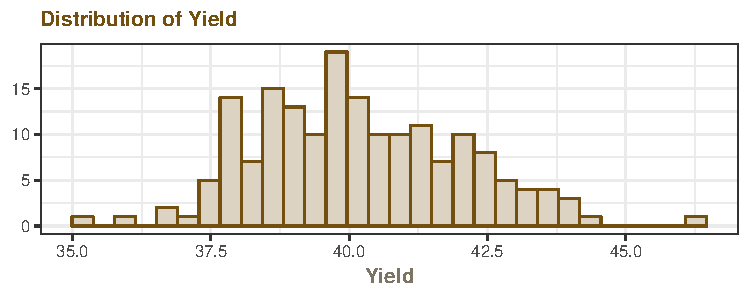
\includegraphics{Homework-Two2_files/figure-latex/kj-6.3a-plot-1} \end{center}

\begin{subquestion}{(b).} A small percentage of cells in the predictor set contain missing values. Use an imputation function to fill in these missing values (e.g., see Sect. 3.8). 
\end{subquestion}

\texttt{ManufacturingProcess03} has the largest volume of missing data
followed by \texttt{ManufacturingProcess11}. Given that each variable is
missing less than 25\% of its data, we should impute that data. For our
purposes, we will use MICE (Multiple Imputation with Chained Equations)
methods.

MICE is based on the Gibbs sampler, a Markov chain that uses Monte Carlo
methods. MICE iteratively draws estimates of missing values and
parameters related to the distribution of said variables. Chained
equations are generally faster than the Monte Carlo-based Gibbs sampler.
MICE defaults to 5 imputations and predictive mean matching (PMM), the
latter of which does a better job at keeping non-linear relationships
within individual variables.

In addition to imputing using MICE, we also drop variables that have
near zero variance - though this only removes one variable, and we still
include it as a process step per the textbook's specifications.

Following imputation there is no more missing data in the set. We
examined other imputation methods such as KNN but found no significant
difference in summary statistics.

\begin{table}[H]

\caption{\label{tab:kj-6.3b}Variables with Missing Values}
\centering
\fontsize{8}{10}\selectfont
\begin{tabular}[t]{lr>{\bfseries\raggedright\arraybackslash}p{0.1cm}lr}
\toprule
\textbf{Predictor} & \textbf{n} & \textbf{ } & \textbf{Predictor} & \textbf{n}\\
\midrule
\rowcolor{gray!6}  ManufacturingProcess03 & 15 &  & ManufacturingProcess02 & 3\\
ManufacturingProcess11 & 10 &  & ManufacturingProcess06 & 2\\
\rowcolor{gray!6}  ManufacturingProcess10 & 9 &  & ManufacturingProcess01 & 1\\
ManufacturingProcess25 & 5 &  & ManufacturingProcess04 & 1\\
\rowcolor{gray!6}  ManufacturingProcess26 & 5 &  & ManufacturingProcess05 & 1\\
\addlinespace
ManufacturingProcess27 & 5 &  & ManufacturingProcess07 & 1\\
\rowcolor{gray!6}  ManufacturingProcess28 & 5 &  & ManufacturingProcess08 & 1\\
ManufacturingProcess29 & 5 &  & ManufacturingProcess12 & 1\\
\rowcolor{gray!6}  ManufacturingProcess30 & 5 &  & ManufacturingProcess14 & 1\\
ManufacturingProcess31 & 5 &  & ManufacturingProcess22 & 1\\
\addlinespace
\rowcolor{gray!6}  ManufacturingProcess33 & 5 &  & ManufacturingProcess23 & 1\\
ManufacturingProcess34 & 5 &  & ManufacturingProcess24 & 1\\
\rowcolor{gray!6}  ManufacturingProcess35 & 5 &  & ManufacturingProcess40 & 1\\
ManufacturingProcess36 & 5 &  & ManufacturingProcess41 & 1\\
\bottomrule
\end{tabular}
\end{table}

\begin{subquestion}{(c).} Split the data into a training and a test set, pre-process the data, and tune a model of your choice from this chapter. What is the optimal value of the performance metric? 
\end{subquestion}

We will build a PLS model also known as partial least squares. PLS is a
statistical method that fits a linear regression model by projecting the
feature variables and response variable to some new space using a
mapping function. PLS has certain advantages over other methods,
including being more robust to multicollinearity and the issues
attending it.

We partitioned the data into an 80-20 train-test split and preprocessed
it by centering and scaling. We built a standard PLS model and evaluated
the root mean summary areas to determine the optimal number of
components to select. Tuning of the model yields the following
performance:

\begin{table}[H]

\caption{\label{tab:kj-6.3c}PLS Performance Metrics on Training Subset}
\centering
\fontsize{8}{10}\selectfont
\begin{tabular}[t]{rrr}
\toprule
\textbf{RMSE} & \textbf{Rsquared} & \textbf{MAE}\\
\midrule
\rowcolor{gray!6}  1.3408 & 0.5375 & 1.0339\\
\bottomrule
\end{tabular}
\end{table}

The Baseline PLS model generates an RMSE of 1.34 and accounts for
53.75\% of variance, as highlighted in the charts below:

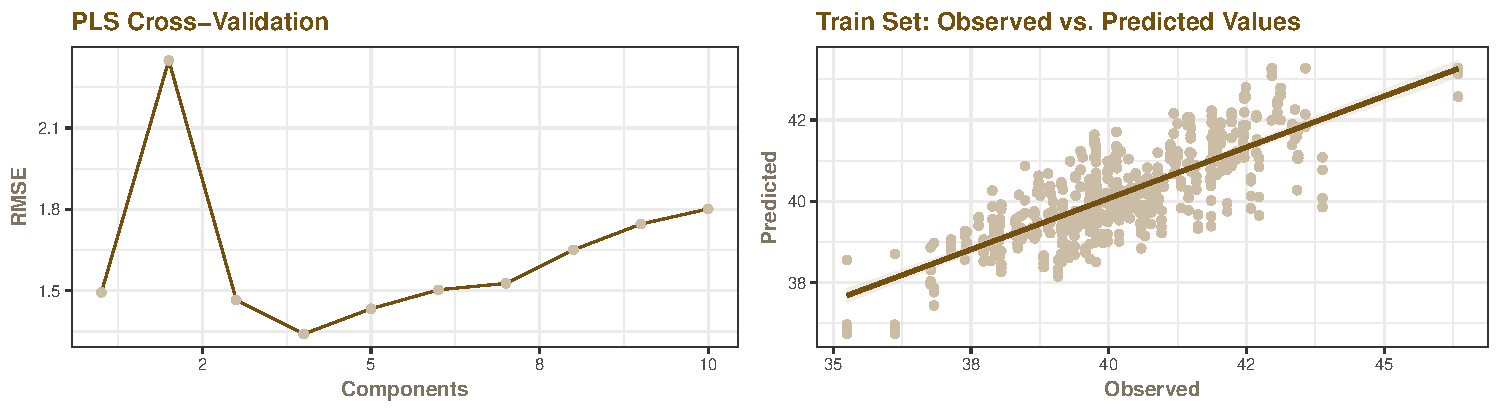
\includegraphics{Homework-Two2_files/figure-latex/kj-6.3c2-1.pdf}

\begin{subquestion}{(d).} Predict the response for the test set. What is the value of the performance metric and how does this compare with the resampled performance metric on the training set? 
\end{subquestion}

The \(R^2\) is greater for the test data, with 62\% of the data variance
explained. The RMSE has also dropped from the training results of 1.34
to the test result of 1.31. There is also a slight increased in the MAE.

\begin{table}[H]

\caption{\label{tab:kj-6.3d-1}PLS Performance Metrics on Test Subset}
\centering
\fontsize{8}{10}\selectfont
\begin{tabular}[t]{rrr}
\toprule
\textbf{RMSE} & \textbf{Rsquared} & \textbf{MAE}\\
\midrule
\rowcolor{gray!6}  1.3115 & 0.6183 & 1.0715\\
\bottomrule
\end{tabular}
\end{table}

Deviation in the line fitted to predicted vs.~observed values below
suggested that the selected linear model may not provide the best
predictions for \texttt{Yield}.

\begin{center}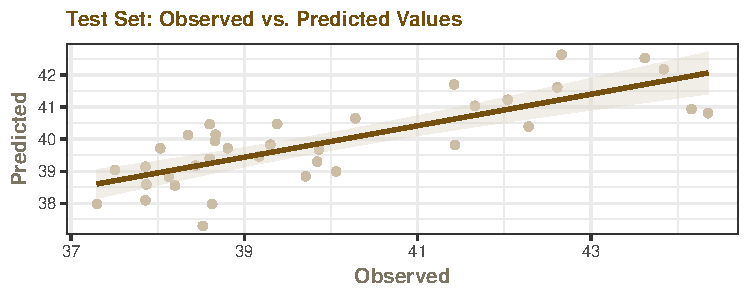
\includegraphics{Homework-Two2_files/figure-latex/kj-6.3d-2-1} \end{center}

\begin{subquestion}{(e).} Which predictors are most important in the model you have trained? Do either the biological or process predictors dominate the list? 
\end{subquestion}

VarImp identifies the variables by their importance.
\texttt{ManufacturingProcess32} is the most important predictor overall
as well as within the group of other Manufacturing Process variables.
\texttt{BiologicalMaterial06} ranked second and was the most important
variable amongst the BiologicalMaterial group. The variable importance
rankings are a mix; amonst the top 15 predictors, 7 are
BiologicalMaterials variabels and 8 are ManufacturingProcess variables.

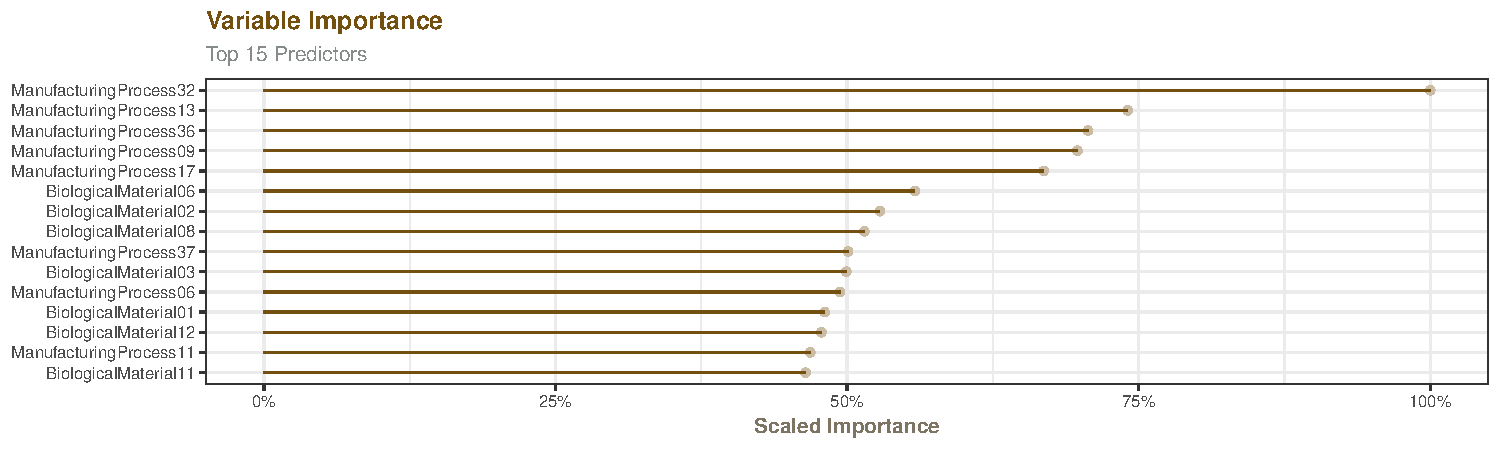
\includegraphics{Homework-Two2_files/figure-latex/kj-6.3e-1.pdf}

\begin{subquestion}{(f).} Explore the relationships between each of the top predictors and the response. How could this information be helpful in improving yield in future runs of the manufacturing process?
\end{subquestion}

A scatter plot helps to visualize relationship between our top five
important predictors against the response variable \texttt{Yield}. All
but \texttt{ManufacturingProcess32} show a moderate positive, linear
relationship with \texttt{Yield}.

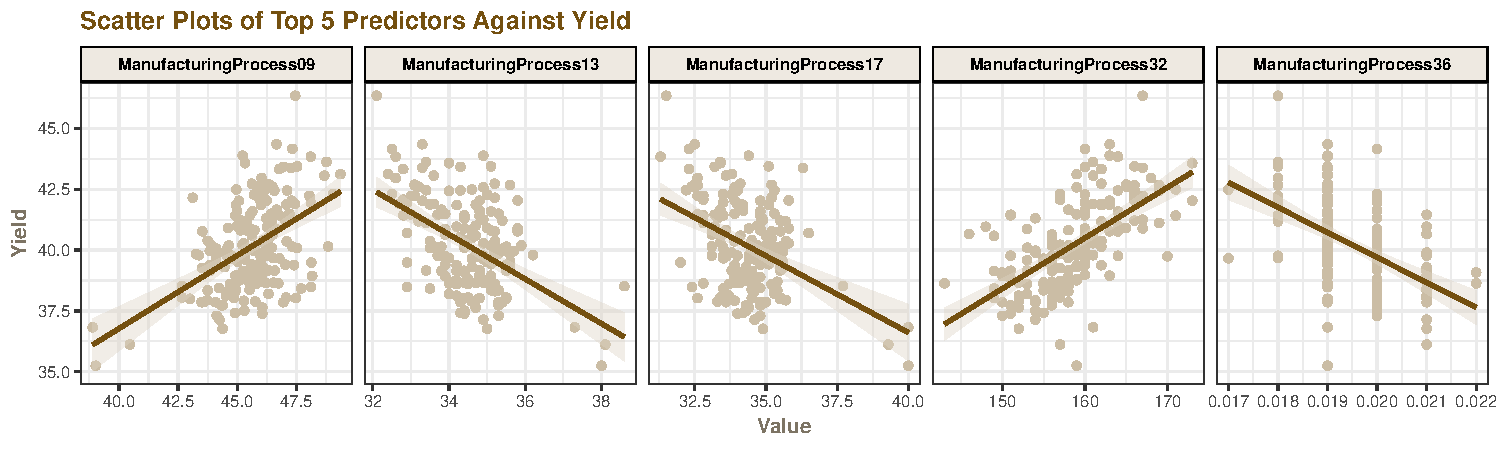
\includegraphics{Homework-Two2_files/figure-latex/kj-6.3f-1-1.pdf}

We further examined this relationship by analyzing the five response
variables most correlated with with the \texttt{Yield}, of which
\texttt{ManufacturingProcess32} was at the fore.

From a business point of view, the aim is to increase yield as this is
connected to revenue. While we don't have specific into the mechanics of
each manufacturing process, we can use this knowledge to adjust the
processes to emulate the highest yield outputs.

\begin{table}[H]

\caption{\label{tab:kj-6.3f-2}Variable Correlation with Yield}
\centering
\fontsize{8}{10}\selectfont
\begin{tabular}[t]{lr}
\toprule
\textbf{Variable} & \textbf{Yield}\\
\midrule
\rowcolor{gray!6}  ManufacturingProcess32 & 0.6083\\
ManufacturingProcess09 & 0.5035\\
\rowcolor{gray!6}  ManufacturingProcess17 & -0.4258\\
ManufacturingProcess36 & -0.5014\\
\rowcolor{gray!6}  ManufacturingProcess13 & -0.5037\\
\bottomrule
\end{tabular}
\end{table}

\chapter*{Assignment 2}\label{AS-2}
\addcontentsline{toc}{chapter}{Assignment 2}

\addcontentsline{toc}{subsection}{Kuhn and Johnson 7.2}

\begin{question}{Kuhn and Johnson 7.2}Friedman (1991) introduced several benchmark data sets create by simulation. One of these simulations used the following nonlinear equation to create data: $y = 10\text{sin}(\pi x_1 x_2)+20(x_3-0.5)^2+10x_4+5x_5+N(0\text{,} \sigma^2)$; where the $x$ values are random variables uniformly distributed between $[0, 1]$ (there are also 5 other non-informative variables also created in the simulation). 
\newline
The package `mlbench` contains a function called `mlbench.friedman1` that simulates these data. We convert the 'x' data from a matrix to a data frame. One reason is that this will give the columns names. The `testData` code creates a list with a vector 'y' and a matrix of predictors 'x'. It also simulates a large test set to estimate the true error rate with good precision: \end{question}

\begin{Shaded}
\begin{Highlighting}[]
\KeywordTok{set.seed}\NormalTok{(}\DecValTok{200}\NormalTok{)}
\NormalTok{trainingData <-}\StringTok{ }\KeywordTok{mlbench.friedman1}\NormalTok{(}\DecValTok{200}\NormalTok{, }\DataTypeTok{sd =} \DecValTok{1}\NormalTok{)}

\NormalTok{## We convert the 'x' data from a matrix to a data frame One}
\NormalTok{## reason is that this will give the columns names.}

\NormalTok{trainingData}\OperatorTok{$}\NormalTok{x <-}\StringTok{ }\KeywordTok{data.frame}\NormalTok{(trainingData}\OperatorTok{$}\NormalTok{x)}
\NormalTok{testData <-}\StringTok{ }\KeywordTok{mlbench.friedman1}\NormalTok{(}\DecValTok{5000}\NormalTok{, }\DataTypeTok{sd =} \DecValTok{1}\NormalTok{)}
\NormalTok{testData}\OperatorTok{$}\NormalTok{x <-}\StringTok{ }\KeywordTok{data.frame}\NormalTok{(testData}\OperatorTok{$}\NormalTok{x)}
\end{Highlighting}
\end{Shaded}

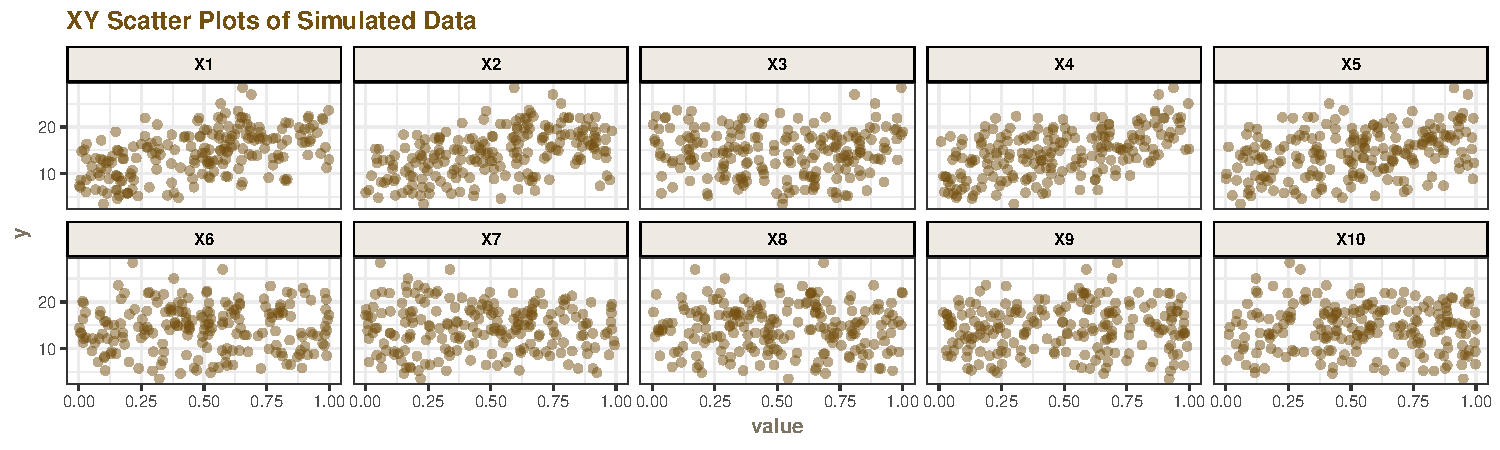
\includegraphics{Homework-Two2_files/figure-latex/kj-7.2-ex3-1.pdf}

\begin{subquestion}{(a).} Tune several models on these data. For example: 
\end{subquestion}

\begin{Shaded}
\begin{Highlighting}[]
\NormalTok{knnModel <-}\StringTok{ }\KeywordTok{train}\NormalTok{(}\DataTypeTok{x =}\NormalTok{ trainingData}\OperatorTok{$}\NormalTok{x, }\DataTypeTok{y =}\NormalTok{ trainingData}\OperatorTok{$}\NormalTok{y, }\DataTypeTok{method =} \StringTok{"knn"}\NormalTok{, }
    \DataTypeTok{preProc =} \KeywordTok{c}\NormalTok{(}\StringTok{"center"}\NormalTok{, }\StringTok{"scale"}\NormalTok{), }\DataTypeTok{tuneLength =} \DecValTok{10}\NormalTok{)}
\NormalTok{knnModel}
\NormalTok{knnPred <-}\StringTok{ }\KeywordTok{predict}\NormalTok{(knnModel, }\DataTypeTok{newdata =}\NormalTok{ testData}\OperatorTok{$}\NormalTok{x)}
\KeywordTok{postResample}\NormalTok{(}\DataTypeTok{pred =}\NormalTok{ knnPred, }\DataTypeTok{obs =}\NormalTok{ testData}\OperatorTok{$}\NormalTok{y)}
\end{Highlighting}
\end{Shaded}

\subsection{Model 1-MARS Regression:}\label{model-1-mars-regression}

MARS (Multivariate Adaptive Regression Splines) is a non-parametric
regression technique that automatically captures non-linearity and
interaction between predictors. The basic MARS model takes the following
form:

\[
\overset { \wedge  }{ f } =\sum _{ i=1 }^{ k }{ { c }_{ i }{ B }_{ i }(x) } 
\]

The model computes the sum of basis functions \(B\) multiplied by
constant coefficients \(C\). The basis function can either be a
constant, a hinge function, or a product of hinge functions. By
definition, a hinge function is a piecewise function that converges at a
point known as a knot.

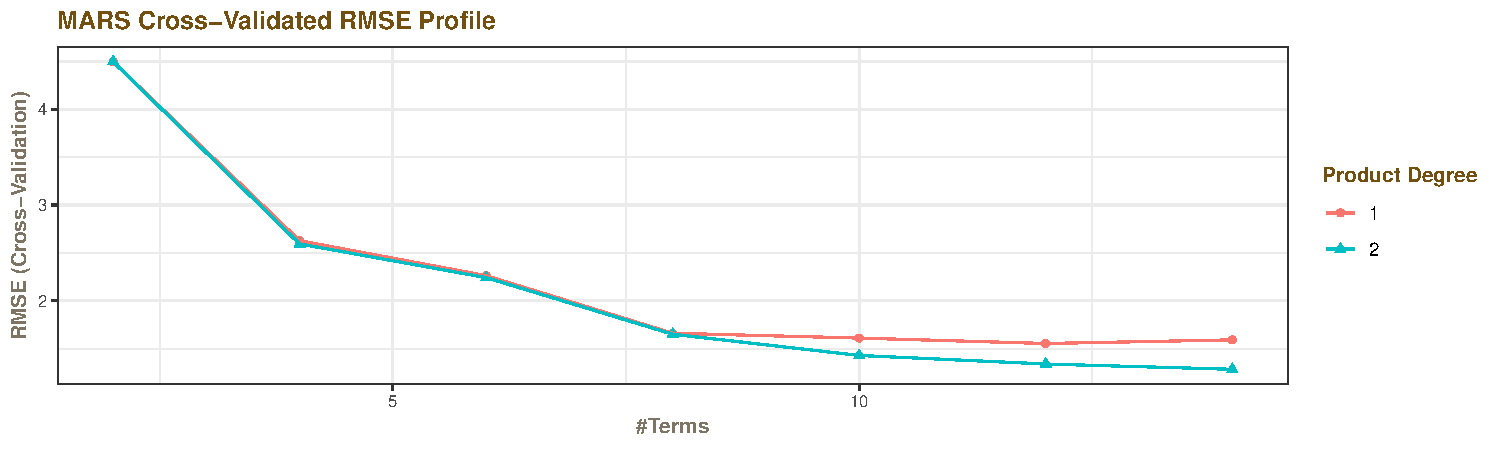
\includegraphics{Homework-Two2_files/figure-latex/kj-7.2-1-1.pdf}

\subsection{Model 2 SVM:}\label{model-2-svm}

SVM (Support Vector Machies) is a method that can be applied to
classification and regression tasks. SVM creates a hyperplane in n
dimensional space which acts as a margin-maximizing classification
boundary, either linear or nonlinear. This boundary classifies
information from a feature space.

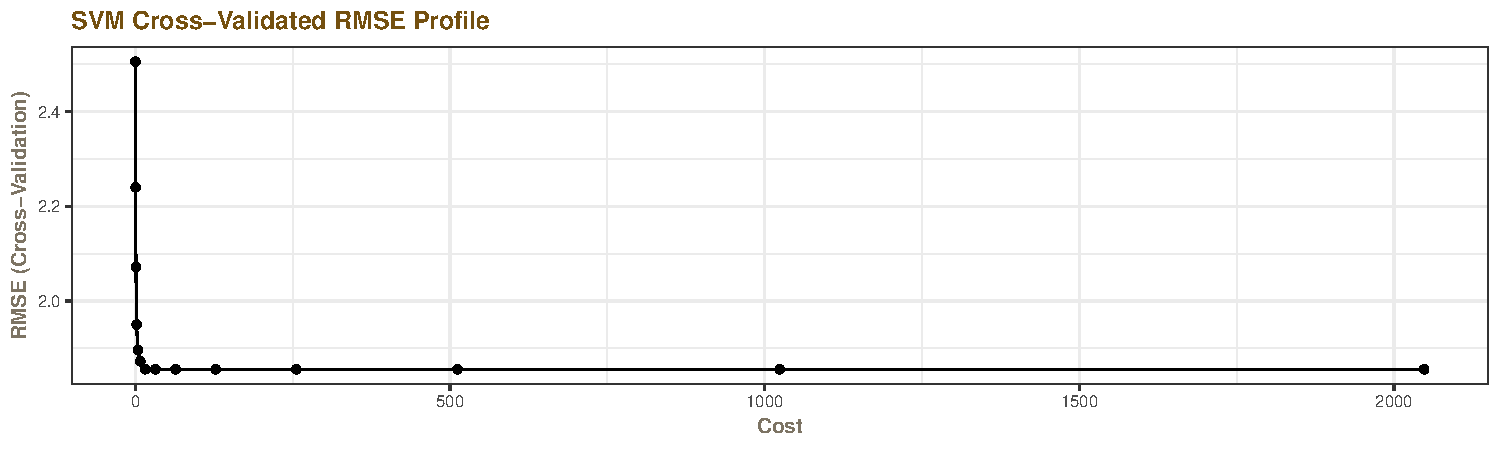
\includegraphics{Homework-Two2_files/figure-latex/kj-7.2-2-1.pdf}

\subsection{Model 3 NNET:}\label{model-3-nnet}

NNET (Neural Networks) is a method inspired by biological neuron
systems. It uses a system of nodes that parallel the way neurons work,
and is ideal for capturing non-linear relationships that would otherwise
be complicated in most multiple linear regression models. NNET evolves
internally based on the calculated weights of each input. The basic
structure is shown below:

\[
Y=\sum { (weight\quad *\quad input)\quad +\quad bias } 
\]

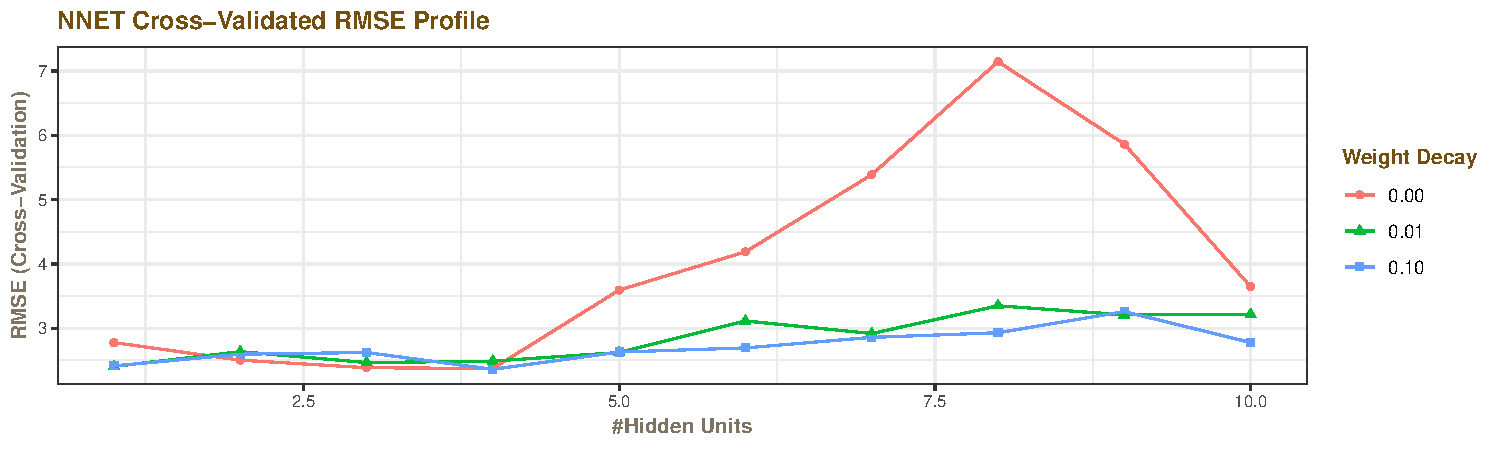
\includegraphics{Homework-Two2_files/figure-latex/kj-7.2-3-1.pdf}

\begin{subquestion}{(b).}
Which models appear to give the best performance? Does MARS select the informative predictors (those named X1-X5)?
\end{subquestion}

MARS appears to give the best performance based on RMSE, \(R^2\), and
MAE on test set. The performance metrics below show how other models
stack up against the MARS model.

\begin{table}[H]

\caption{\label{tab:unnamed-chunk-1}Model Performance}
\centering
\fontsize{8}{10}\selectfont
\begin{tabular}[t]{l|r|r|r}
\hline
\textbf{ } & \textbf{RMSE} & \textbf{RSquared} & \textbf{MAE}\\
\hline
\rowcolor{gray!6}  knnTrain & 3.5962 & 3.5962 & 3.5962\\
\hline
knnTest & 3.1751 & 0.6786 & 2.5443\\
\hline
\rowcolor{gray!6}  \rowcolor[HTML]{d9f2e6}  \textbf{MARSTrain} & \textbf{4.4979} & \textbf{0.9331} & \textbf{3.7465}\\
\hline
\rowcolor[HTML]{d9f2e6}  \textbf{MARSTest} & \textbf{1.1723} & \textbf{0.9449} & \textbf{0.9325}\\
\hline
\rowcolor{gray!6}  SVMTrain & 2.5054 & 0.8600 & 1.9897\\
\hline
SVMTest & 2.0702 & 0.8262 & 1.5725\\
\hline
\rowcolor{gray!6}  NNETTrain & 7.1443 & 0.7829 & 4.0248\\
\hline
NNETTest & 2.2434 & 0.8042 & 1.6997\\
\hline
\end{tabular}
\end{table}

The chart below demonstrates that variables \texttt{X1} through
\texttt{X5} are all important, with \texttt{X1} the most important. It
is very likely that the lack of contribution from variables \texttt{X6}
through \texttt{X10} bolster the models \(R^2\) and RMSE performance,
and that noise from these variables did not reduce the predictive
strength of this model as it does in small quantities in the other three
models.

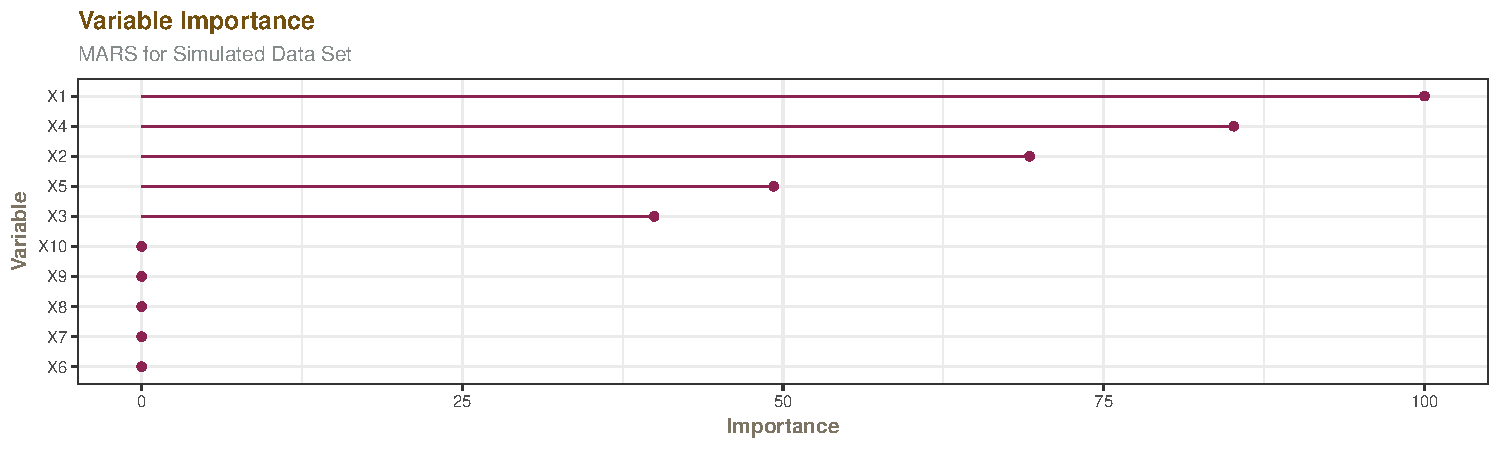
\includegraphics{Homework-Two2_files/figure-latex/kj-7.2-4b-1.pdf}

\addcontentsline{toc}{subsection}{Kuhn and Johnson 7.5}

\begin{question}{Kuhn and Johnson 7.5}
Exercise 6.3 describes data for a chemical manufacturing process. Use the same data imputation, data splitting, and pre-processing steps as before and train several nonlinear regression models.
\end{question}

We prepared data identically as in 6.3, imputing, removing near zero
variance features, and preproecessing. Please refer to 6.3 for a more
detailed look at the EDA involved with this data set.

We tuned KNN, NNET, MARS, and SVM models using specifications from the
textbook.

\begin{subquestion}{(a).}
Which nonlinear regression model gives the optimal resampling and test set performance? 
\end{subquestion}

SVM using a radial basis kernel outperformed the other models across all
performance metrics, followed by MARS regression. In part b, we will
address what variables are dominant in our SVM model.

\begin{table}[H]

\caption{\label{tab:unnamed-chunk-1}Model Performance on ChemicalManufacturing Data}
\centering
\fontsize{8}{10}\selectfont
\begin{tabular}[t]{l|r|r|r}
\hline
\textbf{ } & \textbf{RMSE} & \textbf{RSquared} & \textbf{MAE}\\
\hline
\rowcolor{gray!6}  knnTrain & 1.4808 & 0.4340 & 1.1588\\
\hline
knnTest & 1.4414 & 0.5216 & 1.2076\\
\hline
\rowcolor{gray!6}  MARSTrain & 1.4473 & 0.6539 & 1.1317\\
\hline
MARSTest & 1.2657 & 0.5836 & 1.0164\\
\hline
\rowcolor{gray!6}  \rowcolor[HTML]{d9f2e6}  \textbf{SVMTrain} & \textbf{1.3613} & \textbf{0.6278} & \textbf{1.1264}\\
\hline
\rowcolor[HTML]{d9f2e6}  \textbf{SVMTest} & \textbf{1.1888} & \textbf{0.6533} & \textbf{0.9179}\\
\hline
\rowcolor{gray!6}  NNETTrain & 9.6023 & 0.3722 & 5.8435\\
\hline
NNETTest & 1.7301 & 0.4157 & 1.4542\\
\hline
\end{tabular}
\end{table}

\begin{subquestion}{(b).}
Which predictors are most important in the optimal nonlinear regression model? Do either the biological or process variables dominate the list? How do the top ten important predictors compare to the top ten predictors from the optimal linear model? 
\end{subquestion}

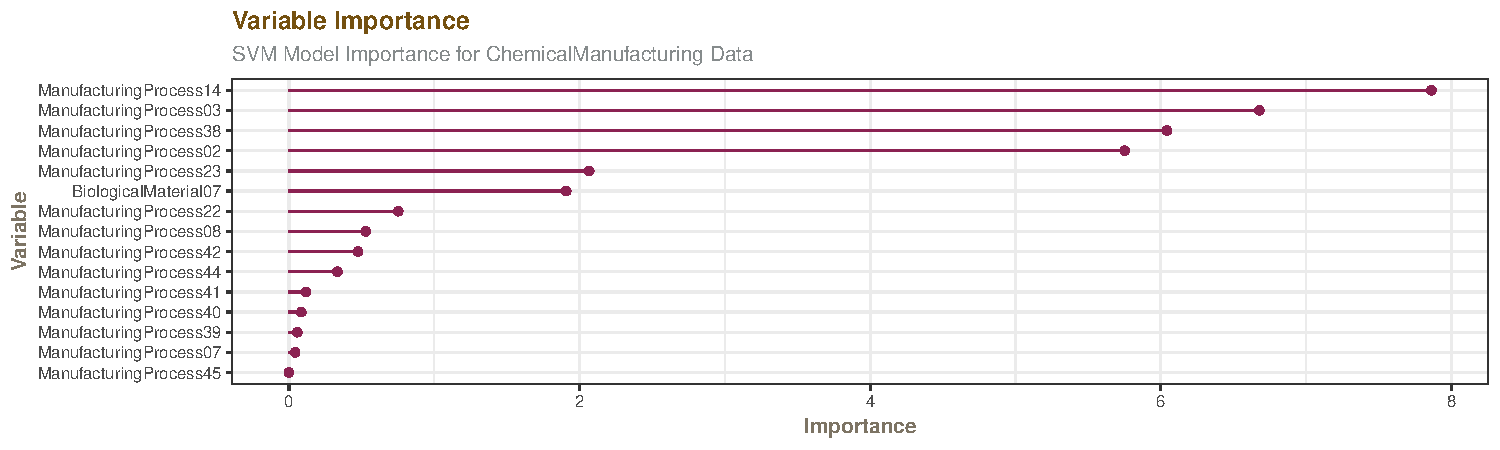
\includegraphics{Homework-Two2_files/figure-latex/kj-7.5b-1.pdf}

For the SVM model, \texttt{ManufacturingProcess} variables dominate the
importance rankings, with \texttt{ManufacturingProcess14} at the top. On
the other hand, for the linear model \texttt{ManufacturingProcess32} was
the most important variable with a number of \texttt{BiologicalProcess}
variables within the top 10.

\begin{subquestion}{(c).}
Explore the relationships between the top predictors and the response for the predictors that are unique to the optimal nonlinear regression model. Do these plots reveal intuition about the biological or process predictors and their relationship with yield?
\end{subquestion}

\begin{table}[H]

\caption{\label{tab:unnamed-chunk-1}Correlation}
\centering
\fontsize{8}{10}\selectfont
\begin{tabular}[t]{l|r}
\hline
VALUE & Yield\\
\hline
\rowcolor{gray!6}  Yield & 1.0000\\
\hline
ManufacturingProcess14 & -0.0103\\
\hline
\rowcolor{gray!6}  ManufacturingProcess38 & -0.0865\\
\hline
ManufacturingProcess03 & -0.1227\\
\hline
\rowcolor{gray!6}  ManufacturingProcess37 & -0.1593\\
\hline
ManufacturingProcess02 & -0.1947\\
\hline
\end{tabular}
\end{table}

We examined the top 5 predictors identified as the most important
variables before the importance measure dropped. There are some pretty
clear differences in the data which might explain both the overall poor
performance of the linear models as well as the improved significance of
\texttt{ManufacturingProcess} variables in the non-linear models.

Of the \texttt{ManfuacturingProcess} variables, they appear to be either
tight clusters or discrete values which predict an array of possible
\texttt{Yield}. This is directly opposed the definition of linearly
separable data base on earlier examination of correlation plots.

\chapter*{Assignment 3}\label{AS-3}
\addcontentsline{toc}{chapter}{Assignment 3}

\addcontentsline{toc}{subsection}{Kuhn and Johnson 8.1}

\begin{question}{Kuhn and Johnson 8.1} Recreate the simulated data from Exercise 7.2: \end{question}

\begin{subquestion}{(a).} Fit a random forest model to all of the predictors, then estimate the variable importance scores. Did the random forest model significantly use the uninformative predictors (V6-V10)?\end{subquestion}

The code for the RF model is provided by the textbook.

What is the code actually doing? We should dive into the theory. The
importance is calculated with the following formula:

\[
ni_j=W_{left(j)}C_{left(j)}-W_{right(j)}C_{right(j)}
\]

Let's deconstruct the theory. \(ni_j\) stands for node importance.
\(w_j\) is the weighted number of samples reaching node \(j\). \(c_j\)
is the impurity value of node \(j\). \(left(j)\) is the child node from
the left split on node \(j\) and \(right(j)\) is the child node from
right split on node \(j\). Once \(ni_j\) is calculated, the importance
for each variable on a decision tree is calculated with formula I.
Formula I is then normalized as shown as formula II. The final feature
importance is the average over all trees. We simply find the sum of the
features importance value and then divide by all trees T, shown in
formula III.

\[
I) \  fi_j \ =\frac{ (\sum_{j \ node \ split \ on \ i}) ni_j }{ ( \sum_{all \ nodes}) ni_k}\\
\]

\[
II) \  \parallel  fi_j  \parallel = \frac{(fi_j)}{\sum_{all \ features}fi_j} \\
\]

\[
III) \ RFfi_j= \frac{ ( \sum_{all \ trees})\parallel  fi_j \parallel}{T}
\]

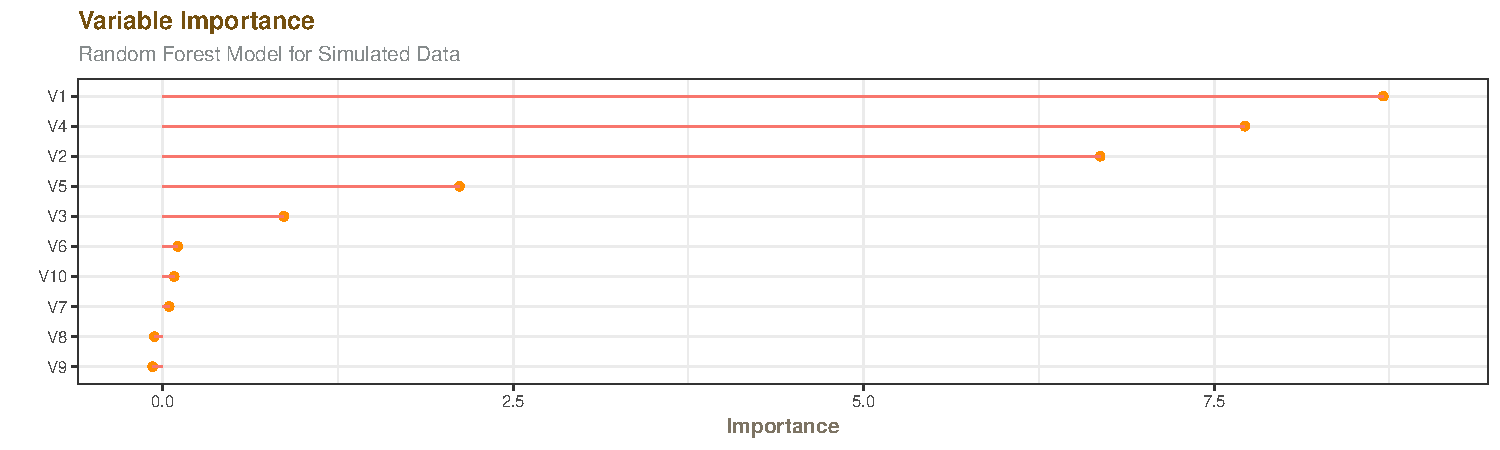
\includegraphics{Homework-Two2_files/figure-latex/kj-8.1a-1.pdf}

Variables \texttt{V6} through \texttt{V10} were some of the least
important variables, all with a measure less than 1. Variables
\texttt{V1} through \texttt{V5} were the most important, with variable
\texttt{V1} in the top spot.

\begin{subquestion}{(b).} Now add an additional predictor that is highly correlated with one of the informative predictors. Fit another random forest model to these data. Did the importance score for V1 change? What happens when you add another predictor that is also highly correlated with V1? For example:\end{subquestion}

We add a feature that has a strong correlation of .93 with existing
feature \texttt{V1} which we'll call \texttt{duplicate\ 1}

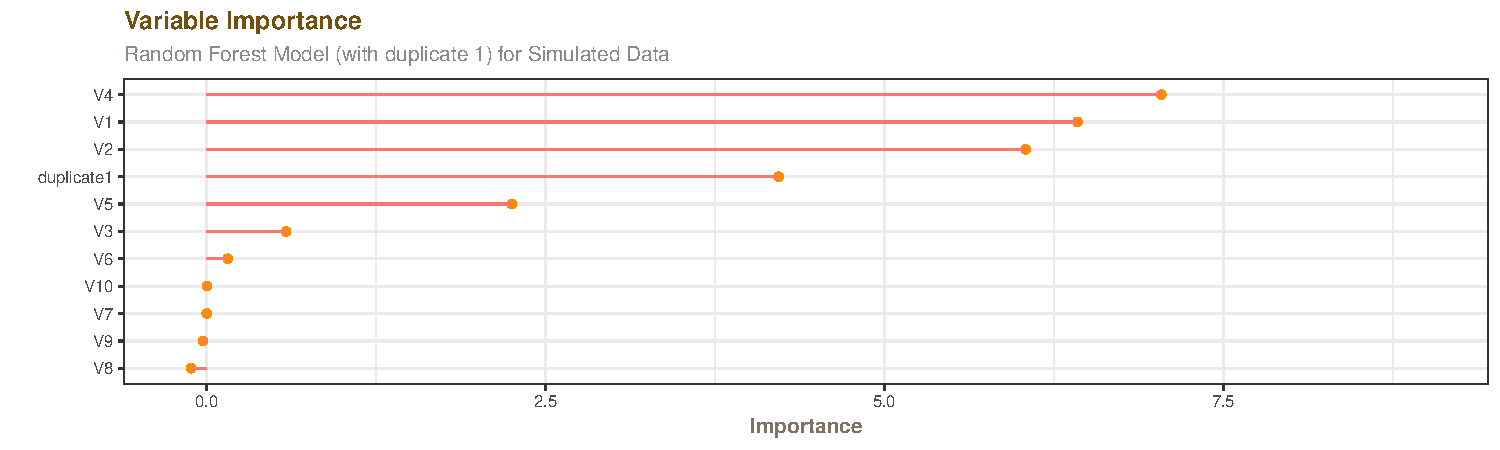
\includegraphics{Homework-Two2_files/figure-latex/kj-8.1b-1.pdf}

Note that \texttt{V1} decreased importance by roughly 2 measures.
\texttt{V4} is now the most important predictor. It looks like the
importance score for \texttt{V1} was partly absorbed by new predictor
which underestimates true importance of \texttt{V1} - the score sum of
\texttt{V1} and \texttt{duplicate1} are similar to the \texttt{V1} score
in (a). It makes sense as \texttt{duplicate1} contains almost the same
information as \texttt{V1}.

\begin{subquestion}{(c).} Use the `cforest` function in the party package to fit a random forest model using conditional inference trees. The party package function `varimp` can calculate predictor importance. The `conditional` argument of that function toggles between the traditional importance measure and the modified version described in Strobl et al. (2007). Do these importances show the same pattern as the traditional random forest model?\end{subquestion}

\begin{table}[H]

\caption{\label{tab:unnamed-chunk-1}Conditional vs Unconditional CForest Model: Variable Importance}
\centering
\fontsize{8}{10}\selectfont
\begin{tabular}[t]{l|r|r|r|r|r|r}
\hline
\textbf{features} & \textbf{RF} & \textbf{CF} & \textbf{RF.cor} & \textbf{CF.cor} & \textbf{CF.cond} & \textbf{CF.cor.cond}\\
\hline
\rowcolor{gray!6}  duplicate1 & NA & NA & 4.2213 & 7.6647 & NA & 1.3087\\
\hline
V1 & 8.7065 & 10.0562 & 6.4252 & 2.1014 & 3.3242 & 0.2776\\
\hline
\rowcolor{gray!6}  V2 & 6.6871 & 7.7244 & 6.0433 & 6.8085 & 4.7155 & 3.9022\\
\hline
V3 & 0.8648 & 0.0203 & 0.5894 & 0.0189 & 0.0223 & 0.0149\\
\hline
\rowcolor{gray!6}  V4 & 7.7190 & 10.6930 & 7.0444 & 9.8405 & 5.9425 & 5.5863\\
\hline
V5 & 2.1172 & 2.1893 & 2.2531 & 2.4539 & 0.7729 & 0.8364\\
\hline
\rowcolor{gray!6}  V6 & 0.1072 & 0.0335 & 0.1589 & 0.0398 & 0.0027 & -0.0023\\
\hline
V7 & 0.0465 & 0.0732 & 0.0042 & 0.0115 & 0.0188 & 0.0181\\
\hline
\rowcolor{gray!6}  V8 & -0.0588 & -0.0501 & -0.1113 & -0.0208 & -0.0015 & -0.0061\\
\hline
V9 & -0.0717 & -0.0265 & -0.0242 & -0.0293 & -0.0083 & -0.0099\\
\hline
\rowcolor{gray!6}  V10 & 0.0822 & 0.0060 & 0.0062 & -0.0153 & -0.0107 & 0.0102\\
\hline
\end{tabular}
\end{table}

We performed both \texttt{varimp(,\ conditional\ =\ T)} and
\texttt{varimp(,\ conditional\ =\ F)} to compare \texttt{varimp} of
\texttt{cforest} in terms of permutation importance and conditional
permutation importance.

\textbf{1. RF vs CF } Given that no correlated term is added, the
importance pattern is similar except for the fact that V4 is now the
most important feature in CF.

\textbf{2. RF vs CF (with correlated term added)} Given that the
correlated term is added, the importance score for \texttt{duplicate1}
is much smaller in CF. This is the pinpoint difference between
importance based on Gini coefficient (decision tree) and permutation
test using p-value (conditional inference tree).

\textbf{3. CF conditional vs CF with correlated term added and
conditional} When \texttt{conditional\ =\ T}, we perform conditional
permutation test for measuring feature importance instead. Note that
\texttt{duplicate1} has even smaller importance in \texttt{CF.cor.cond}
than in \texttt{CF.cor}. For \texttt{CF.cor.cond}, notice \texttt{V1}
became 3rd most important feature when it was 2nd most important for
\texttt{CF.cor}. This is because conditional permutation helps to
uncover the spurious correlation between \texttt{V1} and
\texttt{duplicate1}.

In summary, we learned that \texttt{CF} model surpresses the importance
score of \texttt{duplicate1}, which helps to maintain the importance of
\texttt{V1}. When \texttt{conditional\ =\ TRUE} in \texttt{varimp} for
\texttt{CF} model, the importance score of \texttt{duplicate1} is even
smaller.

\begin{subquestion}{(d).} Repeat this process with different tree models, such as boosted trees and Cubist. Does the same pattern occur?\end{subquestion}

Extracting the relative importance from a GBM object requires the use of
the native model summary. The summary returns the variable name along
with a measure of its influence on the target variable.

From the GBM tree, we can see \texttt{V4} is the most influential.
\texttt{V1} and correlated \texttt{duplicate1} are also much more
influential. \texttt{V6} through \texttt{V10} do not break the top half
of our list of influential variables.

\subsubsection{GBM Without Duplicate}\label{gbm-without-duplicate}

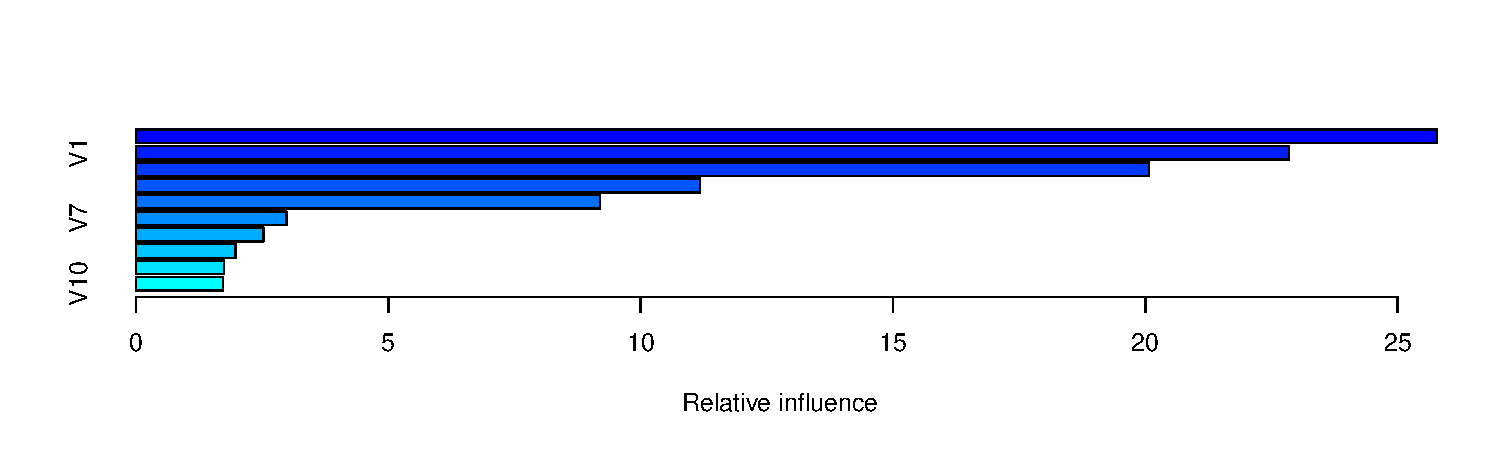
\includegraphics{Homework-Two2_files/figure-latex/kj-8.1d-1.pdf}

\begin{verbatim}
    var   rel.inf
V4   V4 25.780913
V1   V1 22.844642
V2   V2 20.070827
V5   V5 11.174466
V3   V3  9.191411
V7   V7  2.976852
V6   V6  2.523050
V9   V9  1.974093
V8   V8  1.742326
V10 V10  1.721421
\end{verbatim}

\subsubsection{GBM With Duplicate}\label{gbm-with-duplicate}

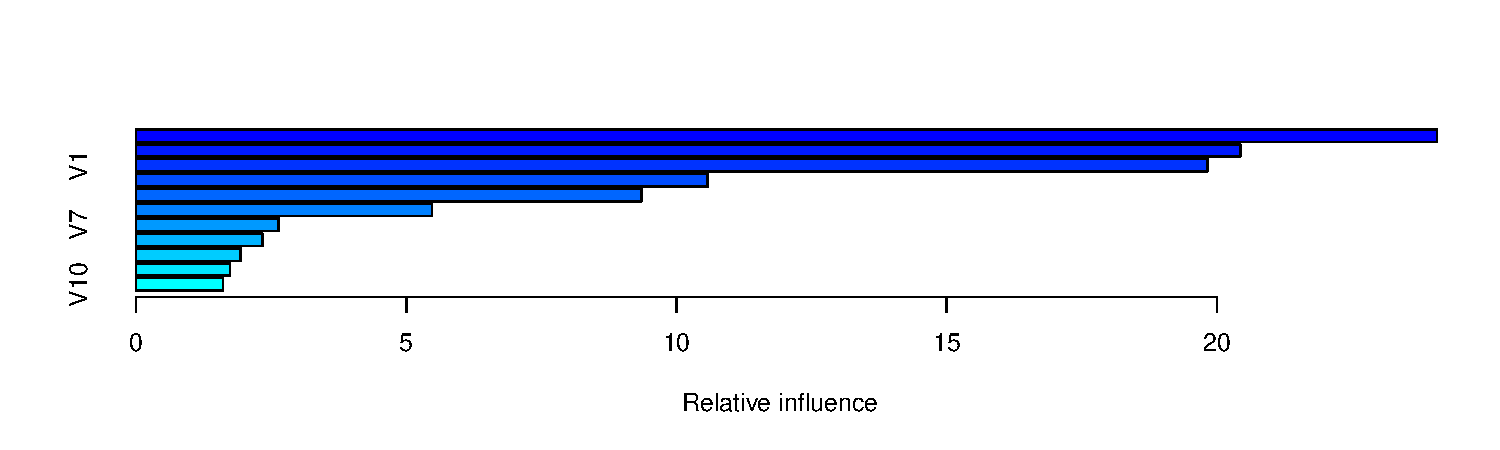
\includegraphics{Homework-Two2_files/figure-latex/kj-8.1da-1.pdf}

\begin{verbatim}
                  var   rel.inf
V4                 V4 24.072901
V2                 V2 20.432881
V1                 V1 19.823637
V5                 V5 10.574969
V3                 V3  9.353386
duplicate1 duplicate1  5.473609
V7                 V7  2.641898
V6                 V6  2.336609
V8                 V8  1.937914
V9                 V9  1.739826
V10               V10  1.612370
\end{verbatim}

The Cubist model is a rather unique variation on trees. Each leaf in the
tree - and each intermediate step between leafs - contains a linear
regression model. Every layer in the tree alters the predicitons used
within each leaf contained model. In other words, the selection of
predictors in leaf \(n\) is based on the previous splits. Predictions
are made via linear models on the terminal node.

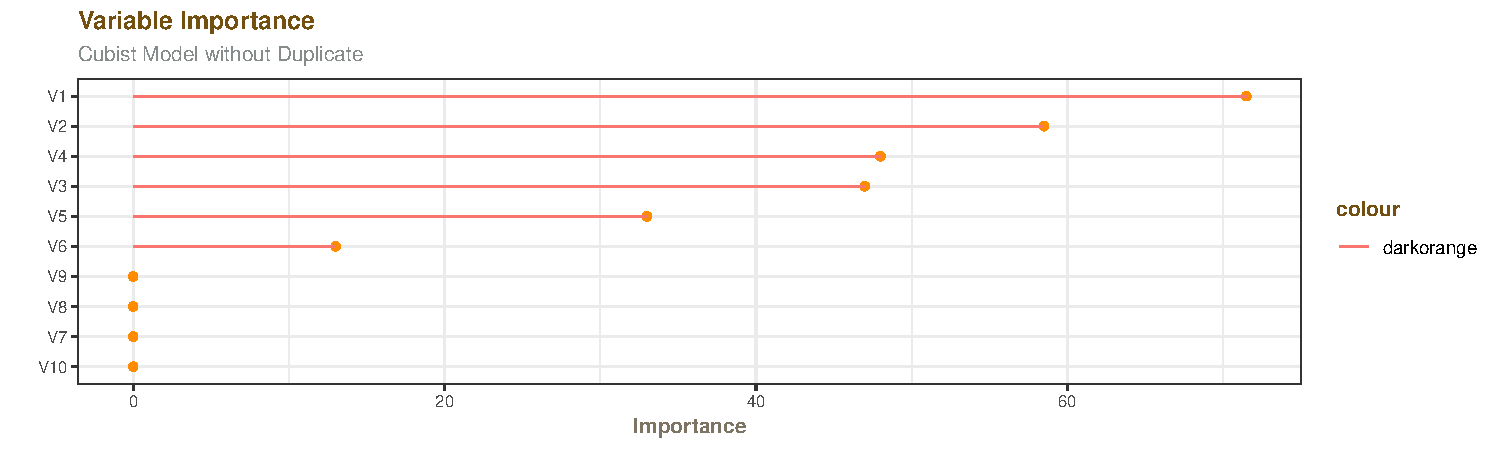
\includegraphics{Homework-Two2_files/figure-latex/kj-8.1db-1.pdf}
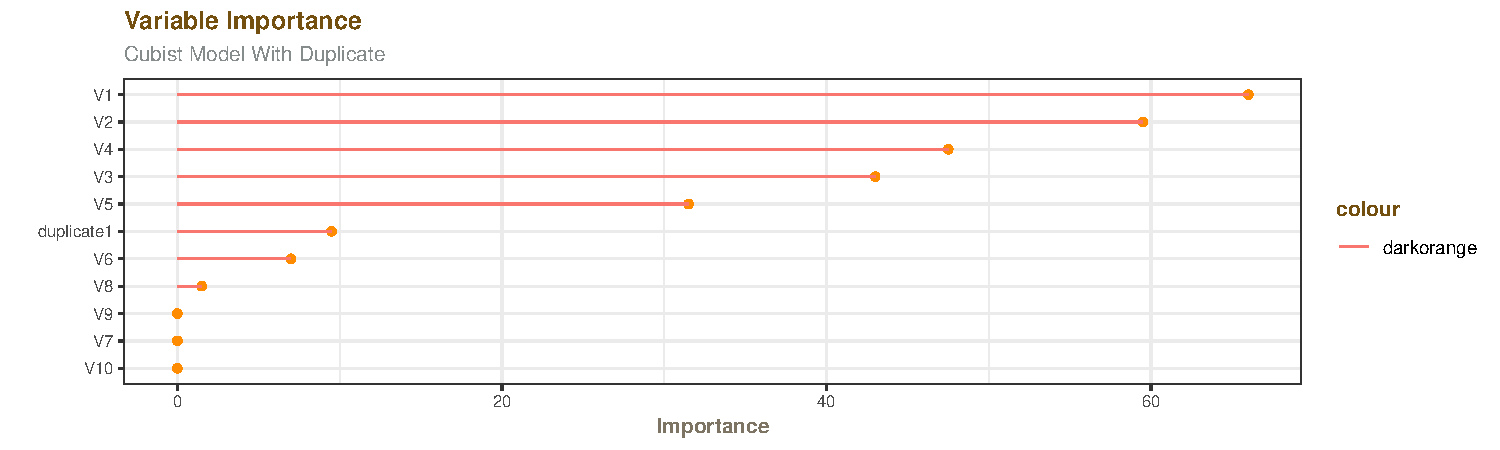
\includegraphics{Homework-Two2_files/figure-latex/kj-8.1db-2.pdf}

\addcontentsline{toc}{subsection}{Kuhn and Johnson 8.2}

\begin{question}{Kuhn and Johnson 8.2}Use a simulation to show tree bias with different granularities.\end{question}

Basic regression trees split predictor variables into small groups based
on response variable. According to the literature, ``predictors with a
higher number of distinct values are favored over more granular
predictors.''

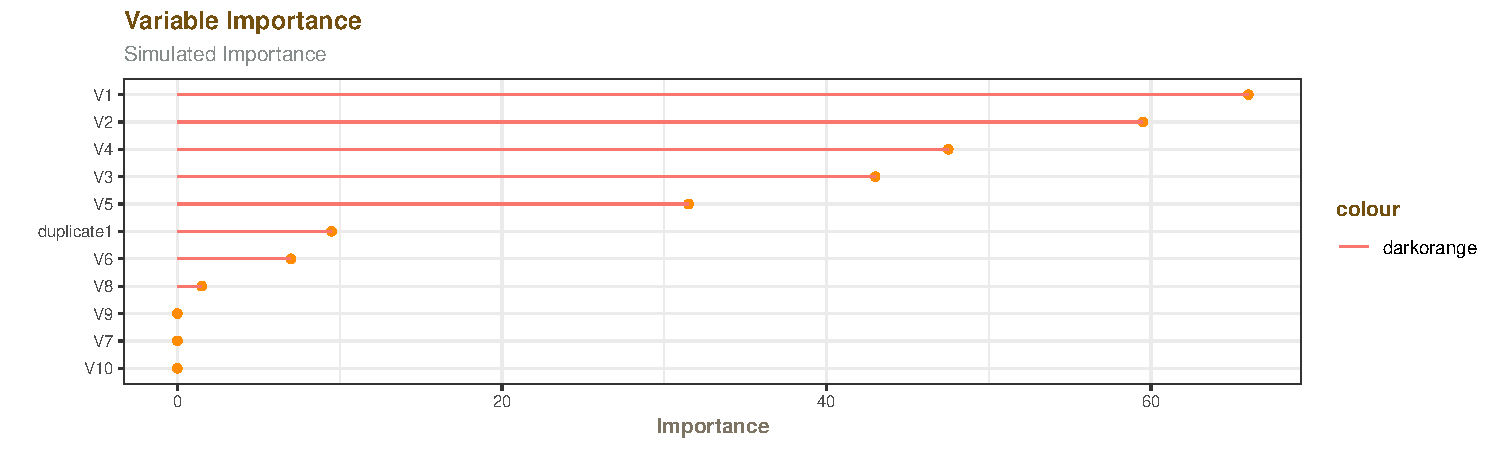
\includegraphics{Homework-Two2_files/figure-latex/kj-8.2-1.pdf}

\addcontentsline{toc}{subsection}{Kuhn and Johnson 8.3}

\begin{question}{Kuhn and Johnson 8.3} In stochastic gradient boosting the bagging fraction and learning rate will govern the construction of the trees as they are guided by the gradient. Although the optimal values of these parameters should be obtained through the tuning process, it is helpful to understand how the magnitudes of these parameters affect magnitudes of variable importance. Figure 8.24 provides the variable importance plots for boosting using two extreme values for the bagging fraction (0.1 and 0.9) and the learning rate (0.1 and 0.9) for the solubility data. The left-hand plot has both parameters set to 0.1, and the right-hand plot has both set to 0.9: \end{question}

\begin{subquestion}{(a).} Why does the model on the right focus its importance on just the first few of predictors, whereas the model on the left spreads importance across more predictors? \end{subquestion}

Because the model on the right has both high learning rates and high
bagging fractions, it does two things: first, it uses 90\% of the
variables in each tree, second, it uses 90\% of the error for a given
model.

Imagine a ten-variable model, with a bagging fraction of .9 every tree
would have nine of the ten trees in it and only one variable would be
different from the set of 9 trees in the first model each time. In this
case, most of the possible break-points would be the same from tree to
tree and different initial splits would only be possible when the
dominant variable is removed. As a result, these modles would likely
make the same first few decisions each time. Given that with a .9
learning rate 90\% of the error is added in from each tree, in addition
to consistently choosing from one or a few initial splits the models are
also maximizing the contributions of those splits.

Given these learning rates and bagging fractions, the trees contributing
to the Stochastic Boosted Tree in this example will make the same
decisions repeatedely, yielding very few unique decisions overall. Lack
of variation in initial choices means that the number of paths the
learning can take is limited, and with a high learning rate a core set
of variables is selected early on from the similarly built trees. In
essence, the model never has the opportunity to evaluate other possible
variables because the greediness of the model makes the same first few
choices every time.

\begin{subquestion}{(b).} Which model do you think would be more predictive of other samples?\end{subquestion}

The .9 / .9 model would likely overfit the training data, because the
variation in values within those most important variables may not
reflect the general population. This model will be tuned to choose from
sample members following the samples' distributions along the most
important features at the expense of recognizing potential splits in
other features which might be more common in the general population.

With a learning rate of .1 and a bagging fraction of .1, the left model
is more likely to build truly weak predictors, from smallers sets of
variables, consider more distinct breaking points, and therefore extend
better to wild data not fully described by the first few variables in
the importance summarise\_layers.

\begin{subquestion}{(c).} How would increasing interaction depth affect the slope of predictor importance for either model in Fig.8.24?\end{subquestion}

Increasing the tree depth would affect both models, but differently.

For the model with bagging fraction and learning rate equal to .1,
increasing the number of nodes in the tree would likely increase the
importance of less important variables, creating a less polynomial
slope. The reason for this is that making more decisions means giving
weight to the variables and values where those decisions are made.

For the model with bagging fraction and learning rate equal to .9,
increasing the depth would likely not change the slope of less important
lower variables, just adding a new variable or two to the top.

In this model with high bagging fraction and learning rate we will still
be making most of the same decisions from tree to tree. Increases in
importance will come from nodes added downstream, and these are likely
to be the same from tree to tree. As a result, you might find added
importance low on the scale for those variables upon which the new nodes
break, or for variables higher on the scale with a second or third
break. This might lead to a reshuffling of upper nodes and a slight
increase of one or two less important variables, but the overall slope
quickly going to zero will be constrained by the high bagging fraction
and learning rate.

\addcontentsline{toc}{subsection}{Kuhn and Johnson 8.7}

\begin{question}{Kuhn and Johnson 8.7}
Refer to Exercises 6.3 and 7.5 which describe a chemical manufacturing process. Use the same data imputation, data splitting, and pre-processing steps as before and train several tree-based models:
\end{question}

\begin{subquestion}{(a).} Which tree-based regression model gives the optimal resampling and test set performance? \end{subquestion}

\begin{table}[H]

\caption{\label{tab:unnamed-chunk-1}Tree Model Performance on ChemicalManufacturing Data}
\centering
\fontsize{8}{10}\selectfont
\begin{tabular}[t]{l|r|r|r}
\hline
\textbf{ } & \textbf{RMSE} & \textbf{RSquared} & \textbf{MAE}\\
\hline
\rowcolor{gray!6}  GBM & 1.4363 & 0.5957 & 1.1565\\
\hline
GBMTest & 1.1658 & 0.6654 & 0.9339\\
\hline
\rowcolor{gray!6}  RFTrain & 1.2430 & 0.5706 & 0.9350\\
\hline
RFTest & 1.2145 & 0.6674 & 0.9638\\
\hline
\rowcolor{gray!6}  \rowcolor[HTML]{d9f2e6}  \textbf{CubistTrain} & \textbf{0.9882} & \textbf{0.7519} & \textbf{0.7678}\\
\hline
\rowcolor[HTML]{d9f2e6}  \textbf{CubistTest} & \textbf{1.0700} & \textbf{0.7074} & \textbf{0.8232}\\
\hline
\end{tabular}
\end{table}

The Cubist model is the optimal based on the \(R^2\) value. Cubist has a
lower \texttt{RMSE} both on the train and test data across the different
selected tree models.

\begin{subquestion}{(b).} Which predictors are most important in the optimal tree-based regression model? Do either the biological or process variables dominate the list? How do the top 10 important predictors compare to the top 10 predictors from the optimal linear and nonlinear models?\end{subquestion}

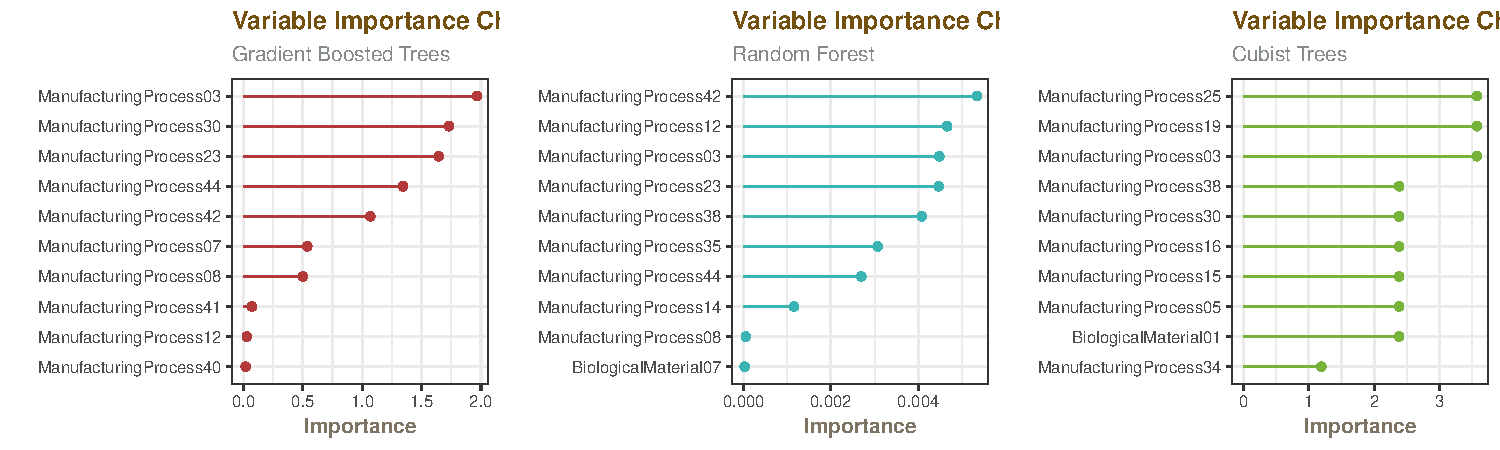
\includegraphics{Homework-Two2_files/figure-latex/kj-8.7b-1.pdf}

In all the models the \texttt{ManufacturingProcess} variables dominate
the list, with slight differences in position and influence.

Comparing the top 10 variables in each model reveals some strong
differences. The Boosted Tree model sees a rather linear drop-off of
importance through a list of exclusively \texttt{ManufacturingProcess}
variables. The Random Forest model falls off slower in the first five
variables but becomes rapidly linear; all but the last are
\texttt{ManufacturingProcess} variables. The Cubist tree depreciates
differently at seemingly discrete levels; other than the first and last
variables, all are \texttt{ManufacturingProcess} variables.

\begin{subquestion}{(c).} Plot the optimal single tree with the distribution of yield in the terminal nodes. Does this view of the data provide additional knowledge about the biological or process predictors and their relationship with yield?\end{subquestion}

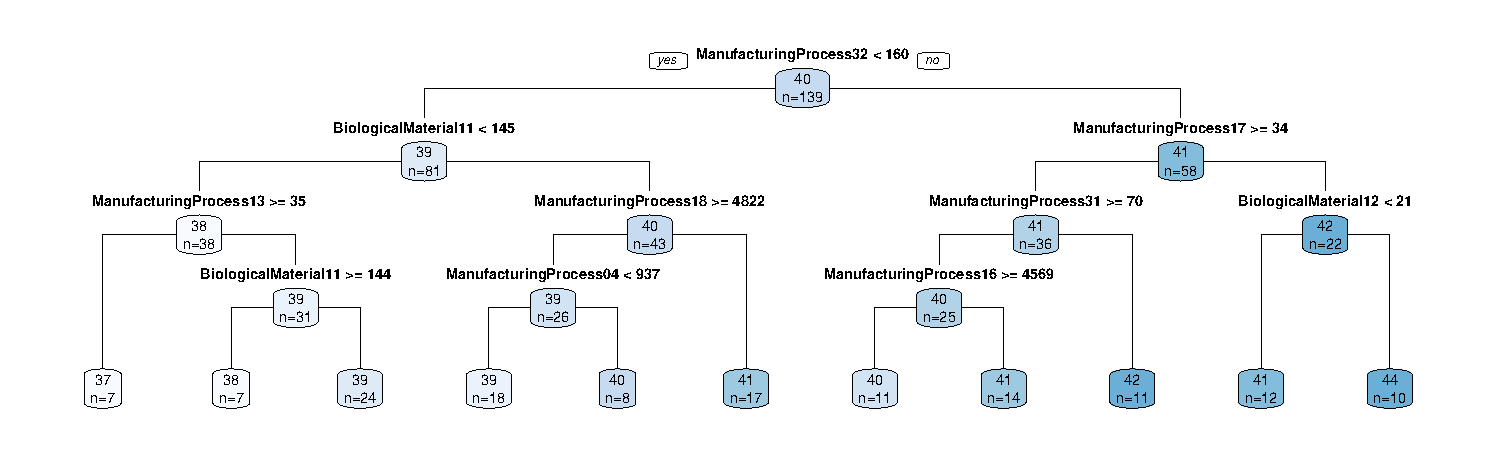
\includegraphics{Homework-Two2_files/figure-latex/kj-8.7c-1.pdf}

Based on this regression tree, the differences between
\texttt{ManufacturingProcess} and \texttt{BiologicalMaterials} is that
the formerdifferentiate more observations at each break and so break
first. While this increases node purity quickly, the final decisions
seem to be based rather wholly on the latter variables. Accordingly,
looking only at \texttt{ManufacturingProcess} variables or prunning too
early could lead to overfitting.

\chapter*{R Script}\label{R-Script}
\addcontentsline{toc}{chapter}{R Script}

\begin{Shaded}
\begin{Highlighting}[]
\NormalTok{## Dependencies}
\CommentTok{# SOURCE DEFAULT SETTINGS}
\NormalTok{### UNIVERSAL DATA SOURCING & DEFAULT SETTINGS FOR PROJECT}
\KeywordTok{library}\NormalTok{(knitr)}
\KeywordTok{library}\NormalTok{(kableExtra)}
\KeywordTok{library}\NormalTok{(default)}
\KeywordTok{library}\NormalTok{(ggplot2)}
\KeywordTok{library}\NormalTok{(easypackages)}
\KeywordTok{library}\NormalTok{(formatR)}

\CommentTok{# Set default augments for code chunks}
\NormalTok{knitr}\OperatorTok{::}\NormalTok{opts_chunk}\OperatorTok{$}\KeywordTok{set}\NormalTok{(}\DataTypeTok{echo =}\NormalTok{ F, }\DataTypeTok{message=}\NormalTok{F, }\DataTypeTok{warning=}\NormalTok{F, }\DataTypeTok{error=}\NormalTok{F, }\DataTypeTok{comment=}\OtherTok{NA}\NormalTok{, }\DataTypeTok{tidy=}\NormalTok{T, }\DataTypeTok{tidy.opts=}\KeywordTok{list}\NormalTok{(}\DataTypeTok{width.cutoff=}\DecValTok{60}\NormalTok{), }\DataTypeTok{fig.width=}\DecValTok{10}\NormalTok{, }\DataTypeTok{fig.height =} \DecValTok{3}\NormalTok{)}

\CommentTok{# Set default augments for `kable()` }
\KeywordTok{default}\NormalTok{(kable) <-}\StringTok{ }\KeywordTok{list}\NormalTok{(}\DataTypeTok{format=}\StringTok{"latex"}\NormalTok{, }\DataTypeTok{digits=}\DecValTok{4}\NormalTok{)}

\CommentTok{# Set default augments for `kable_styling()` }
\KeywordTok{default}\NormalTok{(kable_styling)  <-}\StringTok{ }\KeywordTok{list}\NormalTok{(}\DataTypeTok{latex_options =} \KeywordTok{c}\NormalTok{(}\StringTok{"HOLD_position"}\NormalTok{, }\StringTok{"striped"}\NormalTok{), }\DataTypeTok{font_size=}\DecValTok{8}\NormalTok{)}
\KeywordTok{default}\NormalTok{(row_spec) <-}\StringTok{ }\KeywordTok{list}\NormalTok{(}\DataTypeTok{row=}\DecValTok{0}\NormalTok{, }\DataTypeTok{bold=}\NormalTok{T)}

\CommentTok{# Set default augments for ggplot2 `theme()`}
\KeywordTok{default}\NormalTok{(theme) <-}\StringTok{ }\KeywordTok{list}\NormalTok{(}\DataTypeTok{axis.text.x =} \KeywordTok{element_text}\NormalTok{(}\DataTypeTok{size=}\DecValTok{8}\NormalTok{),}
                       \DataTypeTok{axis.text.y =} \KeywordTok{element_text}\NormalTok{(}\DataTypeTok{size=}\DecValTok{8}\NormalTok{),}
                       \DataTypeTok{axis.title.x =} \KeywordTok{element_text}\NormalTok{(}\DataTypeTok{color=}\StringTok{"#7d7464"}\NormalTok{, }\DataTypeTok{face=}\StringTok{"bold"}\NormalTok{, }\DataTypeTok{size=}\DecValTok{10}\NormalTok{, }\DataTypeTok{angle =} \DecValTok{0}\NormalTok{, }\DataTypeTok{hjust =} \OtherTok{NULL}\NormalTok{),}
                       \DataTypeTok{axis.title.y =} \KeywordTok{element_text}\NormalTok{(}\DataTypeTok{color=}\StringTok{"#7d7464"}\NormalTok{, }\DataTypeTok{face=}\StringTok{"bold"}\NormalTok{, }\DataTypeTok{size=}\DecValTok{10}\NormalTok{),}
                       \DataTypeTok{plot.title =} \KeywordTok{element_text}\NormalTok{(}\DataTypeTok{color=}\StringTok{"#745010"}\NormalTok{, }\DataTypeTok{size=}\DecValTok{12}\NormalTok{, }\DataTypeTok{face=}\StringTok{"bold"}\NormalTok{),}
                       \DataTypeTok{plot.subtitle =}\NormalTok{ (}\KeywordTok{element_text}\NormalTok{(}\DataTypeTok{size=}\DecValTok{10}\NormalTok{, }\DataTypeTok{color=}\StringTok{"#868b8c"}\NormalTok{)),}
                       \DataTypeTok{legend.title =}\NormalTok{ (}\KeywordTok{element_text}\NormalTok{(}\DataTypeTok{size=}\DecValTok{10}\NormalTok{, }\DataTypeTok{color=}\StringTok{"#745010"}\NormalTok{, }\DataTypeTok{face=}\StringTok{"bold"}\NormalTok{)),}
                       \DataTypeTok{strip.background =} \KeywordTok{element_rect}\NormalTok{(}\DataTypeTok{color=}\StringTok{"#000000"}\NormalTok{, }
                                                       \DataTypeTok{fill=}\StringTok{"#eee9e1"}\NormalTok{, }\DataTypeTok{size=}\NormalTok{.}\DecValTok{75}\NormalTok{,}\DataTypeTok{linetype=}\StringTok{"solid"}\NormalTok{),}
                       \DataTypeTok{strip.text.x =} \KeywordTok{element_text}\NormalTok{(}\DataTypeTok{size =} \DecValTok{8}\NormalTok{, }\DataTypeTok{color =} \StringTok{"#000000"}\NormalTok{, }\DataTypeTok{face=}\StringTok{"bold"}\NormalTok{))}

\CommentTok{# SOURCE HW ANSWERS}

\NormalTok{## Ensure constistent variable naming convention per question}
\NormalTok{## Look out for duplicate variable names between questions}

\CommentTok{# DEPENDENCIES}


\CommentTok{# Predicitve Modeling}
\KeywordTok{libraries}\NormalTok{(}\StringTok{'AppliedPredictiveModeling'}\NormalTok{, }\StringTok{'mice'}\NormalTok{,}\StringTok{'caret'}\NormalTok{, }\StringTok{'tidyverse'}\NormalTok{,}\StringTok{'impute'}\NormalTok{,}\StringTok{'pls'}\NormalTok{,}\StringTok{'caTools'}\NormalTok{,}\StringTok{'mlbench'}\NormalTok{,}\StringTok{'randomForest'}\NormalTok{,}\StringTok{'party'}\NormalTok{,}\StringTok{'gbm'}\NormalTok{,}\StringTok{'Cubist'}\NormalTok{,}\StringTok{'rpart'}\NormalTok{)}
\CommentTok{# Formatting Libraries}
\KeywordTok{libraries}\NormalTok{(}\StringTok{'default'}\NormalTok{, }\StringTok{'knitr'}\NormalTok{, }\StringTok{'kableExtra'}\NormalTok{,}\StringTok{'gridExtra'}\NormalTok{,}\StringTok{'sqldf'}\NormalTok{)}
\CommentTok{# Plotting Libraries}
\KeywordTok{libraries}\NormalTok{(}\StringTok{'ggplot2'}\NormalTok{, }\StringTok{'grid'}\NormalTok{, }\StringTok{'ggfortify'}\NormalTok{,}\StringTok{'rpart.plot'}\NormalTok{)}


\CommentTok{# Data Wrangling }
\KeywordTok{library}\NormalTok{(AppliedPredictiveModeling); }\KeywordTok{library}\NormalTok{(mice); }\KeywordTok{library}\NormalTok{(caret); }\KeywordTok{library}\NormalTok{(tidyverse); }\KeywordTok{library}\NormalTok{(pls); }\KeywordTok{library}\NormalTok{(caTools); }\KeywordTok{library}\NormalTok{(mlbench); }\KeywordTok{library}\NormalTok{(stringr);}
\CommentTok{# Formatting}
\KeywordTok{library}\NormalTok{(default); }\KeywordTok{library}\NormalTok{(knitr); }\KeywordTok{library}\NormalTok{(kableExtra); }
\CommentTok{# Plotting}
\KeywordTok{library}\NormalTok{(ggplot2); }\KeywordTok{library}\NormalTok{(grid); }\KeywordTok{library}\NormalTok{(ggfortify)}

\CommentTok{# THEME COLORS}
\NormalTok{dark_gold <-}\StringTok{ "#745010"}
\NormalTok{medium_gold <-}\StringTok{ "#cbbda5"}
\NormalTok{light_gold <-}\StringTok{ "#dcd3c3"}

\CommentTok{# SET SEED}

\KeywordTok{set.seed}\NormalTok{(}\DecValTok{58677}\NormalTok{)}

\CommentTok{# ASSIGNMENT 1 }
\CommentTok{# KJ 6.3}
\KeywordTok{data}\NormalTok{(}\StringTok{"ChemicalManufacturingProcess"}\NormalTok{)}

\CommentTok{# (6.3a) }
\NormalTok{Plt_CMP.Yield <-}\KeywordTok{ggplot}\NormalTok{(ChemicalManufacturingProcess, }\KeywordTok{aes}\NormalTok{(}\DataTypeTok{x =}\NormalTok{ Yield))}\OperatorTok{+}
\StringTok{  }\KeywordTok{geom_histogram}\NormalTok{(}\DataTypeTok{color=}\NormalTok{dark_gold, }\DataTypeTok{fill =}\NormalTok{ light_gold)}\OperatorTok{+}
\StringTok{  }\KeywordTok{scale_x_continuous}\NormalTok{(}\DataTypeTok{labels =}\NormalTok{ scales}\OperatorTok{::}\KeywordTok{number_format}\NormalTok{(}\DataTypeTok{accuracy =}\NormalTok{ .}\DecValTok{1}\NormalTok{))}\OperatorTok{+}
\StringTok{  }\KeywordTok{labs}\NormalTok{(}\DataTypeTok{title=}\StringTok{"Distribution of Yield"}\NormalTok{) }\OperatorTok{+}
\StringTok{  }\KeywordTok{theme_bw}\NormalTok{()}\OperatorTok{+}\KeywordTok{theme}\NormalTok{(}\DataTypeTok{plot.title =} \KeywordTok{element_text}\NormalTok{(}\DataTypeTok{color=}\StringTok{"#745010"}\NormalTok{, }\DataTypeTok{size=}\DecValTok{10}\NormalTok{, }\DataTypeTok{face=}\StringTok{"bold"}\NormalTok{), }\DataTypeTok{axis.title.y =} \KeywordTok{element_blank}\NormalTok{())}

\CommentTok{# (6.3b) }

\CommentTok{# Total NA Values}
\CommentTok{#na_table<- table(is.na(ChemicalManufacturingProcess))}
\NormalTok{CMP_na <-}\StringTok{ }\NormalTok{ChemicalManufacturingProcess }\OperatorTok\StringTok{ }\KeywordTok{select}\NormalTok{(}\OperatorTok{-}\NormalTok{Yield) }\OperatorTok\StringTok{ }\KeywordTok{summarise_all}\NormalTok{(}\KeywordTok{funs}\NormalTok{(}\KeywordTok{sum}\NormalTok{(}\KeywordTok{is.na}\NormalTok{(.)))) }\OperatorTok\StringTok{ }\KeywordTok{t}\NormalTok{() }\OperatorTok\StringTok{ }\KeywordTok{as.data.frame}\NormalTok{() }\OperatorTok\StringTok{ }\KeywordTok{rownames_to_column}\NormalTok{(}\StringTok{"Predictor"}\NormalTok{) }\OperatorTok\StringTok{ }\KeywordTok{filter}\NormalTok{(V1 }\OperatorTok{>}\StringTok{ }\DecValTok{0}\NormalTok{) }\OperatorTok\StringTok{ }\KeywordTok{arrange}\NormalTok{(}\KeywordTok{desc}\NormalTok{(V1)) }\OperatorTok\StringTok{ }\KeywordTok{rename}\NormalTok{(}\DataTypeTok{n=}\NormalTok{V1)}
\NormalTok{CMP_na_left <-CMP_na }\OperatorTok\StringTok{ }\KeywordTok{slice}\NormalTok{(}\DecValTok{1}\OperatorTok{:}\DecValTok{14}\NormalTok{); CMP_na_right <-}\StringTok{ }\NormalTok{CMP_na }\OperatorTok\StringTok{ }\KeywordTok{slice}\NormalTok{(}\DecValTok{15}\OperatorTok{:}\DecValTok{28}\NormalTok{); CMP.total_na <-}\StringTok{ }\KeywordTok{cbind}\NormalTok{(CMP_na_left, }\StringTok{`}\DataTypeTok{ }\StringTok{`}\NormalTok{=}\StringTok{" "}\NormalTok{, CMP_na_right)}

\CommentTok{# use mice w/ default settings to impute missing data}
\NormalTok{miceImp <-}\StringTok{ }\KeywordTok{mice}\NormalTok{(ChemicalManufacturingProcess, }\DataTypeTok{printFlag =} \OtherTok{FALSE}\NormalTok{)}

\CommentTok{# add imputed data to original data set }
\NormalTok{CMP_DF <-mice}\OperatorTok{::}\KeywordTok{complete}\NormalTok{(miceImp)}

\CommentTok{# (6.3c)}

\CommentTok{#code}
\KeywordTok{set.seed}\NormalTok{(}\DecValTok{58677}\NormalTok{)   }\CommentTok{#  set seed to ensure you always have same random numbers generated}

\NormalTok{sample =}\StringTok{ }\KeywordTok{sample.split}\NormalTok{(CMP_DF, }\DataTypeTok{SplitRatio =} \FloatTok{0.80}\NormalTok{) }\CommentTok{# splits the data in the ratio mentioned in SplitRatio. After splitting marks these rows as logical TRUE and the the remaining are marked as logical FALSE}

\NormalTok{chem_train =}\KeywordTok{subset}\NormalTok{(CMP_DF,sample }\OperatorTok{==}\OtherTok{TRUE}\NormalTok{) }\CommentTok{# creates a training dataset named train1 with rows which are marked as TRUE}

\NormalTok{chem_test=}\KeywordTok{subset}\NormalTok{(CMP_DF, sample}\OperatorTok{==}\OtherTok{FALSE}\NormalTok{)}

\CommentTok{#code}
\NormalTok{pls_model <-}\StringTok{ }\KeywordTok{plsr}\NormalTok{(Yield}\OperatorTok{~}\NormalTok{., }\DataTypeTok{data=}\NormalTok{chem_train,}
            \DataTypeTok{method =} \StringTok{'kernelpls'}\NormalTok{,}
            \DataTypeTok{scale =} \OtherTok{TRUE}\NormalTok{,}
            \DataTypeTok{center =} \OtherTok{TRUE}\NormalTok{)}


\NormalTok{pls_model2 <-}\StringTok{ }\KeywordTok{plsr}\NormalTok{(Yield}\OperatorTok{~}\NormalTok{., }\DataTypeTok{data=}\NormalTok{chem_train,}
            \DataTypeTok{method =} \StringTok{'kernelpls'}\NormalTok{,}
            \DataTypeTok{scale =} \OtherTok{TRUE}\NormalTok{,}
            \DataTypeTok{center =} \OtherTok{TRUE}\NormalTok{,}
            \DataTypeTok{ncomp =}\DecValTok{41}\NormalTok{)}


\CommentTok{#  Train Metrics}
\NormalTok{train_eval=}\KeywordTok{data.frame}\NormalTok{(}\StringTok{'obs'}\NormalTok{ =}\StringTok{ }\NormalTok{chem_train}\OperatorTok{$}\NormalTok{Yield, }\StringTok{'pred'}\NormalTok{ =pls_model}\OperatorTok{$}\NormalTok{fitted.values)}
\KeywordTok{colnames}\NormalTok{(train_eval) <-}\StringTok{ }\KeywordTok{c}\NormalTok{(}\StringTok{'obs'}\NormalTok{, }\StringTok{'pred'}\NormalTok{)}

\CommentTok{# (6.3d)}
\CommentTok{#code}
\CommentTok{# #Test Predictions & Metrics}
\NormalTok{pls2_pred<-}\StringTok{ }\KeywordTok{predict}\NormalTok{(pls_model2, chem_test, }\DataTypeTok{ncomp=}\DecValTok{41}\NormalTok{)}

\NormalTok{pls2test_eval=}\KeywordTok{data.frame}\NormalTok{(}\StringTok{'obs'}\NormalTok{ =}\StringTok{ }\NormalTok{chem_test}\OperatorTok{$}\NormalTok{Yield, }\StringTok{'pred'}\NormalTok{ =pls2_pred)}

\KeywordTok{colnames}\NormalTok{(pls2test_eval) <-}\StringTok{ }\KeywordTok{c}\NormalTok{(}\StringTok{'obs'}\NormalTok{, }\StringTok{'pred'}\NormalTok{)}



\NormalTok{caret}\OperatorTok{::}\KeywordTok{defaultSummary}\NormalTok{(pls2test_eval)}\OperatorTok\StringTok{ }\KeywordTok{kable}\NormalTok{(}\DataTypeTok{caption=}\StringTok{"PLS Performance Metrics on Test Subset"}\NormalTok{) }\OperatorTok\StringTok{ }\KeywordTok{kable_styling}\NormalTok{()}\CommentTok{# %>% row_spec()}

\NormalTok{eval_plot <-}\StringTok{ }\KeywordTok{ggplot}\NormalTok{(pls2test_eval, }\KeywordTok{aes}\NormalTok{(obs, pred)) }\OperatorTok{+}\StringTok{ }
\StringTok{  }\KeywordTok{labs}\NormalTok{(}\DataTypeTok{title=}\StringTok{"Observed vs. Predicted Results for Test Data"}\NormalTok{,}
       \DataTypeTok{subtitle=}\StringTok{"Partial Least Squares Model"}\NormalTok{)}\OperatorTok{+}\StringTok{ }
\StringTok{  }\KeywordTok{geom_point}\NormalTok{()}\OperatorTok{+}
\StringTok{  }\KeywordTok{coord_flip}\NormalTok{()}

\NormalTok{CMP.sample =}\StringTok{ }\KeywordTok{sample.split}\NormalTok{(CMP_DF, }\DataTypeTok{SplitRatio =} \FloatTok{0.80}\NormalTok{) }\CommentTok{# splits the data in the ratio mentioned in SplitRatio. After splitting marks these rows as logical TRUE and the the remaining are marked as logical FALSE}
\NormalTok{CMP.train =}\StringTok{ }\KeywordTok{subset}\NormalTok{(CMP_DF, CMP.sample }\OperatorTok{==}\OtherTok{TRUE}\NormalTok{) }\CommentTok{# creates a training dataset named train1 with rows which are marked as TRUE}
\NormalTok{CMP.test =}\StringTok{ }\KeywordTok{subset}\NormalTok{(CMP_DF, CMP.sample}\OperatorTok{==}\OtherTok{FALSE}\NormalTok{)}

\CommentTok{# Train model }
\NormalTok{CMP.pls.fit <-}\StringTok{ }\KeywordTok{train}\NormalTok{(Yield}\OperatorTok{~}\NormalTok{., }\DataTypeTok{data=}\NormalTok{CMP.train, }\DataTypeTok{method =} \StringTok{'pls'}\NormalTok{, }\DataTypeTok{preProcess=}\KeywordTok{c}\NormalTok{(}\StringTok{'zv'}\NormalTok{, }\StringTok{'nzv'}\NormalTok{, }\StringTok{'center'}\NormalTok{, }\StringTok{'scale'}\NormalTok{),}\DataTypeTok{trControl =} \KeywordTok{trainControl}\NormalTok{(}\DataTypeTok{method =} \StringTok{"cv"}\NormalTok{, }\DataTypeTok{number =} \DecValTok{5}\NormalTok{, }\DataTypeTok{savePredictions =}\NormalTok{ T), }\DataTypeTok{tuneLength=}\DecValTok{10}\NormalTok{)}
\NormalTok{CMP.pls.fit.obs_vs_pred <-}\StringTok{ }\KeywordTok{cbind}\NormalTok{(}\DataTypeTok{Observed =}\NormalTok{ CMP.pls.fit}\OperatorTok{$}\NormalTok{finalModel}\OperatorTok{$}\NormalTok{model}\OperatorTok{$}\NormalTok{.outcome, }\DataTypeTok{Predicted =}\NormalTok{ CMP.pls.fit}\OperatorTok{$}\NormalTok{finalModel}\OperatorTok{$}\NormalTok{fitted.values) }\OperatorTok\StringTok{ }\KeywordTok{as.data.frame}\NormalTok{() }
\NormalTok{Plt_CMP.fit.obs_vs_pred <-}\StringTok{ }\KeywordTok{ggplot}\NormalTok{(CMP.pls.fit.obs_vs_pred, }\KeywordTok{aes}\NormalTok{(Observed, Predicted)) }\OperatorTok{+}\StringTok{ }
\StringTok{  }\KeywordTok{geom_point}\NormalTok{(}\DataTypeTok{color=}\NormalTok{medium_gold) }\OperatorTok{+}\StringTok{ }
\StringTok{  }\KeywordTok{geom_smooth}\NormalTok{(}\DataTypeTok{method=}\StringTok{"lm"}\NormalTok{, }\DataTypeTok{color=}\NormalTok{dark_gold, }\DataTypeTok{fill=}\NormalTok{light_gold)}\OperatorTok{+}
\StringTok{  }\KeywordTok{scale_x_continuous}\NormalTok{(}\DataTypeTok{labels =}\NormalTok{ scales}\OperatorTok{::}\KeywordTok{number_format}\NormalTok{(}\DataTypeTok{accuracy =} \DecValTok{1}\NormalTok{))}\OperatorTok{+}
\StringTok{  }\KeywordTok{scale_y_continuous}\NormalTok{(}\DataTypeTok{labels =}\NormalTok{ scales}\OperatorTok{::}\KeywordTok{number_format}\NormalTok{(}\DataTypeTok{accuracy =} \DecValTok{1}\NormalTok{))}\OperatorTok{+}
\StringTok{  }\KeywordTok{labs}\NormalTok{(}\DataTypeTok{title=}\StringTok{"Train Set: Observed vs. Predicted Values"}\NormalTok{)}\OperatorTok{+}\StringTok{ }
\StringTok{  }\KeywordTok{theme_bw}\NormalTok{()}\OperatorTok{+}
\StringTok{  }\KeywordTok{theme}\NormalTok{()}

\CommentTok{#  Train Metrics}
\NormalTok{CMP.pls.train.perf <-}\StringTok{ }\NormalTok{CMP.pls.fit}\OperatorTok{$}\NormalTok{results }\OperatorTok\StringTok{ }\KeywordTok{as.data.frame}\NormalTok{() }\OperatorTok\StringTok{ }\KeywordTok{filter}\NormalTok{(RMSE}\OperatorTok{==}\KeywordTok{min}\NormalTok{(RMSE)) }\OperatorTok\StringTok{ }\KeywordTok{select}\NormalTok{(RMSE, Rsquared, MAE)}
\NormalTok{Plt_CMP.RMSE <-}\StringTok{ }\KeywordTok{ggplot}\NormalTok{(CMP.pls.fit) }\OperatorTok{+}\StringTok{ }\KeywordTok{geom_line}\NormalTok{(}\DataTypeTok{color=}\NormalTok{dark_gold) }\OperatorTok{+}\StringTok{ }\KeywordTok{geom_point}\NormalTok{(}\DataTypeTok{color=}\NormalTok{medium_gold)}\OperatorTok{+}\StringTok{ }\KeywordTok{theme_bw}\NormalTok{()}\OperatorTok{+}\KeywordTok{theme}\NormalTok{()}\OperatorTok{+}\KeywordTok{labs}\NormalTok{(}\DataTypeTok{title=}\StringTok{"PLS Cross-Validation"}\NormalTok{, }\DataTypeTok{y=}\StringTok{"RMSE"}\NormalTok{, }\DataTypeTok{x=}\StringTok{"Components"}\NormalTok{)}\OperatorTok{+}\KeywordTok{scale_x_continuous}\NormalTok{(}\DataTypeTok{labels =}\NormalTok{ scales}\OperatorTok{::}\KeywordTok{number_format}\NormalTok{(}\DataTypeTok{accuracy =} \DecValTok{1}\NormalTok{))}

\CommentTok{# (6.3d)}
\NormalTok{## Test Predictions & Metrics}
\NormalTok{CMP.pls.pred <-}\StringTok{ }\KeywordTok{predict}\NormalTok{(CMP.pls.fit, CMP.test)}
\NormalTok{CMP.pls.test.perf <-}\StringTok{ }\KeywordTok{postResample}\NormalTok{(}\DataTypeTok{pred =}\NormalTok{ CMP.pls.pred, }\DataTypeTok{obs =}\NormalTok{ CMP.test}\OperatorTok{$}\NormalTok{Yield) }\OperatorTok\StringTok{ }\KeywordTok{t}\NormalTok{() }\OperatorTok\StringTok{ }\KeywordTok{as.data.frame}\NormalTok{() }
\NormalTok{CMP.pls.test.obs_vs_pred <-}\StringTok{ }\KeywordTok{cbind}\NormalTok{(}\DataTypeTok{Predicted =}\NormalTok{ CMP.pls.pred, }\DataTypeTok{Observed =}\NormalTok{ CMP.test}\OperatorTok{$}\NormalTok{Yield) }\OperatorTok\StringTok{ }\KeywordTok{as.data.frame}\NormalTok{() }
\NormalTok{Plt_CMP.test.obs_vs_pred <-}\StringTok{ }\KeywordTok{ggplot}\NormalTok{(CMP.pls.test.obs_vs_pred, }\KeywordTok{aes}\NormalTok{(Observed, Predicted)) }\OperatorTok{+}\StringTok{ }
\StringTok{  }\KeywordTok{geom_point}\NormalTok{(}\DataTypeTok{color=}\NormalTok{medium_gold) }\OperatorTok{+}\StringTok{ }
\StringTok{  }\KeywordTok{geom_smooth}\NormalTok{(}\DataTypeTok{method=}\StringTok{"lm"}\NormalTok{, }\DataTypeTok{color=}\NormalTok{dark_gold, }\DataTypeTok{fill=}\NormalTok{light_gold)}\OperatorTok{+}
\StringTok{  }\KeywordTok{labs}\NormalTok{(}\DataTypeTok{title=}\StringTok{"Test Set: Observed vs. Predicted Values"}\NormalTok{)}\OperatorTok{+}\StringTok{ }
\StringTok{  }\KeywordTok{scale_x_continuous}\NormalTok{(}\DataTypeTok{labels =}\NormalTok{ scales}\OperatorTok{::}\KeywordTok{number_format}\NormalTok{(}\DataTypeTok{accuracy =} \DecValTok{1}\NormalTok{))}\OperatorTok{+}
\StringTok{  }\KeywordTok{scale_y_continuous}\NormalTok{(}\DataTypeTok{labels =}\NormalTok{ scales}\OperatorTok{::}\KeywordTok{number_format}\NormalTok{(}\DataTypeTok{accuracy =} \DecValTok{1}\NormalTok{))}\OperatorTok{+}
\StringTok{  }\KeywordTok{theme_bw}\NormalTok{()}\OperatorTok{+}
\StringTok{  }\KeywordTok{theme}\NormalTok{(}\DataTypeTok{plot.title =} \KeywordTok{element_text}\NormalTok{(}\DataTypeTok{color=}\StringTok{"#745010"}\NormalTok{, }\DataTypeTok{size=}\DecValTok{10}\NormalTok{, }\DataTypeTok{face=}\StringTok{"bold"}\NormalTok{))}

\CommentTok{# (6.3e) }
\NormalTok{CMP.pls.imp <-}\StringTok{ }\NormalTok{caret}\OperatorTok{::}\KeywordTok{varImp}\NormalTok{(CMP.pls.fit, }\DataTypeTok{scale=}\NormalTok{T)}

\NormalTok{CMP.pls.imp.df <-}\StringTok{ }\NormalTok{CMP.pls.imp}\OperatorTok{$}\NormalTok{importance }\OperatorTok\StringTok{ }\KeywordTok{as.data.frame}\NormalTok{() }\OperatorTok
\StringTok{    }\KeywordTok{rownames_to_column}\NormalTok{(}\StringTok{"Variable"}\NormalTok{)}\OperatorTok
\StringTok{    }\KeywordTok{arrange}\NormalTok{(}\KeywordTok{desc}\NormalTok{(Overall))}
    
\NormalTok{Plt_CMP.pls.imp <-}\StringTok{ }\NormalTok{CMP.pls.imp.df }\OperatorTok\StringTok{ }\KeywordTok{top_n}\NormalTok{(}\DecValTok{15}\NormalTok{, Overall) }\OperatorTok\StringTok{ }\KeywordTok{ggplot}\NormalTok{(}\KeywordTok{aes}\NormalTok{(}\DataTypeTok{x=}\KeywordTok{reorder}\NormalTok{(Variable, Overall), }\DataTypeTok{y=}\NormalTok{Overall)) }\OperatorTok{+}\StringTok{ }
\StringTok{    }\KeywordTok{geom_point}\NormalTok{(}\DataTypeTok{colour =}\NormalTok{ medium_gold) }\OperatorTok{+}\StringTok{ }
\StringTok{    }\KeywordTok{geom_segment}\NormalTok{(}\KeywordTok{aes}\NormalTok{(}\DataTypeTok{x=}\NormalTok{Variable,}\DataTypeTok{xend=}\NormalTok{Variable,}\DataTypeTok{y=}\DecValTok{0}\NormalTok{,}\DataTypeTok{yend=}\NormalTok{Overall),}\DataTypeTok{colour =}\NormalTok{ dark_gold) }\OperatorTok{+}\StringTok{ }
\StringTok{    }\KeywordTok{labs}\NormalTok{(}\DataTypeTok{title=}\StringTok{"Variable Importance"}\NormalTok{, }\DataTypeTok{subtitle=}\StringTok{"Top 15 Predictors"}\NormalTok{, }\DataTypeTok{x=}\StringTok{"Variable"}\NormalTok{, }\DataTypeTok{y=}\StringTok{"Scaled Importance"}\NormalTok{)}\OperatorTok{+}\StringTok{ }
\StringTok{  }\KeywordTok{scale_y_continuous}\NormalTok{(}\DataTypeTok{labels =} \ControlFlowTok{function}\NormalTok{(x) }\KeywordTok{paste0}\NormalTok{(x, }\StringTok{"%"}\NormalTok{))}\OperatorTok{+}
\StringTok{  }\KeywordTok{coord_flip}\NormalTok{()}\OperatorTok{+}
\StringTok{    }\KeywordTok{theme_bw}\NormalTok{()}\OperatorTok{+}
\StringTok{    }\KeywordTok{theme}\NormalTok{(}\DataTypeTok{axis.title.y =} \KeywordTok{element_blank}\NormalTok{())}

\CommentTok{# (6.3f)}
\CommentTok{# Scatter Plot Comparison}
\NormalTok{CMP.varImp.top5 <-}\StringTok{ }\NormalTok{CMP.pls.imp.df }\OperatorTok\StringTok{ }\KeywordTok{top_n}\NormalTok{(}\DecValTok{5}\NormalTok{, Overall) }
\NormalTok{CMP_DF.gather <-}\StringTok{ }\NormalTok{CMP_DF }\OperatorTok\StringTok{ }\KeywordTok{gather}\NormalTok{(Variable, Value, }\OperatorTok{-}\NormalTok{Yield) }
\NormalTok{Plt_CMP.Scatter <-}\StringTok{ }\NormalTok{CMP_DF.gather }\OperatorTok\StringTok{ }\KeywordTok{filter}\NormalTok{(Variable }\OperatorTok\StringTok{ }\NormalTok{CMP.varImp.top5}\OperatorTok{$}\NormalTok{Variable) }\OperatorTok\StringTok{ }
\StringTok{  }\KeywordTok{ggplot}\NormalTok{(}\KeywordTok{aes}\NormalTok{(}\DataTypeTok{x=}\NormalTok{Value, }\DataTypeTok{y=}\NormalTok{Yield)) }\OperatorTok{+}
\StringTok{  }\KeywordTok{geom_point}\NormalTok{(}\DataTypeTok{color=}\NormalTok{medium_gold)}\OperatorTok{+}
\StringTok{  }\KeywordTok{geom_smooth}\NormalTok{(}\DataTypeTok{method =} \StringTok{"lm"}\NormalTok{, }\DataTypeTok{color=}\NormalTok{dark_gold, }\DataTypeTok{fill=}\NormalTok{light_gold)}\OperatorTok{+}
\StringTok{  }\KeywordTok{labs}\NormalTok{(}\DataTypeTok{title=}\StringTok{"Scatter Plots of Top 5 Predictors Against Yield"}\NormalTok{)}\OperatorTok{+}
\StringTok{  }\KeywordTok{facet_wrap}\NormalTok{(}\OperatorTok{~}\NormalTok{Variable, }\DataTypeTok{scales =} \StringTok{"free_x"}\NormalTok{, }\DataTypeTok{nrow =} \DecValTok{1}\NormalTok{)}\OperatorTok{+}
\StringTok{  }\KeywordTok{theme_bw}\NormalTok{()}\OperatorTok{+}
\StringTok{  }\KeywordTok{theme}\NormalTok{()}

\CommentTok{# Correlation}
\NormalTok{CMP_DF.subset <-}\StringTok{ }\NormalTok{CMP_DF[(}\KeywordTok{names}\NormalTok{(CMP_DF) }\OperatorTok\StringTok{ }\KeywordTok{c}\NormalTok{(CMP.varImp.top5}\OperatorTok{$}\NormalTok{Variable, }\StringTok{"Yield"}\NormalTok{))]}
\NormalTok{CMP_DF.corr <-}\KeywordTok{as.data.frame}\NormalTok{(}\KeywordTok{as.matrix}\NormalTok{(}\KeywordTok{cor}\NormalTok{(CMP_DF.subset)))}
\NormalTok{CMP_DF.corr.tbl <-}\StringTok{ }\NormalTok{CMP_DF.corr }\OperatorTok\StringTok{ }\KeywordTok{select}\NormalTok{(Yield) }\OperatorTok\StringTok{ }\KeywordTok{rownames_to_column}\NormalTok{(}\StringTok{'Variable'}\NormalTok{) }\OperatorTok\StringTok{ }\KeywordTok{filter}\NormalTok{(Variable}\OperatorTok{!=}\StringTok{"Yield"}\NormalTok{)}\OperatorTok\KeywordTok{arrange}\NormalTok{(}\KeywordTok{desc}\NormalTok{(Yield))}

\CommentTok{# ASSIGNMENT 2}
\CommentTok{# KJ 7.2; KJ 7.5}
\CommentTok{# The package `mlbench` contains a function called `mlbench.friedman1` }
\CommentTok{# that simulates these data:}
\KeywordTok{set.seed}\NormalTok{(}\DecValTok{200}\NormalTok{) }
\NormalTok{trainingData <-}\StringTok{ }\KeywordTok{mlbench.friedman1}\NormalTok{(}\DecValTok{200}\NormalTok{, }\DataTypeTok{sd =} \DecValTok{1}\NormalTok{)}
\NormalTok{## We convert the 'x' data from a matrix to a data frame }
\NormalTok{## One reason is that this will give the columns names.}
\NormalTok{trainingData}\OperatorTok{$}\NormalTok{x <-}\StringTok{ }\KeywordTok{data.frame}\NormalTok{(trainingData}\OperatorTok{$}\NormalTok{x) }
\NormalTok{## Look at the data using }
\CommentTok{#featurePlot(trainingData$x, trainingData$y) }
\NormalTok{## or other methods. }
\NormalTok{## This creates a list with a vector 'y' and a matrix }
\NormalTok{## of predictors 'x'. Also simulate a large test set to }
\NormalTok{## estimate the true error rate with good precision: }
\NormalTok{testData <-}\StringTok{ }\KeywordTok{mlbench.friedman1}\NormalTok{(}\DecValTok{5000}\NormalTok{, }\DataTypeTok{sd =} \DecValTok{1}\NormalTok{)}
\NormalTok{testData}\OperatorTok{$}\NormalTok{x <-}\StringTok{ }\KeywordTok{data.frame}\NormalTok{(testData}\OperatorTok{$}\NormalTok{x) }


\CommentTok{#over ride set seed from sample data simulation}
\KeywordTok{set.seed}\NormalTok{(}\DecValTok{58677}\NormalTok{)}

\CommentTok{#KNN provided by literature}
\NormalTok{knnModel <-}\StringTok{ }\KeywordTok{train}\NormalTok{(}\DataTypeTok{x =}\NormalTok{ trainingData}\OperatorTok{$}\NormalTok{x,}
                  \DataTypeTok{y =}\NormalTok{ trainingData}\OperatorTok{$}\NormalTok{y, }
                  \DataTypeTok{method =} \StringTok{"knn"}\NormalTok{,}
                  \DataTypeTok{preProc =} \KeywordTok{c}\NormalTok{(}\StringTok{"center"}\NormalTok{, }\StringTok{"scale"}\NormalTok{), }
                  \DataTypeTok{tuneLength =} \DecValTok{10}\NormalTok{) }
\NormalTok{knnModel }
\NormalTok{knnPred <-}\StringTok{ }\KeywordTok{predict}\NormalTok{(knnModel, }\DataTypeTok{newdata =}\NormalTok{ testData}\OperatorTok{$}\NormalTok{x) }
\NormalTok{## The function 'postResample' can be used to get the test set performance values}
\KeywordTok{postResample}\NormalTok{(}\DataTypeTok{pred =}\NormalTok{ knnPred, }\DataTypeTok{obs =}\NormalTok{ testData}\OperatorTok{$}\NormalTok{y)}

\CommentTok{# instructions from text }
\KeywordTok{set.seed}\NormalTok{(}\DecValTok{200}\NormalTok{) }
\NormalTok{trainingData <-}\StringTok{ }\KeywordTok{mlbench.friedman1}\NormalTok{(}\DecValTok{200}\NormalTok{, }\DataTypeTok{sd =} \DecValTok{1}\NormalTok{)}
\NormalTok{trainingData}\OperatorTok{$}\NormalTok{x <-}\StringTok{ }\KeywordTok{data.frame}\NormalTok{(trainingData}\OperatorTok{$}\NormalTok{x) }
\NormalTok{testData <-}\StringTok{ }\KeywordTok{mlbench.friedman1}\NormalTok{(}\DecValTok{5000}\NormalTok{, }\DataTypeTok{sd =} \DecValTok{1}\NormalTok{)}
\NormalTok{testData}\OperatorTok{$}\NormalTok{x <-}\StringTok{ }\KeywordTok{data.frame}\NormalTok{(testData}\OperatorTok{$}\NormalTok{x) }
\CommentTok{#featurePlot(trainingData$x, trainingData$y) }

\CommentTok{# created ggplot instead of featurePlot()}
 
\NormalTok{Sim.featurePlot <-}\StringTok{ }\NormalTok{trainingData }\OperatorTok\StringTok{ }\KeywordTok{as.data.frame}\NormalTok{() }\OperatorTok\StringTok{ }\KeywordTok{gather}\NormalTok{(x, value, }\OperatorTok{-}\NormalTok{y) }\OperatorTok\StringTok{ }\KeywordTok{mutate}\NormalTok{(}\DataTypeTok{x =} \KeywordTok{str_replace}\NormalTok{(x, }\StringTok{"x."}\NormalTok{,}\StringTok{""}\NormalTok{)) }\OperatorTok\StringTok{ }\KeywordTok{arrange}\NormalTok{(}\KeywordTok{desc}\NormalTok{(x)) }\OperatorTok\StringTok{ }\KeywordTok{mutate}\NormalTok{(}\DataTypeTok{x =} \KeywordTok{as.factor}\NormalTok{(x)) }
\NormalTok{Sim.featurePlot}\OperatorTok{$}\NormalTok{x <-}\StringTok{ }\KeywordTok{factor}\NormalTok{(Sim.featurePlot}\OperatorTok{$}\NormalTok{x, }\DataTypeTok{levels =} \KeywordTok{c}\NormalTok{(}\StringTok{"X1"}\NormalTok{,}\StringTok{"X2"}\NormalTok{, }\StringTok{"X3"}\NormalTok{, }\StringTok{"X4"}\NormalTok{, }\StringTok{"X5"}\NormalTok{, }\StringTok{"X6"}\NormalTok{, }\StringTok{"X7"}\NormalTok{, }\StringTok{"X8"}\NormalTok{, }\StringTok{"X9"}\NormalTok{, }\StringTok{"X10"}\NormalTok{))}
\NormalTok{Plt_Sim.featurePlot <-}\StringTok{ }\KeywordTok{ggplot}\NormalTok{(Sim.featurePlot, }\KeywordTok{aes}\NormalTok{(value, y)) }\OperatorTok{+}\StringTok{ }\KeywordTok{geom_point}\NormalTok{(}\DataTypeTok{color=}\NormalTok{dark_gold, }\DataTypeTok{alpha=}\NormalTok{.}\DecValTok{5}\NormalTok{)}\OperatorTok{+}\KeywordTok{facet_wrap}\NormalTok{(}\OperatorTok{~}\StringTok{ }\NormalTok{x, }\DataTypeTok{nrow=}\DecValTok{2}\NormalTok{, }\DataTypeTok{scales =} \StringTok{"fixed"}\NormalTok{)}\OperatorTok{+}\KeywordTok{theme_bw}\NormalTok{()}\OperatorTok{+}\KeywordTok{theme}\NormalTok{()}\OperatorTok{+}\KeywordTok{labs}\NormalTok{(}\DataTypeTok{title=}\StringTok{"XY Scatter Plots of Simulated Data"}\NormalTok{)}
\CommentTok{# revert seed back to our set group number: }
\KeywordTok{set.seed}\NormalTok{(}\DecValTok{58677}\NormalTok{)}

\CommentTok{# (7.2a)}
\CommentTok{#mars}
\NormalTok{marsGrid <-}\StringTok{ }\KeywordTok{expand.grid}\NormalTok{(}\DataTypeTok{degree =}\DecValTok{1}\OperatorTok{:}\DecValTok{2}\NormalTok{, }\DataTypeTok{nprune=}\KeywordTok{seq}\NormalTok{(}\DecValTok{2}\NormalTok{,}\DecValTok{14}\NormalTok{,}\DataTypeTok{by=}\DecValTok{2}\NormalTok{))}
\NormalTok{hw2mars_mod <-}\StringTok{ }\KeywordTok{train}\NormalTok{(}\DataTypeTok{x =}\NormalTok{ trainingData}\OperatorTok{$}\NormalTok{x, }\DataTypeTok{y =}\NormalTok{ trainingData}\OperatorTok{$}\NormalTok{y, }\DataTypeTok{method=}\StringTok{'earth'}\NormalTok{, }\DataTypeTok{tuneGrid =}\NormalTok{ marsGrid, }\DataTypeTok{trControl =} \KeywordTok{trainControl}\NormalTok{(}\DataTypeTok{method =} \StringTok{"cv"}\NormalTok{))}
\NormalTok{hw2mars_modplot<-}\StringTok{ }\KeywordTok{ggplot}\NormalTok{(hw2mars_mod)}\OperatorTok{+}\KeywordTok{theme_bw}\NormalTok{()}\OperatorTok{+}\KeywordTok{theme}\NormalTok{()}\OperatorTok{+}\KeywordTok{labs}\NormalTok{(}\DataTypeTok{title=}\StringTok{"MARS Cross-Validated RMSE Profile"}\NormalTok{)}

\CommentTok{#svm}
\NormalTok{hw2svm_mod <-}\StringTok{ }\KeywordTok{train}\NormalTok{(}\DataTypeTok{x =}\NormalTok{ trainingData}\OperatorTok{$}\NormalTok{x, }\DataTypeTok{y =}\NormalTok{ trainingData}\OperatorTok{$}\NormalTok{y, }\DataTypeTok{method=}\StringTok{'svmRadial'}\NormalTok{, }\DataTypeTok{tuneLength =} \DecValTok{14}\NormalTok{, }\DataTypeTok{trControl =} \KeywordTok{trainControl}\NormalTok{(}\DataTypeTok{method =} \StringTok{"cv"}\NormalTok{))}
\CommentTok{#hw2svm_mod$finalModel}
\NormalTok{hw2svm_modplot<-}\StringTok{ }\KeywordTok{ggplot}\NormalTok{(hw2svm_mod)}\OperatorTok{+}\KeywordTok{theme_bw}\NormalTok{()}\OperatorTok{+}\KeywordTok{theme}\NormalTok{()}\OperatorTok{+}\KeywordTok{labs}\NormalTok{(}\DataTypeTok{title=}\StringTok{"SVM Cross-Validated RMSE Profile"}\NormalTok{)}


\NormalTok{##nnet (Taken from Andy)}
\CommentTok{# hyperparameter tuning for nnet}
\NormalTok{nnetGrid <-}\StringTok{ }\KeywordTok{expand.grid}\NormalTok{(}\DataTypeTok{.size =} \KeywordTok{c}\NormalTok{(}\DecValTok{1}\OperatorTok{:}\DecValTok{10}\NormalTok{), }\DataTypeTok{.decay =} \KeywordTok{c}\NormalTok{(}\DecValTok{0}\NormalTok{, }\FloatTok{0.01}\NormalTok{, .}\DecValTok{1}\NormalTok{))}

\NormalTok{hw2nnet_mod <-}\StringTok{ }\KeywordTok{train}\NormalTok{(trainingData}\OperatorTok{$}\NormalTok{x, trainingData}\OperatorTok{$}\NormalTok{y,}\DataTypeTok{method =} \StringTok{"nnet"}\NormalTok{, }\DataTypeTok{tuneGrid =}\NormalTok{ nnetGrid,}\DataTypeTok{trControl =} \KeywordTok{trainControl}\NormalTok{(}\DataTypeTok{method=}\StringTok{"cv"}\NormalTok{),}
\NormalTok{ ## Automatically standardize data prior to modeling and prediction}
 \DataTypeTok{preProc =} \KeywordTok{c}\NormalTok{(}\StringTok{"center"}\NormalTok{, }\StringTok{"scale"}\NormalTok{),}
 \DataTypeTok{linout =} \OtherTok{TRUE}\NormalTok{,}
 \DataTypeTok{trace =} \OtherTok{FALSE}\NormalTok{,}
 \DataTypeTok{MaxNWts =} \DecValTok{10} \OperatorTok{*}\StringTok{ }\NormalTok{(}\KeywordTok{ncol}\NormalTok{(trainingData}\OperatorTok{$}\NormalTok{x) }\OperatorTok{+}\StringTok{ }\DecValTok{1}\NormalTok{)  }\OperatorTok{+}\StringTok{ }\DecValTok{10} \OperatorTok{+}\StringTok{  }\DecValTok{1}\NormalTok{,}
 \DataTypeTok{maxit =} \DecValTok{500}\NormalTok{)}

\NormalTok{hw2nnet_modplot<-}\StringTok{ }\KeywordTok{ggplot}\NormalTok{(hw2nnet_mod)}\OperatorTok{+}\KeywordTok{theme_bw}\NormalTok{()}\OperatorTok{+}\KeywordTok{theme}\NormalTok{()}\OperatorTok{+}\KeywordTok{labs}\NormalTok{(}\DataTypeTok{title=}\StringTok{"NNET Cross-Validated RMSE Profile"}\NormalTok{)}


\CommentTok{# (7.2b)}
\CommentTok{#knn pred given to us }
\NormalTok{hw2marsPred <-}\StringTok{ }\KeywordTok{predict}\NormalTok{(hw2mars_mod, }\DataTypeTok{newdata =}\NormalTok{ testData}\OperatorTok{$}\NormalTok{x) }
\NormalTok{hw2svmPred <-}\StringTok{ }\KeywordTok{predict}\NormalTok{(hw2svm_mod, }\DataTypeTok{newdata =}\NormalTok{ testData}\OperatorTok{$}\NormalTok{x) }
\NormalTok{hw2nnetPred <-}\StringTok{ }\KeywordTok{predict}\NormalTok{(hw2nnet_mod, }\DataTypeTok{newdata =}\NormalTok{ testData}\OperatorTok{$}\NormalTok{x) }

\NormalTok{knn_performance <-}\StringTok{ }\KeywordTok{postResample}\NormalTok{(}\DataTypeTok{pred =}\NormalTok{ knnPred, }\DataTypeTok{obs =}\NormalTok{ testData}\OperatorTok{$}\NormalTok{y)}
\NormalTok{hw2marsPerf <-}\StringTok{ }\KeywordTok{postResample}\NormalTok{(}\DataTypeTok{pred =}\NormalTok{ hw2marsPred, }\DataTypeTok{obs =}\NormalTok{ testData}\OperatorTok{$}\NormalTok{y)}
\NormalTok{hw2svmPerf <-}\StringTok{ }\KeywordTok{postResample}\NormalTok{(}\DataTypeTok{pred =}\NormalTok{ hw2svmPred, }\DataTypeTok{obs =}\NormalTok{ testData}\OperatorTok{$}\NormalTok{y)}
\NormalTok{hw2nnetPerf <-}\StringTok{ }\KeywordTok{postResample}\NormalTok{(}\DataTypeTok{pred =}\NormalTok{ hw2nnetPred, }\DataTypeTok{obs =}\NormalTok{ testData}\OperatorTok{$}\NormalTok{y)}

\NormalTok{hw2.}\FloatTok{2.}\NormalTok{bperformance_table <-}\StringTok{ }\KeywordTok{rbind}\NormalTok{(}\StringTok{"knnTrain"}\NormalTok{=}\KeywordTok{c}\NormalTok{(}\StringTok{"RMSE"}\NormalTok{=}\KeywordTok{max}\NormalTok{(knnModel}\OperatorTok{$}\NormalTok{results}\OperatorTok{$}\NormalTok{RMSE),}
  \StringTok{"RSquared"}\NormalTok{=}\KeywordTok{max}\NormalTok{(knnModel}\OperatorTok{$}\NormalTok{results}\OperatorTok{$}\NormalTok{RMSE),}
  \StringTok{"MAE"}\NormalTok{=}\KeywordTok{max}\NormalTok{(knnModel}\OperatorTok{$}\NormalTok{results}\OperatorTok{$}\NormalTok{RMSE)),}
\StringTok{"knnTest"}\NormalTok{=knn_performance, }
\StringTok{"MARSTrain"}\NormalTok{=}\KeywordTok{c}\NormalTok{(}\StringTok{"RMSE"}\NormalTok{=}\KeywordTok{max}\NormalTok{(hw2mars_mod}\OperatorTok{$}\NormalTok{results}\OperatorTok{$}\NormalTok{RMSE),}
  \StringTok{"RSquared"}\NormalTok{=}\KeywordTok{max}\NormalTok{(hw2mars_mod}\OperatorTok{$}\NormalTok{results}\OperatorTok{$}\NormalTok{Rsquared),}
  \StringTok{"MAE"}\NormalTok{=}\KeywordTok{max}\NormalTok{(hw2mars_mod}\OperatorTok{$}\NormalTok{results}\OperatorTok{$}\NormalTok{MAE)),}
   \StringTok{"MARSTest"}\NormalTok{=hw2marsPerf,}
    \StringTok{"SVMTrain"}\NormalTok{=}\KeywordTok{c}\NormalTok{(}\KeywordTok{max}\NormalTok{(hw2svm_mod}\OperatorTok{$}\NormalTok{results}\OperatorTok{$}\NormalTok{RMSE),}
      \KeywordTok{max}\NormalTok{(hw2svm_mod}\OperatorTok{$}\NormalTok{results}\OperatorTok{$}\NormalTok{Rsquared),}
      \KeywordTok{max}\NormalTok{(hw2svm_mod}\OperatorTok{$}\NormalTok{results}\OperatorTok{$}\NormalTok{MAE)),}
    \StringTok{"SVMTest"}\NormalTok{=hw2svmPerf,}
    \StringTok{"NNETTrain"}\NormalTok{=}\KeywordTok{c}\NormalTok{(}\KeywordTok{max}\NormalTok{(hw2nnet_mod}\OperatorTok{$}\NormalTok{results}\OperatorTok{$}\NormalTok{RMSE),}
  \KeywordTok{max}\NormalTok{(hw2nnet_mod}\OperatorTok{$}\NormalTok{results}\OperatorTok{$}\NormalTok{Rsquared),}
  \KeywordTok{max}\NormalTok{(hw2nnet_mod}\OperatorTok{$}\NormalTok{results}\OperatorTok{$}\NormalTok{MAE)),}
   \StringTok{"NNETTest"}\NormalTok{=hw2nnetPerf) }\OperatorTok\StringTok{ }\KeywordTok{kable}\NormalTok{(}\DataTypeTok{caption=}\StringTok{"Model Performance"}\NormalTok{, }\DataTypeTok{digits=}\DecValTok{4}\NormalTok{) }\OperatorTok\StringTok{ }\KeywordTok{kable_styling}\NormalTok{() }\OperatorTok\StringTok{ }\KeywordTok{row_spec}\NormalTok{() }\OperatorTok\StringTok{ }\KeywordTok{row_spec}\NormalTok{(}\DataTypeTok{row=}\DecValTok{3}\OperatorTok{:}\DecValTok{4}\NormalTok{, }\DataTypeTok{background =}\StringTok{"#d9f2e6"}\NormalTok{)}

\CommentTok{#hw2marsImp <- varImp(hw2mars_mod)}
\CommentTok{#hw2marsImptbl <- hw2marsImp$importance %>% kable(caption="MARS Model - Variable Importance", digits=2) %>% kable_styling()}

\NormalTok{hw2marsImp <-}\StringTok{ }\NormalTok{caret}\OperatorTok{::}\KeywordTok{varImp}\NormalTok{(hw2mars_mod)}
\CommentTok{#hw2marsImp<-hw2marsImp%>%}
\CommentTok{#    mutate(Variable = row.names(hw2marsImp))%>%}
\CommentTok{#    remove_rownames()%>%}
\CommentTok{#    select(Variable, Overall)%>%}
\CommentTok{#    arrange(desc(Overall))}

\NormalTok{hw2marsImp<-hw2marsImp}\OperatorTok{$}\NormalTok{importance }\OperatorTok\StringTok{ }
\StringTok{  }\KeywordTok{as.data.frame}\NormalTok{() }\OperatorTok
\StringTok{  }\KeywordTok{rownames_to_column}\NormalTok{() }\OperatorTok
\StringTok{  }\KeywordTok{arrange}\NormalTok{(Overall) }\OperatorTok
\StringTok{  }\KeywordTok{mutate}\NormalTok{(}\DataTypeTok{rowname =}\NormalTok{ forcats}\OperatorTok{::}\KeywordTok{fct_inorder}\NormalTok{(rowname ))}
    
\NormalTok{hwmarsimp_plot <-}\StringTok{ }\KeywordTok{ggplot}\NormalTok{(}\KeywordTok{head}\NormalTok{(hw2marsImp, }\DecValTok{15}\NormalTok{), }\KeywordTok{aes}\NormalTok{(}\DataTypeTok{x=}\KeywordTok{reorder}\NormalTok{(rowname, Overall), }\DataTypeTok{y=}\NormalTok{Overall)) }\OperatorTok{+}\StringTok{ }
\StringTok{    }\KeywordTok{geom_point}\NormalTok{(}\DataTypeTok{colour =} \StringTok{'violetred4'}\NormalTok{) }\OperatorTok{+}\StringTok{ }
\StringTok{    }\KeywordTok{geom_segment}\NormalTok{(}\KeywordTok{aes}\NormalTok{(}\DataTypeTok{x=}\NormalTok{rowname,}\DataTypeTok{xend=}\NormalTok{rowname,}\DataTypeTok{y=}\DecValTok{0}\NormalTok{,}\DataTypeTok{yend=}\NormalTok{Overall),}\DataTypeTok{colour =} \StringTok{'violetred4'}\NormalTok{) }\OperatorTok{+}\StringTok{ }
\StringTok{    }\KeywordTok{labs}\NormalTok{(}\DataTypeTok{title=}\StringTok{"Variable Importance"}\NormalTok{, }
         \DataTypeTok{subtitle=}\StringTok{"MARS for Simulated Data Set"}\NormalTok{, }\DataTypeTok{x=}\StringTok{"Variable"}\NormalTok{, }\DataTypeTok{y=}\StringTok{"Importance"}\NormalTok{)}\OperatorTok{+}\StringTok{ }
\StringTok{    }\KeywordTok{coord_flip}\NormalTok{()}\OperatorTok{+}
\StringTok{    }\KeywordTok{theme_bw}\NormalTok{()}\OperatorTok{+}
\StringTok{    }\KeywordTok{theme}\NormalTok{()}

\CommentTok{# (7.5a)}
\NormalTok{##knn }
\NormalTok{hw2knn_mod2 <-}\StringTok{ }\KeywordTok{train}\NormalTok{(Yield}\OperatorTok{~}\NormalTok{.,}
                  \DataTypeTok{data=}\NormalTok{chem_train,}
                  \DataTypeTok{method =} \StringTok{"knn"}\NormalTok{,}
                  \DataTypeTok{preProc =} \KeywordTok{c}\NormalTok{(}\StringTok{"center"}\NormalTok{, }\StringTok{"scale"}\NormalTok{),}
                  \DataTypeTok{tuneLength =} \DecValTok{10}\NormalTok{)}

\CommentTok{#nnet}
\NormalTok{nnetGrid_}\DecValTok{75}\NormalTok{ <-}\StringTok{ }\KeywordTok{expand.grid}\NormalTok{(}\DataTypeTok{.decay =} \KeywordTok{c}\NormalTok{(}\DecValTok{0}\NormalTok{, }\FloatTok{0.01}\NormalTok{, .}\DecValTok{1}\NormalTok{),}
                        \DataTypeTok{.size =} \KeywordTok{c}\NormalTok{(}\DecValTok{1}\OperatorTok{:}\DecValTok{10}\NormalTok{),}
                        \DataTypeTok{.bag =} \OtherTok{FALSE}\NormalTok{)}

\NormalTok{hw2nnet_mod2 <-}\StringTok{ }\KeywordTok{train}\NormalTok{(Yield}\OperatorTok{~}\NormalTok{.,}
                  \DataTypeTok{data=}\NormalTok{chem_train,}
                  \DataTypeTok{method =} \StringTok{"avNNet"}\NormalTok{,}
                  \DataTypeTok{tuneGrid =}\NormalTok{ nnetGrid_}\DecValTok{75}\NormalTok{,}
                  \DataTypeTok{preProc =} \KeywordTok{c}\NormalTok{(}\StringTok{"center"}\NormalTok{, }\StringTok{"scale"}\NormalTok{),}
                  \DataTypeTok{linout =} \OtherTok{TRUE}\NormalTok{,}
                  \DataTypeTok{trace =} \OtherTok{FALSE}\NormalTok{,}
                  \DataTypeTok{MaxNWts =} \DecValTok{10} \OperatorTok{*}\StringTok{ }\NormalTok{(}\KeywordTok{ncol}\NormalTok{(chem_train) }\OperatorTok{+}\StringTok{ }\DecValTok{1}\NormalTok{) }\OperatorTok{+}\StringTok{ }\DecValTok{5} \OperatorTok{+}\StringTok{ }\DecValTok{1}\NormalTok{,}
                  \DataTypeTok{maxit =} \DecValTok{500}\NormalTok{)}

\CommentTok{#MARS }
\CommentTok{# Define the candidate models to test}
\NormalTok{marsGrid_}\DecValTok{75}\NormalTok{ <-}\StringTok{ }\KeywordTok{expand.grid}\NormalTok{(}\DataTypeTok{.degree =} \DecValTok{1}\OperatorTok{:}\DecValTok{2}\NormalTok{, }\DataTypeTok{.nprune =} \DecValTok{2}\OperatorTok{:}\DecValTok{38}\NormalTok{)}

\NormalTok{hw2mars_mod2 <-}\StringTok{ }\KeywordTok{train}\NormalTok{(Yield}\OperatorTok{~}\NormalTok{.,}
                  \DataTypeTok{data=}\NormalTok{chem_train,}
                   \DataTypeTok{method =} \StringTok{"earth"}\NormalTok{,}
                   \DataTypeTok{tuneGrid =}\NormalTok{ marsGrid_}\DecValTok{75}\NormalTok{,}
                   \DataTypeTok{trControl =} \KeywordTok{trainControl}\NormalTok{(}\DataTypeTok{method =} \StringTok{"cv"}\NormalTok{))}

\CommentTok{#SVM}
\NormalTok{hw2svm_mod2 <-}\StringTok{ }\KeywordTok{train}\NormalTok{(Yield}\OperatorTok{~}\NormalTok{.,}
                  \DataTypeTok{data=}\NormalTok{chem_train,}
                   \DataTypeTok{method =} \StringTok{"svmRadial"}\NormalTok{,}
                   \DataTypeTok{preProc =} \KeywordTok{c}\NormalTok{(}\StringTok{"center"}\NormalTok{, }\StringTok{"scale"}\NormalTok{),}
                   \DataTypeTok{tuneLength =} \DecValTok{14}\NormalTok{,}
                   \DataTypeTok{trControl =} \KeywordTok{trainControl}\NormalTok{(}\DataTypeTok{method =} \StringTok{"cv"}\NormalTok{))}


\CommentTok{#model performances }
\CommentTok{#knn pred given to us }
\NormalTok{hw2knnPred2 <-}\StringTok{ }\KeywordTok{predict}\NormalTok{(hw2knn_mod2, }\DataTypeTok{newdata =}\NormalTok{ chem_test) }
\NormalTok{hw2nnetPred2 <-}\StringTok{ }\KeywordTok{predict}\NormalTok{(hw2nnet_mod2, }\DataTypeTok{newdata =}\NormalTok{ chem_test) }
\NormalTok{hw2marsPred2 <-}\StringTok{ }\KeywordTok{predict}\NormalTok{(hw2mars_mod2, }\DataTypeTok{newdata =}\NormalTok{ chem_test) }
\NormalTok{hw2svmPred2 <-}\StringTok{ }\KeywordTok{predict}\NormalTok{(hw2svm_mod2, }\DataTypeTok{newdata =}\NormalTok{ chem_test) }

\NormalTok{hw2knnPerf2 <-}\StringTok{ }\KeywordTok{postResample}\NormalTok{(}\DataTypeTok{pred =}\NormalTok{ hw2knnPred2, }\DataTypeTok{obs =}\NormalTok{ chem_test}\OperatorTok{$}\NormalTok{Yield)}
\NormalTok{hw2marsPerf2 <-}\StringTok{ }\KeywordTok{postResample}\NormalTok{(}\DataTypeTok{pred =}\NormalTok{ hw2marsPred2, }\DataTypeTok{obs =}\NormalTok{ chem_test}\OperatorTok{$}\NormalTok{Yield)}
\NormalTok{hw2svmPerf2 <-}\StringTok{ }\KeywordTok{postResample}\NormalTok{(}\DataTypeTok{pred =}\NormalTok{ hw2svmPred2, }\DataTypeTok{obs =}\NormalTok{ chem_test}\OperatorTok{$}\NormalTok{Yield)}
\NormalTok{hw2nnetPerf2 <-}\StringTok{ }\KeywordTok{postResample}\NormalTok{(}\DataTypeTok{pred =}\NormalTok{ hw2nnetPred2, }\DataTypeTok{obs =}\NormalTok{ chem_test}\OperatorTok{$}\NormalTok{Yield)}

\NormalTok{hw2.}\FloatTok{2.}\NormalTok{cperformance_table <-}\StringTok{ }\KeywordTok{rbind}\NormalTok{(}\StringTok{"knnTrain"}\NormalTok{=}\KeywordTok{c}\NormalTok{(}\StringTok{"RMSE"}\NormalTok{=}\KeywordTok{max}\NormalTok{(hw2knn_mod2}\OperatorTok{$}\NormalTok{results}\OperatorTok{$}\NormalTok{RMSE),}
  \StringTok{"RSquared"}\NormalTok{=}\KeywordTok{max}\NormalTok{(hw2knn_mod2}\OperatorTok{$}\NormalTok{results}\OperatorTok{$}\NormalTok{Rsquared),}
  \StringTok{"MAE"}\NormalTok{=}\KeywordTok{max}\NormalTok{(hw2knn_mod2}\OperatorTok{$}\NormalTok{results}\OperatorTok{$}\NormalTok{MAE)),}
\StringTok{"knnTest"}\NormalTok{=hw2knnPerf2, }
\StringTok{"MARSTrain"}\NormalTok{=}\KeywordTok{c}\NormalTok{(}\StringTok{"RMSE"}\NormalTok{=}\KeywordTok{max}\NormalTok{(hw2mars_mod2}\OperatorTok{$}\NormalTok{results}\OperatorTok{$}\NormalTok{RMSE),}
  \StringTok{"RSquared"}\NormalTok{=}\KeywordTok{max}\NormalTok{(hw2mars_mod2}\OperatorTok{$}\NormalTok{results}\OperatorTok{$}\NormalTok{Rsquared),}
  \StringTok{"MAE"}\NormalTok{=}\KeywordTok{max}\NormalTok{(hw2mars_mod2}\OperatorTok{$}\NormalTok{results}\OperatorTok{$}\NormalTok{MAE)),}
   \StringTok{"MARSTest"}\NormalTok{=hw2marsPerf2,}
    \StringTok{"SVMTrain"}\NormalTok{=}\KeywordTok{c}\NormalTok{(}\KeywordTok{max}\NormalTok{(hw2svm_mod2}\OperatorTok{$}\NormalTok{results}\OperatorTok{$}\NormalTok{RMSE),}
      \KeywordTok{max}\NormalTok{(hw2svm_mod2}\OperatorTok{$}\NormalTok{results}\OperatorTok{$}\NormalTok{Rsquared),}
      \KeywordTok{max}\NormalTok{(hw2svm_mod2}\OperatorTok{$}\NormalTok{results}\OperatorTok{$}\NormalTok{MAE)),}
    \StringTok{"SVMTest"}\NormalTok{=hw2svmPerf2,}
    \StringTok{"NNETTrain"}\NormalTok{=}\KeywordTok{c}\NormalTok{(}\KeywordTok{max}\NormalTok{(hw2nnet_mod2}\OperatorTok{$}\NormalTok{results}\OperatorTok{$}\NormalTok{RMSE),}
  \KeywordTok{max}\NormalTok{(hw2nnet_mod2}\OperatorTok{$}\NormalTok{results}\OperatorTok{$}\NormalTok{Rsquared),}
  \KeywordTok{max}\NormalTok{(hw2nnet_mod2}\OperatorTok{$}\NormalTok{results}\OperatorTok{$}\NormalTok{MAE)),}
   \StringTok{"NNETTest"}\NormalTok{=hw2nnetPerf2) }\OperatorTok\StringTok{ }\KeywordTok{kable}\NormalTok{(}\DataTypeTok{caption=}\StringTok{"Model Performance on ChemicalManufacturing Data"}\NormalTok{, }\DataTypeTok{digits=}\DecValTok{4}\NormalTok{) }\OperatorTok\StringTok{ }\KeywordTok{kable_styling}\NormalTok{() }\OperatorTok\StringTok{ }\KeywordTok{row_spec}\NormalTok{() }\OperatorTok\StringTok{ }\KeywordTok{row_spec}\NormalTok{(}\DataTypeTok{row=}\DecValTok{5}\OperatorTok{:}\DecValTok{6}\NormalTok{, }\DataTypeTok{background =}\StringTok{"#d9f2e6"}\NormalTok{)}

\CommentTok{# (7.5b)}
\CommentTok{#hw2svmImp2 <- varImp(hw2svm_mod2)}
\CommentTok{#hw2svmImptbl2 <- hw2svmImp2$importance %>% kable(caption="SVM Model - Variable Importance", digits=2) %>% kable_styling()}

\NormalTok{hw2svmImp2 <-}\StringTok{ }\NormalTok{caret}\OperatorTok{::}\KeywordTok{varImp}\NormalTok{(hw2svm_mod2) }

\NormalTok{hw2svmImp2<-hw2svmImp2}\OperatorTok{$}\NormalTok{importance }\OperatorTok\StringTok{ }
\StringTok{  }\KeywordTok{as.data.frame}\NormalTok{() }\OperatorTok
\StringTok{  }\KeywordTok{rownames_to_column}\NormalTok{() }\OperatorTok
\StringTok{  }\KeywordTok{arrange}\NormalTok{(Overall) }\OperatorTok
\StringTok{  }\KeywordTok{mutate}\NormalTok{(}\DataTypeTok{rowname =}\NormalTok{ forcats}\OperatorTok{::}\KeywordTok{fct_inorder}\NormalTok{(rowname )) }
    
\NormalTok{hwsvmimp_plot2 <-}\StringTok{ }\KeywordTok{ggplot}\NormalTok{(}\KeywordTok{head}\NormalTok{(hw2svmImp2, }\DecValTok{15}\NormalTok{), }\KeywordTok{aes}\NormalTok{(}\DataTypeTok{x=}\KeywordTok{reorder}\NormalTok{(rowname, Overall), }\DataTypeTok{y=}\NormalTok{Overall)) }\OperatorTok{+}\StringTok{ }
\StringTok{    }\KeywordTok{geom_point}\NormalTok{(}\DataTypeTok{colour =} \StringTok{'violetred4'}\NormalTok{) }\OperatorTok{+}\StringTok{ }
\StringTok{    }\KeywordTok{geom_segment}\NormalTok{(}\KeywordTok{aes}\NormalTok{(}\DataTypeTok{x=}\NormalTok{rowname,}\DataTypeTok{xend=}\NormalTok{rowname,}\DataTypeTok{y=}\DecValTok{0}\NormalTok{,}\DataTypeTok{yend=}\NormalTok{Overall),}\DataTypeTok{colour =} \StringTok{'violetred4'}\NormalTok{) }\OperatorTok{+}\StringTok{ }
\StringTok{    }\KeywordTok{labs}\NormalTok{(}\DataTypeTok{title=}\StringTok{"Variable Importance"}\NormalTok{, }
         \DataTypeTok{subtitle=}\StringTok{"SVM Model Importance for ChemicalManufacturing Data"}\NormalTok{, }\DataTypeTok{x=}\StringTok{"Variable"}\NormalTok{, }\DataTypeTok{y=}\StringTok{"Importance"}\NormalTok{)}\OperatorTok{+}\StringTok{ }
\StringTok{    }\KeywordTok{coord_flip}\NormalTok{()}\OperatorTok{+}
\StringTok{    }\KeywordTok{theme_bw}\NormalTok{()}\OperatorTok{+}
\StringTok{    }\KeywordTok{theme}\NormalTok{()}

\CommentTok{# (7.5c)}
\CommentTok{#alterate apprach (use plot importance to identify top few important features)}
\NormalTok{hw2imp <-}\StringTok{ }\NormalTok{CMP_DF }\OperatorTok\KeywordTok{select}\NormalTok{(Yield, }
\NormalTok{  ManufacturingProcess14,}
\NormalTok{  ManufacturingProcess02, }
\NormalTok{  ManufacturingProcess03,}
\NormalTok{   ManufacturingProcess38, }
\NormalTok{   ManufacturingProcess37 )}

\NormalTok{hw2cor_pre_df<-}\StringTok{ }\KeywordTok{as.data.frame}\NormalTok{(}\KeywordTok{as.matrix}\NormalTok{(}\KeywordTok{cor}\NormalTok{(hw2imp)))}

\NormalTok{hw2cor_df<-tibble}\OperatorTok{::}\KeywordTok{rownames_to_column}\NormalTok{(hw2cor_pre_df, }\StringTok{"VALUE"}\NormalTok{)}

\NormalTok{hw2cor_df2<-}\KeywordTok{sqldf}\NormalTok{(}\StringTok{"select VALUE, Yield from hw2cor_df order by Yield desc"}\NormalTok{)}\OperatorTok\StringTok{ }
\KeywordTok{kable}\NormalTok{(}\DataTypeTok{caption=}\StringTok{"Correlation"}\NormalTok{) }\OperatorTok\StringTok{ }
\KeywordTok{kable_styling}\NormalTok{()}


\CommentTok{# ASSIGNMENT 3}
\CommentTok{# KJ 8.1-8.3; KJ 8.7}

\CommentTok{# (8.1a)}
\KeywordTok{set.seed}\NormalTok{(}\DecValTok{200}\NormalTok{)}
\NormalTok{simulated <-}\StringTok{ }\KeywordTok{mlbench.friedman1}\NormalTok{(}\DecValTok{200}\NormalTok{, }\DataTypeTok{sd =} \DecValTok{1}\NormalTok{) }
\NormalTok{simulated <-}\StringTok{ }\KeywordTok{cbind}\NormalTok{(simulated}\OperatorTok{$}\NormalTok{x, simulated}\OperatorTok{$}\NormalTok{y)}
\NormalTok{simulated <-}\StringTok{ }\KeywordTok{as.data.frame}\NormalTok{(simulated) }
\KeywordTok{colnames}\NormalTok{(simulated)[}\KeywordTok{ncol}\NormalTok{(simulated)] <-}\StringTok{ "y"}

\CommentTok{# revert seed back to our set group number: }
\KeywordTok{set.seed}\NormalTok{(}\DecValTok{58677}\NormalTok{)}

\NormalTok{model1 <-}\StringTok{ }\KeywordTok{randomForest}\NormalTok{(y }\OperatorTok{~}\StringTok{ }\NormalTok{., }\DataTypeTok{data =}\NormalTok{ simulated, }
                       \DataTypeTok{importance =} \OtherTok{TRUE}\NormalTok{, }
                       \DataTypeTok{ntree =} \DecValTok{1000}\NormalTok{)}

\NormalTok{rfImp1 <-}\StringTok{ }\KeywordTok{varImp}\NormalTok{(model1, }\DataTypeTok{scale =} \OtherTok{FALSE}\NormalTok{)}

\NormalTok{rfImp1.df <-tibble}\OperatorTok{::}\KeywordTok{rownames_to_column}\NormalTok{(}\KeywordTok{as.data.frame}\NormalTok{(}\KeywordTok{as.matrix}\NormalTok{(}\KeywordTok{varImp}\NormalTok{(model1, }\DataTypeTok{scale =} \OtherTok{FALSE}\NormalTok{))), }\StringTok{"VALUE"}\NormalTok{)    }\CommentTok{#as.data.frame(as.matrix(varimp(hw3_rfmodel3)))}

\CommentTok{#colnames(hw3_rfdt3) <- c("Value","Importance")}

\NormalTok{rfImp1plot<-}\KeywordTok{ggplot}\NormalTok{(rfImp1.df, }\KeywordTok{aes}\NormalTok{(}\DataTypeTok{x=}\KeywordTok{reorder}\NormalTok{(VALUE, Overall), }\DataTypeTok{y=}\NormalTok{Overall)) }\OperatorTok{+}\StringTok{ }
\StringTok{  }\KeywordTok{geom_point}\NormalTok{(}\DataTypeTok{color =}\StringTok{'darkorange'}\NormalTok{) }\OperatorTok{+}\StringTok{ }
\StringTok{  }\KeywordTok{geom_segment}\NormalTok{(}\KeywordTok{aes}\NormalTok{(}\DataTypeTok{x=}\NormalTok{VALUE,}\DataTypeTok{xend=}\NormalTok{VALUE,}\DataTypeTok{y=}\DecValTok{0}\NormalTok{,}\DataTypeTok{yend=}\NormalTok{Overall, }\DataTypeTok{color =} \StringTok{'darkorange'}\NormalTok{)) }\OperatorTok{+}\StringTok{ }
\StringTok{  }\KeywordTok{labs}\NormalTok{(}\DataTypeTok{title=}\StringTok{"Variable Importance"}\NormalTok{, }\DataTypeTok{subtitle=}\StringTok{"Random Forest Model for Simulated Data"}\NormalTok{, }\DataTypeTok{x=}\StringTok{""}\NormalTok{, }\DataTypeTok{y=}\StringTok{"Importance"}\NormalTok{)}\OperatorTok{+}\StringTok{ }\KeywordTok{coord_flip}\NormalTok{()}\OperatorTok{+}\KeywordTok{theme_bw}\NormalTok{()}\OperatorTok{+}\KeywordTok{theme}\NormalTok{(}\DataTypeTok{legend.position =} \StringTok{"none"}\NormalTok{) }\OperatorTok{+}\StringTok{  }\KeywordTok{scale_y_continuous}\NormalTok{(}\DataTypeTok{limits =} \KeywordTok{c}\NormalTok{(}\OperatorTok{-}\FloatTok{0.15}\NormalTok{, }\DecValTok{9}\NormalTok{))}

\CommentTok{# (8.1b)}
\NormalTok{simulated}\OperatorTok{$}\NormalTok{duplicate1 <-}\StringTok{ }\NormalTok{simulated}\OperatorTok{$}\NormalTok{V1 }\OperatorTok{+}\StringTok{ }\KeywordTok{rnorm}\NormalTok{(}\DecValTok{200}\NormalTok{) }\OperatorTok{*}\StringTok{ }\NormalTok{.}\DecValTok{1} 

\NormalTok{hw3model2 <-}\StringTok{ }\KeywordTok{randomForest}\NormalTok{(y }\OperatorTok{~}\StringTok{ }\NormalTok{., }\DataTypeTok{data =}\NormalTok{ simulated, }
                       \DataTypeTok{importance =} \OtherTok{TRUE}\NormalTok{, }
                       \DataTypeTok{ntree =} \DecValTok{1000}\NormalTok{)}
\NormalTok{rfImp2 <-}\StringTok{ }\KeywordTok{varImp}\NormalTok{(hw3model2, }\DataTypeTok{scale =} \OtherTok{FALSE}\NormalTok{)}

\NormalTok{rfImp2.df <-tibble}\OperatorTok{::}\KeywordTok{rownames_to_column}\NormalTok{(}\KeywordTok{as.data.frame}\NormalTok{(}\KeywordTok{as.matrix}\NormalTok{(}\KeywordTok{varImp}\NormalTok{(hw3model2, }\DataTypeTok{scale =} \OtherTok{FALSE}\NormalTok{))), }\StringTok{"VALUE"}\NormalTok{)    }\CommentTok{#as.data.frame(as.matrix(varimp(hw3_rfmodel3)))}

\NormalTok{rfImp2plot<-}\KeywordTok{ggplot}\NormalTok{(rfImp2.df, }\KeywordTok{aes}\NormalTok{(}\DataTypeTok{x=}\KeywordTok{reorder}\NormalTok{(VALUE, Overall), }\DataTypeTok{y=}\NormalTok{Overall)) }\OperatorTok{+}\StringTok{ }
\StringTok{  }\KeywordTok{geom_point}\NormalTok{(}\DataTypeTok{color =}\StringTok{'darkorange'}\NormalTok{) }\OperatorTok{+}\StringTok{ }
\StringTok{  }\KeywordTok{geom_segment}\NormalTok{(}\KeywordTok{aes}\NormalTok{(}\DataTypeTok{x=}\NormalTok{VALUE,}\DataTypeTok{xend=}\NormalTok{VALUE,}\DataTypeTok{y=}\DecValTok{0}\NormalTok{,}\DataTypeTok{yend=}\NormalTok{Overall, }\DataTypeTok{color =} \StringTok{'darkorange'}\NormalTok{)) }\OperatorTok{+}\StringTok{ }
\StringTok{  }\KeywordTok{labs}\NormalTok{(}\DataTypeTok{title=}\StringTok{"Variable Importance"}\NormalTok{, }\DataTypeTok{subtitle=}\StringTok{"Random Forest Model (with duplicate 1) for Simulated Data"}\NormalTok{, }\DataTypeTok{x=}\StringTok{""}\NormalTok{, }\DataTypeTok{y=}\StringTok{"Importance"}\NormalTok{)}\OperatorTok{+}\StringTok{ }\KeywordTok{coord_flip}\NormalTok{()}\OperatorTok{+}\KeywordTok{theme_bw}\NormalTok{()}\OperatorTok{+}\KeywordTok{theme}\NormalTok{(}\DataTypeTok{legend.position =} \StringTok{"none"}\NormalTok{) }\OperatorTok{+}\StringTok{  }\KeywordTok{scale_y_continuous}\NormalTok{(}\DataTypeTok{limits =} \KeywordTok{c}\NormalTok{(}\OperatorTok{-}\FloatTok{0.15}\NormalTok{, }\DecValTok{9}\NormalTok{))}



\CommentTok{#hw3rf2_imp_table<- rfImp2%>% kable(caption="Random Forest Variable Importance on Simulated Dataset") %>% kable_styling()}


\CommentTok{# (8.1c)}
\CommentTok{#hw3_rfmodel3 <- cforest(y ~ ., data=simulated)}
\CommentTok{#rfdt3 <-as.data.frame(as.matrix(varimp(rf_mod3)))}
\CommentTok{#hw3_rfdt3 <-tibble::rownames_to_column(as.data.frame(as.matrix(varimp(hw3_rfmodel3))), "VALUE")    #as.data.frame(as.matrix(varimp(hw3_rfmodel3)))}

\CommentTok{#colnames(hw3_rfdt3) <- c("Value","Importance")}

\CommentTok{#hw3_rfdt3a <- hw3_rfdt3[order(-hw3_rfdt3$Importance),]}

\CommentTok{#hw3_rfdt3.tbl <- hw3_rfdt3a  %>% kable(caption="Unconditional CForest Model: Variable Importance") %>% kable_styling() %>% row_spec()}

\CommentTok{#hw3_rfdt3b <-  tibble::rownames_to_column(as.data.frame(as.matrix(varimp(hw3_rfmodel3,conditional=T))), "VALUE")   #as.data.frame(as.matrix(varimp(hw3_rfmodel3, conditional=T)))}

\CommentTok{#colnames(hw3_rfdt3b) <- c("Value","Importance")}

\CommentTok{#hw3_rfdt3ba <- hw3_rfdt3b[order(-hw3_rfdt3b$Importance),]}

\CommentTok{#hw3_rfdt3b.tbl<-hw3_rfdt3ba  %>%  kable(caption="Conditional CForest Model: Variable Importance") %>% kable_styling() %>% row_spec()}


\CommentTok{# Now remove correlated predictor}
\NormalTok{simulated}\OperatorTok{$}\NormalTok{duplicate1 <-}\StringTok{ }\OtherTok{NULL}
\NormalTok{bagCtrl <-}\StringTok{ }\KeywordTok{cforest_control}\NormalTok{(}\DataTypeTok{mtry =} \KeywordTok{ncol}\NormalTok{(simulated) }\OperatorTok{-}\StringTok{ }\DecValTok{1}\NormalTok{)}
\NormalTok{baggedTree <-}\StringTok{ }\NormalTok{party}\OperatorTok{::}\KeywordTok{cforest}\NormalTok{(y }\OperatorTok{~}\StringTok{ }\NormalTok{., }\DataTypeTok{data =}\NormalTok{ simulated, }\DataTypeTok{controls =}\NormalTok{ bagCtrl)}
\NormalTok{cfImp <-}\StringTok{ }\NormalTok{party}\OperatorTok{::}\KeywordTok{varimp}\NormalTok{(baggedTree, }\DataTypeTok{conditional =}\NormalTok{ T)}
\CommentTok{#cfImp <- kable(sort(cfImp, decreasing = TRUE))}
\NormalTok{cfImp1 <-}\StringTok{ }\NormalTok{party}\OperatorTok{::}\KeywordTok{varimp}\NormalTok{(baggedTree, }\DataTypeTok{conditional =}\NormalTok{ F)}
\CommentTok{#cfImp1 <- kable(sort(cfImp1, decreasing = TRUE))}
\CommentTok{# Keep correlated predictor}
\NormalTok{simulated}\OperatorTok{$}\NormalTok{duplicate1 <-}\StringTok{ }\NormalTok{simulated}\OperatorTok{$}\NormalTok{V1 }\OperatorTok{+}\StringTok{ }\KeywordTok{rnorm}\NormalTok{(}\DecValTok{200}\NormalTok{) }\OperatorTok{*}\StringTok{ }\NormalTok{.}\DecValTok{1} 
\NormalTok{bagCtrl <-}\StringTok{ }\KeywordTok{cforest_control}\NormalTok{(}\DataTypeTok{mtry =} \KeywordTok{ncol}\NormalTok{(simulated) }\OperatorTok{-}\StringTok{ }\DecValTok{1}\NormalTok{)}
\NormalTok{baggedTree <-}\StringTok{ }\NormalTok{party}\OperatorTok{::}\KeywordTok{cforest}\NormalTok{(y }\OperatorTok{~}\StringTok{ }\NormalTok{., }\DataTypeTok{data =}\NormalTok{ simulated, }\DataTypeTok{controls =}\NormalTok{ bagCtrl)}
\NormalTok{cfImp2 <-}\StringTok{ }\NormalTok{party}\OperatorTok{::}\KeywordTok{varimp}\NormalTok{(baggedTree, }\DataTypeTok{conditional =}\NormalTok{ T)}
\CommentTok{#cfImp2 <- kable(sort(cfImp2, decreasing = TRUE))}
\NormalTok{cfImp22 <-}\StringTok{ }\NormalTok{party}\OperatorTok{::}\KeywordTok{varimp}\NormalTok{(baggedTree, }\DataTypeTok{conditional =}\NormalTok{ F)}
\CommentTok{#cfImp22 <- kable(sort(cfImp22, decreasing = TRUE))}
\NormalTok{simulated}\OperatorTok{$}\NormalTok{duplicate1 <-}\StringTok{ }\OtherTok{NULL}

\NormalTok{a <-}\StringTok{ }\KeywordTok{data.frame}\NormalTok{(}\DataTypeTok{features =} \KeywordTok{rownames}\NormalTok{(rfImp1), }\DataTypeTok{RF =}\NormalTok{ rfImp1[,}\DecValTok{1}\NormalTok{])}
\NormalTok{b <-}\StringTok{ }\KeywordTok{data.frame}\NormalTok{(}\DataTypeTok{features =} \KeywordTok{rownames}\NormalTok{(rfImp2), }\DataTypeTok{RF.cor =}\NormalTok{ rfImp2[,}\DecValTok{1}\NormalTok{])}
\NormalTok{c <-}\StringTok{ }\KeywordTok{data.frame}\NormalTok{(}\DataTypeTok{features =} \KeywordTok{names}\NormalTok{(cfImp), }\DataTypeTok{CF.cond =}\NormalTok{ cfImp)}
\NormalTok{d <-}\StringTok{ }\KeywordTok{data.frame}\NormalTok{(}\DataTypeTok{features =} \KeywordTok{names}\NormalTok{(cfImp1), }\DataTypeTok{CF =}\NormalTok{ cfImp1)}
\NormalTok{e <-}\StringTok{ }\KeywordTok{data.frame}\NormalTok{(}\DataTypeTok{features =} \KeywordTok{names}\NormalTok{(cfImp2), }\DataTypeTok{CF.cor.cond =}\NormalTok{ cfImp2)}
\NormalTok{f <-}\StringTok{ }\KeywordTok{data.frame}\NormalTok{(}\DataTypeTok{features =} \KeywordTok{names}\NormalTok{(cfImp22), }\DataTypeTok{CF.cor =}\NormalTok{ cfImp22)}
\NormalTok{aa <-}\StringTok{ }\KeywordTok{merge}\NormalTok{(a,d, }\DataTypeTok{all=}\NormalTok{T)}
\NormalTok{bb <-}\StringTok{ }\KeywordTok{merge}\NormalTok{(b,f,}\DataTypeTok{all=}\NormalTok{T)}
\NormalTok{cc <-}\StringTok{ }\KeywordTok{merge}\NormalTok{(c,e,}\DataTypeTok{all=}\NormalTok{T)}
\NormalTok{dd <-}\KeywordTok{merge}\NormalTok{(aa,bb,}\DataTypeTok{all=}\NormalTok{T)}
\NormalTok{hw3final_df <-}\StringTok{ }\KeywordTok{merge}\NormalTok{(dd,cc,}\DataTypeTok{all=}\NormalTok{T)}
\NormalTok{hw3final_df <-}\StringTok{ }\KeywordTok{rbind}\NormalTok{(hw3final_df[}\OperatorTok{-}\DecValTok{3}\NormalTok{,], hw3final_df[}\DecValTok{3}\NormalTok{,])}
\KeywordTok{rownames}\NormalTok{(hw3final_df) <-}\StringTok{ }\KeywordTok{c}\NormalTok{(}\DecValTok{1}\OperatorTok{:}\DecValTok{11}\NormalTok{)}

\NormalTok{hw3final_dfb<-hw3final_df}\OperatorTok\StringTok{  }\KeywordTok{kable}\NormalTok{(}\DataTypeTok{caption=}\StringTok{"Conditional vs Unconditional CForest Model: Variable Importance"}\NormalTok{) }\OperatorTok\StringTok{ }\KeywordTok{kable_styling}\NormalTok{() }\OperatorTok\StringTok{ }\KeywordTok{row_spec}\NormalTok{()}


\CommentTok{# (8.1d)}

\CommentTok{#GBM}
\NormalTok{gbmModel_nodup <-}\StringTok{ }\KeywordTok{gbm}\NormalTok{(y }\OperatorTok{~}\StringTok{ }\NormalTok{., }\DataTypeTok{data =}\NormalTok{ simulated, }\DataTypeTok{distribution =} \StringTok{"gaussian"}\NormalTok{, }\DataTypeTok{n.trees=}\DecValTok{1000}\NormalTok{)}

\CommentTok{#gbmModel_nodupb <-caret::varImp(gbmModel_nodup)    #as.data.frame(as.matrix(varimp(hw3_rfmodel3)))}


\NormalTok{simulated}\OperatorTok{$}\NormalTok{duplicate1 <-}\StringTok{ }\NormalTok{simulated}\OperatorTok{$}\NormalTok{V1 }\OperatorTok{+}\StringTok{ }\KeywordTok{rnorm}\NormalTok{(}\DecValTok{200}\NormalTok{) }\OperatorTok{*}\StringTok{ }\NormalTok{.}\DecValTok{1} 
\NormalTok{gbmModel_wdup <-}\StringTok{ }\KeywordTok{gbm}\NormalTok{(y }\OperatorTok{~}\StringTok{ }\NormalTok{., }\DataTypeTok{data =}\NormalTok{ simulated, }\DataTypeTok{distribution =} \StringTok{"gaussian"}\NormalTok{, }\DataTypeTok{n.trees=}\DecValTok{1000}\NormalTok{)}

\CommentTok{#gbmModel_wdupb <-varImp(gbmModel_wdup)   #as.data.frame(as.matrix(varimp(hw3_rfmodel3)))}


\NormalTok{simulated}\OperatorTok{$}\NormalTok{duplicate1 <-}\StringTok{ }\OtherTok{NULL}

\CommentTok{#Cubist}
\NormalTok{cubistMod_nodup <-}\StringTok{ }\KeywordTok{cubist}\NormalTok{(simulated[}\OperatorTok{-}\DecValTok{11}\NormalTok{], simulated}\OperatorTok{$}\NormalTok{y, }\DataTypeTok{committees =} \DecValTok{100}\NormalTok{)}

\NormalTok{cubistMod_nodupb <-}\KeywordTok{varImp}\NormalTok{(cubistMod_nodup)}

\NormalTok{cubistMod_nodupb.df <-tibble}\OperatorTok{::}\KeywordTok{rownames_to_column}\NormalTok{(}\KeywordTok{as.data.frame}\NormalTok{(}\KeywordTok{as.matrix}\NormalTok{(}\KeywordTok{varImp}\NormalTok{(cubistMod_nodup))), }\StringTok{"VALUE"}\NormalTok{)    }\CommentTok{#as.data.frame(as.matrix(varimp(hw3_rfmodel3)))}

\NormalTok{cubistMod_nodupbplot<-}\KeywordTok{ggplot}\NormalTok{(cubistMod_nodupb.df, }\KeywordTok{aes}\NormalTok{(}\DataTypeTok{x=}\KeywordTok{reorder}\NormalTok{(VALUE, Overall), }\DataTypeTok{y=}\NormalTok{Overall)) }\OperatorTok{+}\StringTok{ }
\StringTok{  }\KeywordTok{geom_point}\NormalTok{(}\DataTypeTok{color =}\StringTok{'darkorange'}\NormalTok{) }\OperatorTok{+}\StringTok{ }
\StringTok{  }\KeywordTok{geom_segment}\NormalTok{(}\KeywordTok{aes}\NormalTok{(}\DataTypeTok{x=}\NormalTok{VALUE,}\DataTypeTok{xend=}\NormalTok{VALUE,}\DataTypeTok{y=}\DecValTok{0}\NormalTok{,}\DataTypeTok{yend=}\NormalTok{Overall, }\DataTypeTok{color =} \StringTok{'darkorange'}\NormalTok{)) }\OperatorTok{+}\StringTok{ }
\StringTok{  }\KeywordTok{labs}\NormalTok{(}\DataTypeTok{title=}\StringTok{"Variable Importance"}\NormalTok{, }\DataTypeTok{subtitle=}\StringTok{"Cubist Model without Duplicate"}\NormalTok{, }\DataTypeTok{x=}\StringTok{""}\NormalTok{, }\DataTypeTok{y=}\StringTok{"Importance"}\NormalTok{)}\OperatorTok{+}\StringTok{ }\KeywordTok{coord_flip}\NormalTok{()}\OperatorTok{+}\KeywordTok{theme_bw}\NormalTok{()}\OperatorTok{+}\KeywordTok{theme}\NormalTok{()}



\NormalTok{simulated}\OperatorTok{$}\NormalTok{duplicate1 <-}\StringTok{ }\NormalTok{simulated}\OperatorTok{$}\NormalTok{V1 }\OperatorTok{+}\StringTok{ }\KeywordTok{rnorm}\NormalTok{(}\DecValTok{200}\NormalTok{) }\OperatorTok{*}\StringTok{ }\NormalTok{.}\DecValTok{1} 
\NormalTok{cubistMod_wdup <-}\StringTok{ }\KeywordTok{cubist}\NormalTok{(simulated[}\OperatorTok{-}\DecValTok{11}\NormalTok{], simulated}\OperatorTok{$}\NormalTok{y, }\DataTypeTok{committees =} \DecValTok{100}\NormalTok{)}

\NormalTok{cubistMod_wdupb <-}\KeywordTok{varImp}\NormalTok{(cubistMod_wdup)}

\NormalTok{cubistMod_wdupb.df <-tibble}\OperatorTok{::}\KeywordTok{rownames_to_column}\NormalTok{(}\KeywordTok{as.data.frame}\NormalTok{(}\KeywordTok{as.matrix}\NormalTok{(}\KeywordTok{varImp}\NormalTok{(cubistMod_wdup))), }\StringTok{"VALUE"}\NormalTok{)    }\CommentTok{#as.data.frame(as.matrix(varimp(hw3_rfmodel3)))}

\NormalTok{cubistMod_wdupbplot<-}\KeywordTok{ggplot}\NormalTok{(cubistMod_wdupb.df, }\KeywordTok{aes}\NormalTok{(}\DataTypeTok{x=}\KeywordTok{reorder}\NormalTok{(VALUE, Overall), }\DataTypeTok{y=}\NormalTok{Overall)) }\OperatorTok{+}\StringTok{ }
\StringTok{  }\KeywordTok{geom_point}\NormalTok{(}\DataTypeTok{color =}\StringTok{'darkorange'}\NormalTok{) }\OperatorTok{+}\StringTok{ }
\StringTok{  }\KeywordTok{geom_segment}\NormalTok{(}\KeywordTok{aes}\NormalTok{(}\DataTypeTok{x=}\NormalTok{VALUE,}\DataTypeTok{xend=}\NormalTok{VALUE,}\DataTypeTok{y=}\DecValTok{0}\NormalTok{,}\DataTypeTok{yend=}\NormalTok{Overall, }\DataTypeTok{color =} \StringTok{'darkorange'}\NormalTok{)) }\OperatorTok{+}\StringTok{ }
\StringTok{  }\KeywordTok{labs}\NormalTok{(}\DataTypeTok{title=}\StringTok{"Variable Importance"}\NormalTok{, }\DataTypeTok{subtitle=}\StringTok{"Cubist Model With Duplicate"}\NormalTok{, }\DataTypeTok{x=}\StringTok{""}\NormalTok{, }\DataTypeTok{y=}\StringTok{"Importance"}\NormalTok{)}\OperatorTok{+}\StringTok{ }\KeywordTok{coord_flip}\NormalTok{()}\OperatorTok{+}\KeywordTok{theme_bw}\NormalTok{()}\OperatorTok{+}\KeywordTok{theme}\NormalTok{()}



\NormalTok{simulated}\OperatorTok{$}\NormalTok{duplicate1 <-}\StringTok{ }\OtherTok{NULL}



\CommentTok{# (8.2)}

\NormalTok{random_predictor <-}\StringTok{ }\KeywordTok{data.frame}\NormalTok{(}\DataTypeTok{V1=}\KeywordTok{sample}\NormalTok{(}\DecValTok{1}\OperatorTok{:}\DecValTok{2}\NormalTok{, }\DecValTok{100}\NormalTok{, }\DataTypeTok{replace=}\OtherTok{TRUE}\NormalTok{), }\DataTypeTok{V2=}\KeywordTok{sample}\NormalTok{(}\DecValTok{1}\OperatorTok{:}\DecValTok{100}\NormalTok{, }\DecValTok{100}\NormalTok{, }\DataTypeTok{replace=}\OtherTok{TRUE}\NormalTok{),}\DataTypeTok{V3=}\KeywordTok{sample}\NormalTok{(}\DecValTok{1}\OperatorTok{:}\DecValTok{1000}\NormalTok{, }\DecValTok{100}\NormalTok{, }\DataTypeTok{replace=}\OtherTok{TRUE}\NormalTok{), }\DataTypeTok{V4=}\KeywordTok{sample}\NormalTok{(}\DecValTok{1}\OperatorTok{:}\DecValTok{5000}\NormalTok{, }\DecValTok{100}\NormalTok{, }\DataTypeTok{replace=}\OtherTok{TRUE}\NormalTok{))}
\NormalTok{sim_df <-}\StringTok{ }\NormalTok{random_predictor }\OperatorTok\StringTok{ }\KeywordTok{mutate}\NormalTok{(}\DataTypeTok{y=}\NormalTok{V1}\OperatorTok{*}\NormalTok{V2}\OperatorTok{*}\NormalTok{V3}\OperatorTok{+}\KeywordTok{rnorm}\NormalTok{(}\DecValTok{100}\NormalTok{))}
\NormalTok{sim_rf <-}\StringTok{ }\KeywordTok{randomForest}\NormalTok{(y }\OperatorTok{~}\StringTok{ }\NormalTok{., }\DataTypeTok{data =}\NormalTok{ sim_df, }\DataTypeTok{importance =} \OtherTok{TRUE}\NormalTok{, }\DataTypeTok{ntree =} \DecValTok{1000}\NormalTok{)}
\NormalTok{sim_varImp <-}\StringTok{ }\KeywordTok{varImp}\NormalTok{(sim_rf, }\DataTypeTok{scale=}\NormalTok{T)}

\NormalTok{sim_varImp.df <-tibble}\OperatorTok{::}\KeywordTok{rownames_to_column}\NormalTok{(}\KeywordTok{as.data.frame}\NormalTok{(}\KeywordTok{as.matrix}\NormalTok{(}\KeywordTok{varImp}\NormalTok{(sim_rf))), }\StringTok{"VALUE"}\NormalTok{)    }\CommentTok{#as.data.frame(as.matrix(varimp(hw3_rfmodel3)))}

\NormalTok{sim_varImp.plot<-}\KeywordTok{ggplot}\NormalTok{(cubistMod_wdupb.df, }\KeywordTok{aes}\NormalTok{(}\DataTypeTok{x=}\KeywordTok{reorder}\NormalTok{(VALUE, Overall), }\DataTypeTok{y=}\NormalTok{Overall)) }\OperatorTok{+}\StringTok{ }
\StringTok{  }\KeywordTok{geom_point}\NormalTok{(}\DataTypeTok{color =}\StringTok{'darkorange'}\NormalTok{) }\OperatorTok{+}\StringTok{ }
\StringTok{  }\KeywordTok{geom_segment}\NormalTok{(}\KeywordTok{aes}\NormalTok{(}\DataTypeTok{x=}\NormalTok{VALUE,}\DataTypeTok{xend=}\NormalTok{VALUE,}\DataTypeTok{y=}\DecValTok{0}\NormalTok{,}\DataTypeTok{yend=}\NormalTok{Overall, }\DataTypeTok{color =} \StringTok{'darkorange'}\NormalTok{)) }\OperatorTok{+}\StringTok{ }
\StringTok{  }\KeywordTok{labs}\NormalTok{(}\DataTypeTok{title=}\StringTok{"Variable Importance"}\NormalTok{, }\DataTypeTok{subtitle=}\StringTok{"Simulated Importance"}\NormalTok{, }\DataTypeTok{x=}\StringTok{""}\NormalTok{, }\DataTypeTok{y=}\StringTok{"Importance"}\NormalTok{)}\OperatorTok{+}\StringTok{ }\KeywordTok{coord_flip}\NormalTok{()}\OperatorTok{+}\KeywordTok{theme_bw}\NormalTok{()}\OperatorTok{+}\KeywordTok{theme}\NormalTok{()}


\CommentTok{# (8.3a)}

\CommentTok{#No code needed for this problem }

\CommentTok{# (8.3b)}

\CommentTok{#No code needed for this problem }

\CommentTok{# (8.3c)}

\CommentTok{#No code needed for this problem }


\CommentTok{# (8.7a)}
\CommentTok{#GBM}
\NormalTok{gbmGrid_}\DecValTok{87}\NormalTok{ <-}\StringTok{ }\KeywordTok{expand.grid}\NormalTok{(}\DataTypeTok{interaction.depth =} \KeywordTok{seq}\NormalTok{(}\DecValTok{1}\NormalTok{, }\DecValTok{7}\NormalTok{, }\DataTypeTok{by =} \DecValTok{2}\NormalTok{),}
                      \DataTypeTok{shrinkage =} \KeywordTok{c}\NormalTok{(}\FloatTok{0.01}\NormalTok{, }\FloatTok{0.1}\NormalTok{),}
                      \DataTypeTok{n.trees =} \KeywordTok{seq}\NormalTok{(}\DecValTok{100}\NormalTok{, }\DecValTok{1000}\NormalTok{, }\DataTypeTok{by =} \DecValTok{50}\NormalTok{),}
                      \DataTypeTok{n.minobsinnode =} \DecValTok{10}\NormalTok{)}

\NormalTok{gbmTune_}\DecValTok{87}\NormalTok{ <-}\StringTok{ }\KeywordTok{train}\NormalTok{(Yield}\OperatorTok{~}\NormalTok{.,}
                  \DataTypeTok{data=}\NormalTok{chem_train,}
                 \DataTypeTok{method =} \StringTok{"gbm"}\NormalTok{,}
                 \DataTypeTok{verbose =} \OtherTok{FALSE}\NormalTok{,}
                 \DataTypeTok{tuneGrid =}\NormalTok{ gbmGrid_}\DecValTok{87}\NormalTok{)}
\CommentTok{#gbmTune_87}
\CommentTok{#plot(gbmTune_87)}
\CommentTok{#min(gbmTune_87$results$RMSE, na.rm = TRUE)}
\CommentTok{# 0.01       7                   850     1.254821  0.5470138  0.9589064}
\NormalTok{gbmPred_}\DecValTok{87}\NormalTok{ <-}\StringTok{ }\KeywordTok{predict}\NormalTok{(gbmTune_}\DecValTok{87}\NormalTok{, }\DataTypeTok{newdata =}\NormalTok{ chem_test)}
\NormalTok{gb_test_}\DecValTok{87}\NormalTok{ <-}\StringTok{ }\KeywordTok{postResample}\NormalTok{(}\DataTypeTok{pred =}\NormalTok{ gbmPred_}\DecValTok{87}\NormalTok{, }\DataTypeTok{obs =}\NormalTok{ chem_test}\OperatorTok{$}\NormalTok{Yield)}

\CommentTok{# Random Forest}

\NormalTok{rf_87_grid <-}\StringTok{ }\KeywordTok{expand.grid}\NormalTok{(}\DataTypeTok{mtry=} \KeywordTok{seq}\NormalTok{(}\DecValTok{100}\NormalTok{, }\DecValTok{1000}\NormalTok{, }\DataTypeTok{by=}\DecValTok{50}\NormalTok{))}

\NormalTok{rfTune_}\DecValTok{87}\NormalTok{ <-}\StringTok{  }\KeywordTok{train}\NormalTok{(Yield}\OperatorTok{~}\NormalTok{.,}
                  \DataTypeTok{data=}\NormalTok{chem_train,}
                          \DataTypeTok{method =} \StringTok{'rf'}\NormalTok{,}
                          \DataTypeTok{ntree =} \DecValTok{50}\NormalTok{,}
                          \DataTypeTok{tuneGrid =}\NormalTok{ rf_87_grid)}
\CommentTok{#plot(rfTune_87)}
\CommentTok{#min(rfTune_87$results$RMSE, na.rm = TRUE)}
\NormalTok{rfPred_}\DecValTok{87}\NormalTok{ <-}\StringTok{ }\KeywordTok{predict}\NormalTok{(rfTune_}\DecValTok{87}\NormalTok{, }\DataTypeTok{newdata =}\NormalTok{ chem_test)}
\NormalTok{rf_test_}\DecValTok{87}\NormalTok{ <-}\StringTok{ }\KeywordTok{postResample}\NormalTok{(}\DataTypeTok{pred =}\NormalTok{ rfPred_}\DecValTok{87}\NormalTok{, }\DataTypeTok{obs =}\NormalTok{ chem_test}\OperatorTok{$}\NormalTok{Yield)}
\NormalTok{rf_}\DecValTok{87}\NormalTok{<-}\KeywordTok{randomForest}\NormalTok{(Yield}\OperatorTok{~}\NormalTok{.,}
                  \DataTypeTok{data=}\NormalTok{chem_train,}
                    \DataTypeTok{importance =} \OtherTok{TRUE}\NormalTok{,}
                    \DataTypeTok{ntree =} \DecValTok{900}\NormalTok{)}
 \CommentTok{#  Cubist}
\KeywordTok{set.seed}\NormalTok{(}\DecValTok{58677}\NormalTok{)}
\NormalTok{cb_grid_}\DecValTok{87}\NormalTok{ <-}\StringTok{ }\KeywordTok{expand.grid}\NormalTok{(}\DataTypeTok{committees =} \KeywordTok{c}\NormalTok{(}\DecValTok{25}\OperatorTok{:}\DecValTok{45}\NormalTok{), }\DataTypeTok{neighbors =} \KeywordTok{c}\NormalTok{(}\DecValTok{1}\NormalTok{, }\DecValTok{3}\NormalTok{, }\DecValTok{5}\NormalTok{ ))}
\NormalTok{cbTune_}\DecValTok{87}\NormalTok{ <-}\StringTok{ }\KeywordTok{train}\NormalTok{(Yield}\OperatorTok{~}\NormalTok{.,}
                  \DataTypeTok{data=}\NormalTok{chem_train,}
                   \DataTypeTok{method =} \StringTok{"cubist"}\NormalTok{,}
                   \DataTypeTok{metric=}\StringTok{"RMSE"}\NormalTok{,}
                   \DataTypeTok{na.action =}\NormalTok{ na.pass,}
                   \DataTypeTok{tuneGrid =}\NormalTok{ cb_grid_}\DecValTok{87}\NormalTok{,}
                   \DataTypeTok{trControl =} \KeywordTok{trainControl}\NormalTok{(}\DataTypeTok{method =} \StringTok{'cv'}\NormalTok{))}
\CommentTok{#plot(cbTune_87)}
\CommentTok{#min(cbTune_87$results$RMSE, na.rm = TRUE)}
\NormalTok{cbPred_}\DecValTok{87}\NormalTok{ <-}\StringTok{ }\KeywordTok{predict}\NormalTok{(cbTune_}\DecValTok{87}\NormalTok{, }\DataTypeTok{newdata =}\NormalTok{ chem_test)}
\NormalTok{cb_test_}\DecValTok{87}\NormalTok{ <-}\StringTok{ }\KeywordTok{postResample}\NormalTok{(}\DataTypeTok{pred =}\NormalTok{ cbPred_}\DecValTok{87}\NormalTok{, }\DataTypeTok{obs =}\NormalTok{ chem_test}\OperatorTok{$}\NormalTok{Yield)}


\NormalTok{hw2.}\FloatTok{3.}\NormalTok{dperformance_table <-}\StringTok{ }\KeywordTok{rbind}\NormalTok{(}\StringTok{"GBM"}\NormalTok{=}\KeywordTok{c}\NormalTok{(}\StringTok{"RMSE"}\NormalTok{=}\KeywordTok{max}\NormalTok{(gbmTune_}\DecValTok{87}\OperatorTok{$}\NormalTok{results}\OperatorTok{$}\NormalTok{RMSE),}
  \StringTok{"RSquared"}\NormalTok{=}\KeywordTok{max}\NormalTok{(gbmTune_}\DecValTok{87}\OperatorTok{$}\NormalTok{results}\OperatorTok{$}\NormalTok{Rsquared),}
  \StringTok{"MAE"}\NormalTok{=}\KeywordTok{max}\NormalTok{(gbmTune_}\DecValTok{87}\OperatorTok{$}\NormalTok{results}\OperatorTok{$}\NormalTok{MAE)),}
\StringTok{"GBMTest"}\NormalTok{=gb_test_}\DecValTok{87}\NormalTok{, }

\StringTok{"RFTrain"}\NormalTok{=}\KeywordTok{c}\NormalTok{(}\StringTok{"RMSE"}\NormalTok{=}\KeywordTok{max}\NormalTok{(rfTune_}\DecValTok{87}\OperatorTok{$}\NormalTok{results}\OperatorTok{$}\NormalTok{RMSE),}
  \StringTok{"RSquared"}\NormalTok{=}\KeywordTok{max}\NormalTok{(rfTune_}\DecValTok{87}\OperatorTok{$}\NormalTok{results}\OperatorTok{$}\NormalTok{Rsquared),}
  \StringTok{"MAE"}\NormalTok{=}\KeywordTok{max}\NormalTok{(rfTune_}\DecValTok{87}\OperatorTok{$}\NormalTok{results}\OperatorTok{$}\NormalTok{MAE)),}
   \StringTok{"RFTest"}\NormalTok{=rf_test_}\DecValTok{87}\NormalTok{,}

    \StringTok{"CubistTrain"}\NormalTok{=}\KeywordTok{c}\NormalTok{(}\KeywordTok{max}\NormalTok{(cbTune_}\DecValTok{87}\OperatorTok{$}\NormalTok{results}\OperatorTok{$}\NormalTok{RMSE),}
      \KeywordTok{max}\NormalTok{(cbTune_}\DecValTok{87}\OperatorTok{$}\NormalTok{results}\OperatorTok{$}\NormalTok{Rsquared),}
      \KeywordTok{max}\NormalTok{(cbTune_}\DecValTok{87}\OperatorTok{$}\NormalTok{results}\OperatorTok{$}\NormalTok{MAE)),}
    \StringTok{"CubistTest"}\NormalTok{=cb_test_}\DecValTok{87}\NormalTok{) }\OperatorTok\StringTok{ }\KeywordTok{kable}\NormalTok{(}\DataTypeTok{caption=}\StringTok{"Tree Model Performance on ChemicalManufacturing Data"}\NormalTok{, }\DataTypeTok{digits=}\DecValTok{4}\NormalTok{) }\OperatorTok\StringTok{ }\KeywordTok{kable_styling}\NormalTok{() }\OperatorTok\StringTok{ }\KeywordTok{row_spec}\NormalTok{() }\OperatorTok\StringTok{ }\KeywordTok{row_spec}\NormalTok{(}\DataTypeTok{row=}\DecValTok{5}\OperatorTok{:}\DecValTok{6}\NormalTok{, }\DataTypeTok{background =}\StringTok{"#d9f2e6"}\NormalTok{)}



\CommentTok{# (8.7b)}

\CommentTok{#Boosted Model}
\NormalTok{import <-}\KeywordTok{varImp}\NormalTok{(gbmTune_}\DecValTok{87}\NormalTok{)}
\NormalTok{import <-}\StringTok{ }\KeywordTok{as.data.frame}\NormalTok{(import}\OperatorTok{$}\NormalTok{importance) }\OperatorTok\StringTok{ }\KeywordTok{rownames_to_column}\NormalTok{(}\StringTok{"Variable"}\NormalTok{) }\OperatorTok\StringTok{ }\KeywordTok{filter}\NormalTok{(Overall}\OperatorTok{>}\DecValTok{0}\NormalTok{)}\OperatorTok\KeywordTok{arrange}\NormalTok{(Overall)}
\NormalTok{boost<-}\StringTok{ }\KeywordTok{ggplot}\NormalTok{(import[}\DecValTok{1}\OperatorTok{:}\DecValTok{10}\NormalTok{,], }\KeywordTok{aes}\NormalTok{(}\DataTypeTok{x=}\KeywordTok{reorder}\NormalTok{(Variable, Overall), }\DataTypeTok{y=}\NormalTok{Overall)) }\OperatorTok{+}
\StringTok{    }\KeywordTok{geom_point}\NormalTok{(}\DataTypeTok{color =}\StringTok{'#b33a3a'}\NormalTok{) }\OperatorTok{+}
\StringTok{    }\KeywordTok{geom_segment}\NormalTok{(}\KeywordTok{aes}\NormalTok{(}\DataTypeTok{x=}\NormalTok{Variable,}\DataTypeTok{xend=}\NormalTok{Variable,}\DataTypeTok{y=}\DecValTok{0}\NormalTok{,}\DataTypeTok{yend=}\NormalTok{Overall), }\DataTypeTok{color =} \StringTok{'#b33a3a'}\NormalTok{) }\OperatorTok{+}
\StringTok{    }\KeywordTok{labs}\NormalTok{(}\DataTypeTok{title=}\StringTok{"Variable Importance Chemical Manufacturing"}\NormalTok{, }\DataTypeTok{subtitle=}\StringTok{"Gradient Boosted Trees"}\NormalTok{, }\DataTypeTok{x=}\StringTok{""}\NormalTok{, }\DataTypeTok{y=}\StringTok{"Importance"}\NormalTok{)}\OperatorTok{+}\StringTok{ }\KeywordTok{coord_flip}\NormalTok{()}\OperatorTok{+}\KeywordTok{theme_bw}\NormalTok{()}\OperatorTok{+}\KeywordTok{theme}\NormalTok{()}
\CommentTok{#rf Model}
\NormalTok{import <-}\StringTok{ }\KeywordTok{varImp}\NormalTok{(rf_}\DecValTok{87}\NormalTok{, }\DataTypeTok{scale =} \OtherTok{FALSE}\NormalTok{)}
\NormalTok{import <-}\StringTok{ }\KeywordTok{as.data.frame}\NormalTok{(import) }\OperatorTok\StringTok{ }\KeywordTok{rownames_to_column}\NormalTok{(}\StringTok{"Variable"}\NormalTok{) }\OperatorTok\StringTok{ }\KeywordTok{filter}\NormalTok{(Overall}\OperatorTok{>}\DecValTok{0}\NormalTok{)}\OperatorTok\KeywordTok{arrange}\NormalTok{(Overall)}
\NormalTok{random <-}\StringTok{ }\KeywordTok{ggplot}\NormalTok{(import[}\DecValTok{1}\OperatorTok{:}\DecValTok{10}\NormalTok{,], }\KeywordTok{aes}\NormalTok{(}\DataTypeTok{x=}\KeywordTok{reorder}\NormalTok{(Variable, Overall), }\DataTypeTok{y=}\NormalTok{Overall)) }\OperatorTok{+}
\StringTok{  }\KeywordTok{geom_point}\NormalTok{(}\DataTypeTok{color =}\StringTok{'#3ab3b3'}\NormalTok{) }\OperatorTok{+}
\StringTok{  }\KeywordTok{geom_segment}\NormalTok{(}\KeywordTok{aes}\NormalTok{(}\DataTypeTok{x=}\NormalTok{Variable,}\DataTypeTok{xend=}\NormalTok{Variable,}\DataTypeTok{y=}\DecValTok{0}\NormalTok{,}\DataTypeTok{yend=}\NormalTok{Overall), }\DataTypeTok{color =} \StringTok{'#3ab3b3'}\NormalTok{) }\OperatorTok{+}
\StringTok{  }\KeywordTok{labs}\NormalTok{(}\DataTypeTok{title=}\StringTok{"Variable Importance Chemical Manufacturing"}\NormalTok{, }\DataTypeTok{subtitle=}\StringTok{"Random Forest"}\NormalTok{, }\DataTypeTok{x=}\StringTok{""}\NormalTok{, }\DataTypeTok{y=}\StringTok{"Importance"}\NormalTok{)}\OperatorTok{+}\StringTok{ }\KeywordTok{coord_flip}\NormalTok{()}\OperatorTok{+}\KeywordTok{theme_bw}\NormalTok{()}\OperatorTok{+}\KeywordTok{theme}\NormalTok{()}
\CommentTok{# Cubist Model}
\NormalTok{import <-}\KeywordTok{varImp}\NormalTok{(cbTune_}\DecValTok{87}\NormalTok{)}
\NormalTok{import <-}\StringTok{ }\KeywordTok{as.data.frame}\NormalTok{(import}\OperatorTok{$}\NormalTok{importance) }\OperatorTok\StringTok{ }\KeywordTok{rownames_to_column}\NormalTok{(}\StringTok{"Variable"}\NormalTok{) }\OperatorTok\StringTok{ }\KeywordTok{filter}\NormalTok{(Overall}\OperatorTok{>}\DecValTok{0}\NormalTok{)}\OperatorTok\KeywordTok{arrange}\NormalTok{(Overall)}
\NormalTok{cube<-}\StringTok{ }\KeywordTok{ggplot}\NormalTok{(import[}\DecValTok{1}\OperatorTok{:}\DecValTok{10}\NormalTok{,], }\KeywordTok{aes}\NormalTok{(}\DataTypeTok{x=}\KeywordTok{reorder}\NormalTok{(Variable, Overall), }\DataTypeTok{y=}\NormalTok{Overall)) }\OperatorTok{+}
\StringTok{  }\KeywordTok{geom_point}\NormalTok{(}\DataTypeTok{color =}\StringTok{'#77b33a'}\NormalTok{) }\OperatorTok{+}
\StringTok{  }\KeywordTok{geom_segment}\NormalTok{(}\KeywordTok{aes}\NormalTok{(}\DataTypeTok{x=}\NormalTok{Variable,}\DataTypeTok{xend=}\NormalTok{Variable,}\DataTypeTok{y=}\DecValTok{0}\NormalTok{,}\DataTypeTok{yend=}\NormalTok{Overall), }\DataTypeTok{color =} \StringTok{'#77b33a'}\NormalTok{) }\OperatorTok{+}
\StringTok{  }\KeywordTok{labs}\NormalTok{(}\DataTypeTok{title=}\StringTok{"Variable Importance Chemical Manufacturing"}\NormalTok{, }\DataTypeTok{subtitle=}\StringTok{"Cubist Trees"}\NormalTok{, }\DataTypeTok{x=}\StringTok{""}\NormalTok{, }\DataTypeTok{y=}\StringTok{"Importance"}\NormalTok{)}\OperatorTok{+}\StringTok{ }\KeywordTok{coord_flip}\NormalTok{()}\OperatorTok{+}\KeywordTok{theme_bw}\NormalTok{()}\OperatorTok{+}\KeywordTok{theme}\NormalTok{()}


\CommentTok{# (8.7c)}

\NormalTok{rpartTune <-}\StringTok{ }\KeywordTok{train}\NormalTok{(Yield}\OperatorTok{~}\NormalTok{.,}
                  \DataTypeTok{data=}\NormalTok{chem_train,}
                     \DataTypeTok{method =} \StringTok{"rpart2"}\NormalTok{,}
                     \DataTypeTok{tuneLength =} \DecValTok{10}\NormalTok{,}
                     \DataTypeTok{trControl =} \KeywordTok{trainControl}\NormalTok{(}\DataTypeTok{method =} \StringTok{"cv"}\NormalTok{))}
\CommentTok{#plot(rpartTune)}
\NormalTok{best_rpart <-}\StringTok{ }\KeywordTok{rpart}\NormalTok{(Yield}\OperatorTok{~}\NormalTok{., }\DataTypeTok{data =}\NormalTok{chem_train,}
                    \DataTypeTok{control =} \KeywordTok{rpart.control}\NormalTok{(}\DataTypeTok{maxdepth =} \DecValTok{4}\NormalTok{))}
\CommentTok{#decision_plot <- rpart.plot(best_rpart,}
           \CommentTok{# type = 1,}
           \CommentTok{# extra = 1)}


\NormalTok{## Libraries for .rmd file}

\CommentTok{# Predicitve Modeling}
\KeywordTok{libraries}\NormalTok{(}\StringTok{'AppliedPredictiveModeling'}\NormalTok{, }\StringTok{'mice'}\NormalTok{,}\StringTok{'caret'}\NormalTok{, }\StringTok{'tidyverse'}\NormalTok{,}\StringTok{'impute'}\NormalTok{,}\StringTok{'pls'}\NormalTok{,}\StringTok{'caTools'}\NormalTok{,}\StringTok{'mlbench'}\NormalTok{,}\StringTok{'randomForest'}\NormalTok{,}\StringTok{'party'}\NormalTok{,}\StringTok{'gbm'}\NormalTok{,}\StringTok{'Cubist'}\NormalTok{, }\StringTok{'rpart'}\NormalTok{)}

\CommentTok{# Formatting Libraries}
\KeywordTok{libraries}\NormalTok{(}\StringTok{'default'}\NormalTok{, }\StringTok{'knitr'}\NormalTok{, }\StringTok{'kableExtra'}\NormalTok{,}\StringTok{'gridExtra'}\NormalTok{,}\StringTok{'sqldf'}\NormalTok{,}\StringTok{'tibble'}\NormalTok{)}

\CommentTok{# Plotting Libraries}
\KeywordTok{libraries}\NormalTok{(}\StringTok{'ggplot2'}\NormalTok{, }\StringTok{'grid'}\NormalTok{, }\StringTok{'ggfortify'}\NormalTok{,}\StringTok{'rpart.plot'}\NormalTok{)}

\CommentTok{# Data Wrangling }
\KeywordTok{library}\NormalTok{(AppliedPredictiveModeling); }\KeywordTok{library}\NormalTok{(mice); }\KeywordTok{library}\NormalTok{(caret); }\KeywordTok{library}\NormalTok{(tidyverse); }\KeywordTok{library}\NormalTok{(pls); }\KeywordTok{library}\NormalTok{(caTools); }\KeywordTok{library}\NormalTok{(mlbench); }\KeywordTok{library}\NormalTok{(stringr)}

\CommentTok{# Formatting}
\KeywordTok{library}\NormalTok{(default); }\KeywordTok{library}\NormalTok{(knitr); }\KeywordTok{library}\NormalTok{(kableExtra); }

\CommentTok{# Plotting}
\KeywordTok{library}\NormalTok{(ggplot2); }\KeywordTok{library}\NormalTok{(grid); }\KeywordTok{library}\NormalTok{(ggfortify); }\KeywordTok{library}\NormalTok{(gridExtra)}


\CommentTok{# Assignment 1}
\NormalTok{## kj-6.3a}
\KeywordTok{data}\NormalTok{(}\StringTok{"ChemicalManufacturingProcess"}\NormalTok{)}

\NormalTok{## kj-6.3a-plot}
\NormalTok{Plt_CMP.Yield}

\NormalTok{## kj-6.3b}
\NormalTok{CMP.total_na }\OperatorTok\StringTok{ }\KeywordTok{kable}\NormalTok{(}\DataTypeTok{caption=}\StringTok{"Variables with Missing Values"}\NormalTok{, }\DataTypeTok{booktabs=}\NormalTok{T) }\OperatorTok\StringTok{  }\KeywordTok{kable_styling}\NormalTok{(}\DataTypeTok{full_width =}\NormalTok{ F, }\DataTypeTok{position =} \StringTok{"center"}\NormalTok{) }\OperatorTok\StringTok{ }\KeywordTok{column_spec}\NormalTok{(}\DecValTok{3}\NormalTok{, }\DataTypeTok{bold =}\NormalTok{ T, }\DataTypeTok{border_left =}\NormalTok{ F, }\DataTypeTok{border_right =}\NormalTok{ F, }\DataTypeTok{width =} \StringTok{'0.1cm'}\NormalTok{) }\OperatorTok\StringTok{ }\KeywordTok{row_spec}\NormalTok{()}

\NormalTok{## kj-6.3c}
\NormalTok{CMP.pls.train.perf }\OperatorTok\StringTok{ }\KeywordTok{kable}\NormalTok{(}\DataTypeTok{caption=}\StringTok{"PLS Performance Metrics on Training Subset"}\NormalTok{, }\DataTypeTok{booktabs=}\NormalTok{T) }\OperatorTok\StringTok{ }\KeywordTok{kable_styling}\NormalTok{() }\OperatorTok\StringTok{ }\KeywordTok{row_spec}\NormalTok{()}

\NormalTok{## kj-6.3c2}
\KeywordTok{grid.arrange}\NormalTok{(Plt_CMP.RMSE, Plt_CMP.fit.obs_vs_pred, }\DataTypeTok{ncol=}\DecValTok{2}\NormalTok{)}

\NormalTok{## kj-6.3d-1}
\NormalTok{CMP.pls.test.perf  }\OperatorTok\StringTok{ }\KeywordTok{kable}\NormalTok{(}\DataTypeTok{caption=}\StringTok{"PLS Performance Metrics on Test Subset"}\NormalTok{, }\DataTypeTok{booktabs=}\NormalTok{T) }\OperatorTok\StringTok{ }\KeywordTok{kable_styling}\NormalTok{() }\OperatorTok\StringTok{ }\KeywordTok{row_spec}\NormalTok{()}

\NormalTok{## kj-6.3d-2}

\NormalTok{## kj-6.3e}
\NormalTok{Plt_CMP.pls.imp}

\NormalTok{## kj-6.3f-1}
\NormalTok{Plt_CMP.Scatter}

\NormalTok{## kj-6.3f-2}
\NormalTok{CMP_DF.corr.tbl }\OperatorTok\StringTok{ }\KeywordTok{kable}\NormalTok{(}\DataTypeTok{caption=}\StringTok{"Variable Correlation with Yield"}\NormalTok{, }\DataTypeTok{booktabs=}\NormalTok{T) }\OperatorTok
\StringTok{  }\KeywordTok{kable_styling}\NormalTok{(}\DataTypeTok{full_width =}\NormalTok{ F) }\OperatorTok\StringTok{ }\KeywordTok{row_spec}\NormalTok{()}


\CommentTok{# Assignment 2}
\NormalTok{## kj-7.2-ex1}
\KeywordTok{set.seed}\NormalTok{(}\DecValTok{200}\NormalTok{) }
\NormalTok{trainingData <-}\StringTok{ }\KeywordTok{mlbench.friedman1}\NormalTok{(}\DecValTok{200}\NormalTok{, }\DataTypeTok{sd =} \DecValTok{1}\NormalTok{)}

\NormalTok{## We convert the 'x' data from a matrix to a data frame }
\NormalTok{## One reason is that this will give the  columns names.}
\NormalTok{trainingData}\OperatorTok{$}\NormalTok{x <-}\StringTok{ }\KeywordTok{data.frame}\NormalTok{(trainingData}\OperatorTok{$}\NormalTok{x) }
\NormalTok{testData <-}\StringTok{ }\KeywordTok{mlbench.friedman1}\NormalTok{(}\DecValTok{5000}\NormalTok{, }\DataTypeTok{sd =} \DecValTok{1}\NormalTok{)}
\NormalTok{testData}\OperatorTok{$}\NormalTok{x <-}\StringTok{ }\KeywordTok{data.frame}\NormalTok{(testData}\OperatorTok{$}\NormalTok{x) }

\NormalTok{## kj-7.2-ex3, echo=F}
\NormalTok{Plt_Sim.featurePlot}

\NormalTok{## kj-7.2-ex4, echo=T, eval=F}
\NormalTok{knnModel <-}\StringTok{ }\KeywordTok{train}\NormalTok{(}\DataTypeTok{x =}\NormalTok{ trainingData}\OperatorTok{$}\NormalTok{x, }\DataTypeTok{y =}\NormalTok{ trainingData}\OperatorTok{$}\NormalTok{y, }\DataTypeTok{method =} \StringTok{"knn"}\NormalTok{, }\DataTypeTok{preProc =} \KeywordTok{c}\NormalTok{(}\StringTok{"center"}\NormalTok{, }\StringTok{"scale"}\NormalTok{), }\DataTypeTok{tuneLength =} \DecValTok{10}\NormalTok{) }
\NormalTok{knnModel }
\NormalTok{knnPred <-}\StringTok{ }\KeywordTok{predict}\NormalTok{(knnModel, }\DataTypeTok{newdata =}\NormalTok{ testData}\OperatorTok{$}\NormalTok{x) }
\KeywordTok{postResample}\NormalTok{(}\DataTypeTok{pred =}\NormalTok{ knnPred, }\DataTypeTok{obs =}\NormalTok{ testData}\OperatorTok{$}\NormalTok{y)}

\NormalTok{###Model 1-MARS Regression: }
\NormalTok{## kj-7.2-1}
\NormalTok{hw2mars_modplot}

\NormalTok{###Model 2 SVM:}
\NormalTok{## kj-7.2-2}
\NormalTok{hw2svm_modplot}

\NormalTok{###Model 3 NNET:}
\NormalTok{## kj-7.2-3}
\NormalTok{hw2nnet_modplot}

\NormalTok{## kj-7.2-4}
\NormalTok{hw2.}\FloatTok{2.}\NormalTok{bperformance_table }\CommentTok{#%>% kable(caption="Model Performance", digits=4) %>% kable_styling() %>% row_spec() %>% row_spec(row=3:4,background ="#d9f2e6")}

\NormalTok{## kj-7.2-4b}
\NormalTok{hwmarsimp_plot}

\NormalTok{## kj-7.5a}
\NormalTok{hw2.}\FloatTok{2.}\NormalTok{cperformance_table}

\NormalTok{## kj-7.5b}
\NormalTok{hwsvmimp_plot2}

\NormalTok{## kj-7.5c}
\NormalTok{hw2cor_df2}


\CommentTok{# Assignment 3}
\NormalTok{## kj-8.1}
\KeywordTok{set.seed}\NormalTok{(}\DecValTok{200}\NormalTok{)}
\NormalTok{simulated <-}\StringTok{ }\KeywordTok{mlbench.friedman1}\NormalTok{(}\DecValTok{200}\NormalTok{, }\DataTypeTok{sd =} \DecValTok{1}\NormalTok{) }
\NormalTok{simulated <-}\StringTok{ }\KeywordTok{cbind}\NormalTok{(simulated}\OperatorTok{$}\NormalTok{x, simulated}\OperatorTok{$}\NormalTok{y)}
\NormalTok{simulated <-}\StringTok{ }\KeywordTok{as.data.frame}\NormalTok{(simulated) }
\KeywordTok{colnames}\NormalTok{(simulated)[}\KeywordTok{ncol}\NormalTok{(simulated)] <-}\StringTok{ "y"}

\NormalTok{## kj-8.1a}
\NormalTok{hw3model1 <-}\StringTok{ }\KeywordTok{randomForest}\NormalTok{(y }\OperatorTok{~}\StringTok{ }\NormalTok{., }\DataTypeTok{data =}\NormalTok{ simulated, }
                          \DataTypeTok{importance =} \OtherTok{TRUE}\NormalTok{, }
                          \DataTypeTok{ntree =} \DecValTok{1000}\NormalTok{)}
\NormalTok{rfImp1 <-}\StringTok{ }\KeywordTok{varImp}\NormalTok{(model1, }\DataTypeTok{scale =} \OtherTok{FALSE}\NormalTok{)}
\NormalTok{rfImp1plot}

\NormalTok{## kj-8.1b-ex}
\NormalTok{simulated}\OperatorTok{$}\NormalTok{duplicate1 <-}\StringTok{ }\NormalTok{simulated}\OperatorTok{$}\NormalTok{V1 }\OperatorTok{+}\StringTok{ }\KeywordTok{rnorm}\NormalTok{(}\DecValTok{200}\NormalTok{) }\OperatorTok{*}\StringTok{ }\NormalTok{.}\DecValTok{1} 

\NormalTok{## kj-8.1b}
\CommentTok{#code}
\NormalTok{rfImp2plot}

\NormalTok{## kj-8.1c}
\CommentTok{#code}
\NormalTok{hw3final_dfb}

\NormalTok{## kj-8.1d}
\KeywordTok{summary}\NormalTok{(gbmModel_nodup)}

\NormalTok{## kj-8.1da}
\KeywordTok{summary}\NormalTok{(gbmModel_wdup)}

\NormalTok{## kj-8.1db}
\NormalTok{cubistMod_nodupbplot;cubistMod_wdupbplot}

\NormalTok{## kj-8.2}
\NormalTok{sim_varImp.plot}

\NormalTok{## kj-8.7a}
\NormalTok{hw2.}\FloatTok{3.}\NormalTok{dperformance_table}

\NormalTok{## kj-8.7b}
\KeywordTok{grid.arrange}\NormalTok{(boost, random, cube, }\DataTypeTok{ncol=}\DecValTok{3}\NormalTok{)}

\NormalTok{##kj-8.7c}
\KeywordTok{rpart.plot}\NormalTok{(best_rpart,}
           \DataTypeTok{type =} \DecValTok{1}\NormalTok{,}
           \DataTypeTok{extra =} \DecValTok{1}\NormalTok{)}
\end{Highlighting}
\end{Shaded}


\end{document}
